%------------------------------------------------------------------------------
% SMURF Paper
%------------------------------------------------------------------------------

\documentclass[useAMS,usenatbib,nofootinbib]{mn2e}

% this is needed to get pdftex to work properly!
\usepackage[pdftex]{graphicx}

\usepackage{amsmath}
\usepackage{url}
\usepackage{natbib}
\usepackage{rotating}

% --- Some user defined macros ------------------------------------------------

% journals
\newcommand{\ao}{\rm AO}
\newcommand{\apj}{\rm ApJ}
\newcommand{\apjl}{\rm ApJL}
\newcommand{\apjs}{\rm ApJS}
\newcommand{\aaps}{\rm A$\&$AS}
\newcommand{\aap}{\rm A$\&$A}
\newcommand{\aapr}{\rm A$\&$AR}
\newcommand{\mnras}{\rm MNRAS}
\newcommand{\aj}{\rm Astron. J.}
\newcommand{\araa}{\rm ARAA}
\newcommand{\nat}{\rm Nature}
\newcommand{\pasj}{\rm PASJ}
\newcommand{\pasp}{\rm Publ. Astron. Soc. Pac.}
\newcommand{\prd}{\rm PhRvD}
\newcommand{\ASP}{\rm ASP Conference Series}
\newcommand{\CASP}{\rm Comm. Astrophys. Space Phys.}
\newcommand{\astroph}{\rm astro-ph/}


% common acronyms etc.
\newcommand{\snr}{SNR}
\newcommand{\scuba}{SCUBA-2}
\newcommand{\rms}{RMS}

% these are approximately less-than and greater-than symbols
\def\lsim{\mathrel{\lower2.5pt\vbox{\lineskip=0pt\baselineskip=0pt
          \hbox{$<$}\hbox{$\sim$}}}}

\def\gsim{\mathrel{\lower2.5pt\vbox{\lineskip=0pt\baselineskip=0pt
          \hbox{$>$}\hbox{$\sim$}}}}

% sinc function
\def\sinc{\mathrm{sinc}}

% how are model names displayed
\newcommand{\model}[1]{\texttt{#1}}

% ----------------------------------------------------------------------------

\title[SMURF: an iterative map-maker for \scuba]{The Sub-Millimetre User
Reduction Facility: an iterative map-maker for \scuba}

\author[Edward~L.~Chapin~et~al.]{
  \parbox[t]{\textwidth}{
    Edward~L.~Chapin$^{1,2,3}$\thanks{E-mail:~echapin@sciops.esa.int},
    David~S.~Berry$^{3}$,
    Andrew~G.~Gibb$^{2}$,
    Tim~Jenness$^{3}$,
    Douglas~Scott$^{2}$,
    Frossie~Economou$^3$\thanks{Present address: National Optical
      Astronomy Observatory, 950 N.\ Cherry Avenue, Tucson, AZ 85719, USA}
  }
  \\
  \\
  $^{1}$XMM SOC, ESAC, Apartado 78, 28691 Villanueva de la Ca\~nada, Madrid,
  Spain\\
  $^{2}$Dept. of Physics \& Astronomy, University of British Columbia,
  6224 Agricultural Road, Vancouver, B.C. V6T 1Z1, Canada\\
  $^{3}$JointAstronomy Centre, 660 N. A`oh\={o}k\={u} Place, University
  Park, Hilo, Hawaii 96720, USA}

\begin{document}

\label{firstpage}

\maketitle

\begin{abstract}
  We describe data properties of the Submillimetre Common User
  Bolometer Array 2 (\scuba), a camera for the 15-m James Clerk
  Maxwell Telescope that provides simultaneous imaging capabilities at
  450 and 850\,\micron, and the production of maps using the
  Sub-Millimetre User Reduction Facility (SMURF). With nearly 5000
  bolometers in each imaging band, and an approximately 5\,arcmin
  field-of-view, \scuba\ is presently the largest submillimetre camera
  in the world, and produces data at rates an order-of-magnitude
  faster than previous instruments. We have adopted a fast, iterative
  approach to map-making that enables data reduction on single,
  modern, high-end desktop computers with execution times that are
  shorter than the observing times.  SMURF is used in an automated
  setting both at the telescope for real-time feedback to observers,
  as well as for the production of generic science products at the
  Canadian Astronomical Data Centre. A suite of tools are also
  provided for interactive data analysis.  Three detailed case studies
  are used to: (i) explore convergence properties of the map-maker
  using simple prior constraints (Uranus -- a point source); (ii)
  demonstrate that our strategy is capable of recovering angular
  scales up to the size of the array footprint (approximately
  5\,arcmin) for bright extended sources (star-forming region M17);
  and (iii) achieve the white-noise limit of the instrument for faint
  point-source studies (blank-field survey of the Lockman Hole).
\end{abstract}


\begin{keywords}
chicken, chicken: chicken, chicken: chicken -- chicken
\end{keywords}

%------------------------------------------------------------------------------
\section{Introduction}
\label{sec:intro}
%------------------------------------------------------------------------------

%\textbf{Guideline for figures:}

%\begin{itemize}
%\item minimize excess whitespace around the figure to optimize usage of space
%\item ensure a decent line thickness
%\item use a Times font for labels with a thickness that resembles the
%  text in the body. The font size should be similar to the main body
%  text or larger
%\item avoid using colour unless it is necessary for emphasis
%\end{itemize}

%\textbf{start intro here...}

The Submillimetre Common User Bolometer Array 2
\citep[\scuba,][]{holland2006} is a new instrument for the 15-m James
Clerk Maxwell Telescope (JCMT) on Mauna Kea, Hawai'i. The camera
simultaneously images the sky in two broad bands centered over 450 and
850\,\micron, with approximately 7.5 and 14.5\,arcsec full-width at
half-maximum (FWHM) point spread functions (PSFs). The focal planes at
each wavelength are populated with 4 rectangular subarrays, consisting
of $40 \times 32$ bolometers each, and subtend a nearly contiguous $7'
\times 7'$ footprint on the sky.  Ultimately, the instrument will also
be equipped with a Fourier transform spectrometer
\citep[FTS-2,][]{gom2010}, and a polarimeter
\cite[POL-2,][]{bastien2005}. This paper describes the properties of
\scuba\ data that are relevant to producing maps of the imaging data,
and the Submillimetre User Reduction Facility, SMURF, a software
package for perfoming the reduction. The analysis of FTS-2 and POL-2
data will be described at a later date once these additional
instruments have been commissioned. The details of the instrument
design, performance, and its calibration are given in two companion
papers: \citet{holland2012} and \citet{dempsey2012}.

Over the last twenty years, observations in the submillimetre band
(defined here to be 200--1200\,\micron) have helped revolutionize
several important areas of astrophysics, including: the
characterization of early stages of star-formation by identifying the
dense, cold regions in molecular clouds where stars may eventually
form; discovering through blind surveys a class of massive dusty
star-forming galaxies in the early ($z>2$) Universe, now referred to
as submillimetre galaxies, or SMGs; and identifying debris disks
around nearby stars, the early stages of planet formation.  With
$\sim10000$ total detectors, \scuba\ is presently the largest
submillimetre camera in the world, and the fastest wide-area
ground-based submillimetre imager.

Submillimetre imaging cameras generally use bolometers to maximize
sensitivity, in which an absorber collects photons that pass through
broad-band filters, and the signal is read out-out using a thermometer
\citep[e.g.][]{griffin2002}. The sensitivity of bolometers in a camera
like \scuba\ are limited by white photon and phonon noise from the
instrument and ambient backgrounds. The low-frequency noise, however,
is dominated by sources such as slow variations in mean backgrounds
(e.g., thermal variations within the cryostat, and the atmosphere for
ground-based cameras), and drift in the readout electronics. Such
noise has a power spectrum $\propto 1/f^\alpha$ ($\alpha>0$), and the
frequency at which it is comparable to the white noise level is called
the ``$1/f$ knee''. Since the low-frequency noise is largely
correlated between all, or subsets, of the bolometers in time, it can
be suppressed during map-making, since astronomical signals have the
distinct property that they are fixed in a sky reference frame
(assuming they are not time-varying). If successful, the noise in the
resulting map is said to be ``white noise limited'', meaning that the
map noise is uncorrelated spatially, and has an amplitude that scales
as the $\mathrm{NEFD}/\sqrt{t}$, where the NEFD is the
noise-equivalent flux-density (the white noise level of a bolometer in
1\,s of integration), and $t$ is the amount of integration time in a
map pixel.

There are numerous ways to attack the problem of map production, both
in terms of the data-collection method, and processing. The two most
important principles to follow in terms of scan strategy are: (i) to
modulate the astronomical signals of interest in such a way that they
appear in the lowest-noise regions of the bolometer noise power
spectrum, i.e., above the $1/f$ knee; and (ii) to provide good
``cross-linking'', in which each portion of the map is sampled on a
range of temporal scales, again, to help distinguish time-varying
noise features from fixed astronomical sources. In the case of \scuba,
(i) is achieved through fast-scanning of the entire telescope (up to
600\,arcsec\,sec$^{-1}$ slew speeds), such that significant drift in
the bolometers due to low-frequency noise occurs more slowly than the
crossing times for the astronomical scales of interest; and (ii) by
offering scan patterns that cross the sky at a wide range of position
angles, ultimately observing each portion of the map at a number of
different times. Such methods are now used by virtually all existing
ground-based submillimetre cameras, in favour of ``chopping'' methods
(where the secondary is quickly moved to modulate the signal) that
were more appropriate for older instruments that had poorer
low-frequency noise performance, and were only sensivitve to modest
angular scales
\citep[e.g.][]{glenn1998,weferling2002,wilson2008,kovacs2008b}.

There are three general styles of map-making that are relevant to
reducing bolomter data in the literature. The simplest ``direct
methods'' involve some basic processing of the data to remove as much
noise contamination as possible, e.g., using baseline removal,
filters, and then simply re-gridding the data into a map. Such was the
basic recipe for the baseline reduction of chopped data from SCUBA-2's
predecessor SCUBA (reference?), and MAMBO, another camera from the
same generation. Generally speaking, such methods are fast, although
dependending on the science goals and noise properties of the data,
they may not achieve the best theoretical noise performance on the
angular scales of interest. A particular case of this method was
successfully used for the reduction of data from BOLOCAM
\citep[e.g.][]{laurent2005}, and its younger sibling AzTEC
\citep[e.g.][]{scott2008}, using ``principal component analysis''
(PCA) cleaning. A statistical black-box is used to remove the most
correlated components of the bolometer signals, enabling the detection
of point-sources very close to the theoretical white-noise limits of
the detectors with reasonable computation times. However, PCA cleaning
is not a good generic solution for producing maps of extended
structures, since large astronomical sources produce correlated
signals amongst many detectors, and are removed by this procedure.

The best map-making strategies for recovering information on all
angular scales are \emph{maximum likelihood} techniques, in which the
time-series data are expressed as a sampling of the ``true'' map of
the sky plus noise, and then the equation is inverted to estimate the
map as some weighted linear combination of the data that minimizes the
variance.  The first good description of this method appears in
\citet{janssen1992} for the production of maps from the COsmic
Background Explorer (COBE -- the description is relevant despite the
fact that it used a differential radiometer instead of
bolometers). Other descriptions in the CMB literature include
\citet{tegmark1997} and \citet{stompor2002}.  The downside to such
methods is that they can be both computationally expensive and have
large memory requirements. While for some experimental designs fast
iterative methods for the inversion do exist with minimal memory usage
\citep[e.g.][]{wright1996}, for the more general map-making problem
involving many detectors, the problem is significantly complicated
both by the need to measure the cross power-spectra for all unique
pairs of bolometers, and then to perform the inversion itself. The
most promising maximum-likelihood method that may one day be applied
to SCUBA-2 data is ``SANEPIC'', which successfully reduced maps from
the Balloon-borne Large-Aperture Submillimeter Telescope, involving
hundreds of bolometers, and correctly incorporating inter-bolometer
noise correlations \citep[][]{patanchon2008}.

%  Styles of map-making: least
%squares \citep{janssen1992} maximum likelihood
%\citep[e.g.,][]{patanchon2008}; iterative -- see \citet{johnstone2000}
%implementation of \citet{wright1996} to remove chop,
%\citet{kovacs2008} for SHARC-2 etc.; de-correlation using PCA analysis
%\citep[e.g.][]{laurent2005,scott2008,aguirre2010}.

The third approach adopted here for \scuba\ is a compromise between
the previous two methods. Under the assumption that a significant
portion of the (predominantly low-frequency) non-white noise sources
can be modeled, an iterative solution is obtained for both the
astronomical image and the parameters of the noise model. Since the
remaining (non-modelled) noise sources are assumed to be white, a
single scalar noise may be calculated for all of the data points from
a given bolometer (since the noise at any instant in time is
uncorrelated with others, nor with the data from other bolometers),
greatly simplifying the measurement of noise properties and the
inversion step that is so complicated in the maximum-likelihood
methods. In principle, it should also be possible to recover a wider
dynamic range in angular scales than the simplest ``direct'' methods,
with an increase in calculation time that is merely linear in the
number of iterations needed, while using a comparable amount of
memory. A fast iterative method for handling chopped data from CMB
experiments was described in \citet{wright1996}, and later applied to
chopped SCUBA data by \citet{johnstone2000}, although in each case the
chopping renders the data essentially white without the need to model
additional noise components. More similar to the algorithm described
here was the iterative method for fitting and removing baseline drifts
in SCUBA scan-map data as the astronomical image estimate improved
(...SURF reference?...). The two closest modern relatives of SMURF are the
Comprehensive Reduction Utility for SHARC-2
\citep[CRUSH,][]{kovacs2008}, and the pipeline developed for the
Bolocam Galactic Plane Survey \citep{aguirre2010}.

A reasonable model for correlated noise in \scuba\ is a single
``common-mode'' signal seen by all of the bolometers. Iterative
estimation and removal of this signal significantly lowers the $1/f$
knee, without compromosing structures on angular scales larger than
the array footprint. Residual independent drifts at lower frequencies
are removed with an iterative high-pass filter. This strategy enables
SMURF to reduce data faster than they are taken, on single high-end
desktop computers, and it has successfully been used as part of a
real-time pipeline offering feedback to observers at the
telescope. The pipeline is also used to generate near-science grade
products at the Canadian Astronomical Data Centre (CADC). Details of
the pipeline design are given in \citet{gibb2005}

This paper is divided in the following way. We first describe the
properties of \scuba\ data and scan patterns in Section~\ref{sec:data}
to motivate the data model that we have adopted. Note that while most
of the analysis described here applies equally to all of the data
taken to-date with \scuba, the \scuba\ Shared-Risks Observing period
(S2SRO) which took place from 2010 February 11 to 2010 March 25 used
only a single subarray at each of the two observing wavelengths, and
had considerably different noise properties and poorer performance
than the fully-commissioned instrument in 2011 (a comparison is
provided in Section~\ref{sec:s2sro}. Next, the details of the SMURF
algorithm are given in Section~\ref{sec:algorithm}. The paper is
concluded in Section~\ref{sec:examples} with three detailed test cases
that span the majority of observation types likely to be undertaken
with \scuba, with an emphasis on the mitigation of divergence
problems, and characterizing the output maps: (i) Uranus, a bright,
compact source (Section~\ref{sec:point}); (ii) the Lockman Hole, a
blind survey of faint point-like source (Section~\ref{sec:cosmo}); and
(iii) the star-forming region M17, including bright, extended emission
(Section~\ref{sec:extended}). All of the data analyzed in this paper
are publicly available through the CADC SCUBA-2 raw-data queries page
for the dates and observation numbers given in the
text\footnote{\texttt{http://www3.cadc-ccda.hia-iha.nrc-cnrc.gc.ca/
jcmt/search/scuba2}}. All of the analysis was performed using
\texttt{Starlink} version ... .


%\scuba\ is presently unique in terms of the shear volume of data that
%it produces on a nightly basis, and the fact that it is observing a
%wide variety of science targets for multiple users (unlike dedicated
%CMB experiments, for example). For this reason, SMURF has been
%designed to use a faster, and less memory-intensive algorithm than
%CMB-style maximum likelihood map-makers, although it is less accurate
%at reproducing large-scale structures. The basic procedure is to
%iteratively model and remove most of the bolometer-bolometer
%correlated signal components and independent low-frequency noise, and
%then regrid the residual signals.




% Historically, both radio
%and submillimetre telescope systems have used ``chopping'' to perform
%rapid differences between target sky locations and some reference
%(e.g., another point on the sky, internal calibrators, and different
%frequencies in the case of heterodyne systems). In fact, spatial
%chopping was used by SCUBA, the predecessor to \scuba, to remove
%low-frequency drifts \citep{holland1999}. However, chopping (in
%particular spatial chopping) has the unfortunate side-effect of
%filtering out information on scales larger than the chop-throw
%\textbf{(references)}.For this reason, modern cameras like \scuba\ aim
%to provide a high-degree of inherent detector stability, and rapidly
%slew the telescope so that astronomical signals up to large scales are
%captured in a signal band at considerably higher frequency than the
%residual low-frequency drift.

%In the case of chopped data, ideally the resulting data are completely
%free of low-frequency noise, and therefore the data samples are
%statistically uncorrelated.

%often used various
%``chopping'' methods to remove low-frequency drifts -- rapid
%differences are made between the sky signal at a given position and an
%internal reference signal; the sky signal in two different bands for
%heterodyne systems (frequency chopping); and a different position in
%the sky \citep[a method employed by SCUBA, the predecessor of
%\scuba][]{holland1999}.

%------------------------------------------------------------------------------
\section{\scuba\ data properties}
\label{sec:data}
%------------------------------------------------------------------------------

In this section we summarize how \scuba\ bolometers detect temperature
variations (Section~\ref{sec:bolos}), typical \scuba\ scan strategies
(Section~\ref{sec:scan}).

%--------------------------------------------------
\subsection{How the \scuba\ bolometers work}
\label{sec:bolos}
%--------------------------------------------------

While the details of how \scuba\ works is described in
\citet{holland2012}, and its calibration in \citet{dempsey2012}, we
summarize the basic concepts relative to map-making here.

The \scuba\ bolometer temperatures are read-out using superconducting
transition-edge sensors (TESs), with critical temperatures
$T_\mathrm{C}$ (...typical value...). The range about $T_\mathrm{C}$
in which the transition from a superconductor to a normal material
occurs is extremely small (...typical value...?). If the devices are
biased to a temperature within this transition on large time scales,
then tiny temperature fluctuations on short time-scales will produce
significant changes in the impedence. The entire \scuba\ focal plane
is therefore held at a \emph{base temperature} somewhat below
$T_\mathrm{C}$. The TESs then have a small electrical voltage biases,
and individual pixel heaters (using a current bias to apply the
desired Joule heating) are used to place the detectors in the
transition. Only a small detector bias voltage is required since the
heaters compensate for most of the variations in the base temperature,
and other ambient loads (like the atmosphere).  Small temperature (and
therefore impedence) fluctuations produce a changing current through
the TESs. The resulting changing magnetic fields are then amplified
using chains of superconducting quantum interference devices (SQUIDs),
and the larger output current is finally digitized. Each detector has
its own SQUID for the first-stage of the amplification, but the
remaining stages occur within a common chain of SQUIDs for each column
of 40 detectors. Each of the 32 rows is then read-out in sequence at a
row-visit frequency of ...kHz?... This multiplexing scheme greatly
reduces the number of readout and bias lines to each detector, making
such large-format bolometer array designs feasible. It should also be
noted that there is an additional 33rd row of SQUID reasouds that are
not connected to TES. These ``dark SQUIDs'' are used to track
non-thermal noise sources that are common to each column's amplifier
chain.

The response of the output digitized current, $I$, with respect to a
change in the power $P$ incident on the bolometer, $dI/dP$ depends on
the efficiency of the thermal absorber, how well the TES is biased
into the transition, and the gain of the SQUID amplifiers. Since there
are variations in $T_\mathrm{C}$ across each subarray due to
manufacturing difficulties, considerable effort has gone into
dynamically applying position-dependent biases as well as an over-all
focal plane bias to make as many detectors useable as possible
\citep{holland2012}. In practice, the response of a given detector can
therefore vary somewhat from observation to observation depending on
how the bias and amplification parameters were set up. To track these
responsivity changes, at the start of each observation, the current is
ramped through the bolometer heaters such that $dI/dP$ can be
measured. Note that the bolometers may have a slightly different
response to heater power due to conductance as compared to the
response to optical power, so additioanl efficiency corrections must
also be obtained. While not discussed further in this paper, details
may be found in \citet{dempsey2012}. We will refer to measurements of
$dI/dP$ across the focal plane as the
\emph{flatfield}. Fig.~\ref{fig:sensitivities} shows the flatfield for
each focal plane.

\begin{figure}
\vspace{2cm}
\textbf{This will be a figure showing s4a and s8d responsivity maps}
\vspace{2cm}
\caption{The response of each bolometer to known input heater power
  for a typical night during S2SRO. The s4a subarray had a
  particularly large variation in $T_\mathrm{C}$ towards the
  bottom-right which resulted in lower responsivity, and
  correspondingly larger noise. The s8d array also suffered
  significant variations across the focal plane, in particular
  removing larger number of useful detectors from the bottom-left.}
\label{fig:sensitivities}
\end{figure}


In general, bolometers have two predominant noise components: (i) the
effectively white thermal noise produced by the phonon and optical
loading on the absorbers; and (ii) and longer-timescale drift
resulting from slow variations in the mean load (e.g. fridge,
telescope, or atmospheric changes), and also the readout
electronics. As such, the spectrum corresponding to a bolometer
time-series exhibits a ``$1/f$'' shape below some knee frequency,
$f_\mathrm{knee}$, and is relatively flat at higher frequencies. Other
smaller effects may include line features in the spectrum (a common
culprit is pickup from AC mains, or microphonic signals induced by
mechanical vibrations), and finally a roll-off towards the Nyquist
frequency caused by the anti-aliasing filter that precedes
digitization.

The final conversion of power received by the detector into
astronomical flux units requires two more fundamental corrections: (i)
atmospheric extinction (due to atmospheric water vapour) must be
compensated for; and (ii) the corrected power is related to an
astronomical flux density through the effective area of the detector,
the spectral response of the bolometers (bandpass), the spectrum of
the source, and additional optical efficiency factors -- a \emph{flux
  conversion factor} (FCF). Extinction is measured, in most cases,
using the JCMT line-of-sight water vapour radiometer (WVM) which is
calibrated using skydips and the CSO 225\,GHz tipper. The FCF is
determined empirically using measurements of standard sources. For
further details on these calibration steps, see \citet{dempsey2012}.

%--------------------------------------------------
\subsection{Scan strategies}
\label{sec:scan}
%--------------------------------------------------

In order to observe astronomical sources, it is clearly advantageous
that the signals appear in the region of the spectrum that offers the
highest \snr, namely frequencies above $f_\mathrm{knee}$. This effect
is achieved by modulating the signal; the original SCUBA primarily
used the JCMT chopping secondary to place sources into the spectrum at
about $\sim$10\,Hz. The problem with this strategy was that SCUBA was
ultimately limited to recovering information on angular scales smaller
than the chop throw (a maximum of a couple of arcmin)... cite
somebody. The primary approach to map-making with \scuba\ is instead
to slew the entire telescope at such a rate that angular scales of
interest are crossed on time scales shorter than $1/f_\mathrm{knee}$,
similar to other ground-based instruments (MAMBO, BOLOCAM, SHARC-II,
AzTEC, LABOCA,...). The desire to scan rapidly has two basic
constraints: (i) the telescope cannot physically move faster that
several hundred arcsec\,sec$^{-1}$ without requiring unacceptably
large accelerations to change direction, and (ii) bolometers are
designed with a thermal time constant that balance response with
sensitivity. Taking these constraints into consideration, \scuba\ was
ultimately designed to work at a maximum scan velocity of
600\,arcsec\,sec$^{-1}$. The data acquisition system has a target
sample rate of 200\,Hz, which at that scan velocity results in a
sample every 3.0\,arcsec, or approximately one third of the
450\,\micron\ diffraction-limited full-width at half-maximum (FWHM) --
a typical rule-of-thumb for adequately sampling a Gaussian point
spread function (PSF). Similarly, the \scuba\ bolometers are designed
to have a time constant of 2 ms \textbf{check that number!} in order
to avoid distorting PSF-sized sources at this maximum scan rate.

The scan strategy is designed, primarily, to mitigate the effects of
$1/f$ drift. The simplest scan one might use is a raster pattern, or a
series of parallel passes across this field. However, such a scan
yields extremely poor performace for structures that are transverse to
the scan direction, since a long time will have ellapsed between each
parallel step, and the signal will therefore be totally dominated by
the $1/f$ noise. In addition, other noise features may appear in the
data periodically. With such a regularly spaced periodic scan
strategy, these noise features can easily conspire with the scan
pattern to produce similarly periodic noise structures in the map, or
\emph{scan-synchronous} noise. It has therefore been recognized that
scan strategies that visit each region of the map on as many different
time scales, and scan angles as possible offer the best protection
against large-scale noise (...cite some people...); such strategies
are said to offer good \emph{cross-linking}. As a tradeoff between
truly random scan patterns and feasibility of implementation taking
into consideration both mechanical and scheduling constraints, \scuba
presently has three primary scan modes: PONG (cite Borys et al.),
Lissajous, and Daisy... (more citations? Kovacs et al. has a nice
description... also CMB literature).

%-------------------------------------------------
\subsection{Typical bolometer signals}
\label{sec:bolosignal}
%-------------------------------------------------

In Fig.~\ref{fig:bolos_mix} we show sample time series from single
bolometers in each of the subarrays, as well as variations in the
mixing chamber temperature (as a proxy for the focal-plane
temperature), and the telescope pointing during a PONG scan.

\begin{figure}
\centering
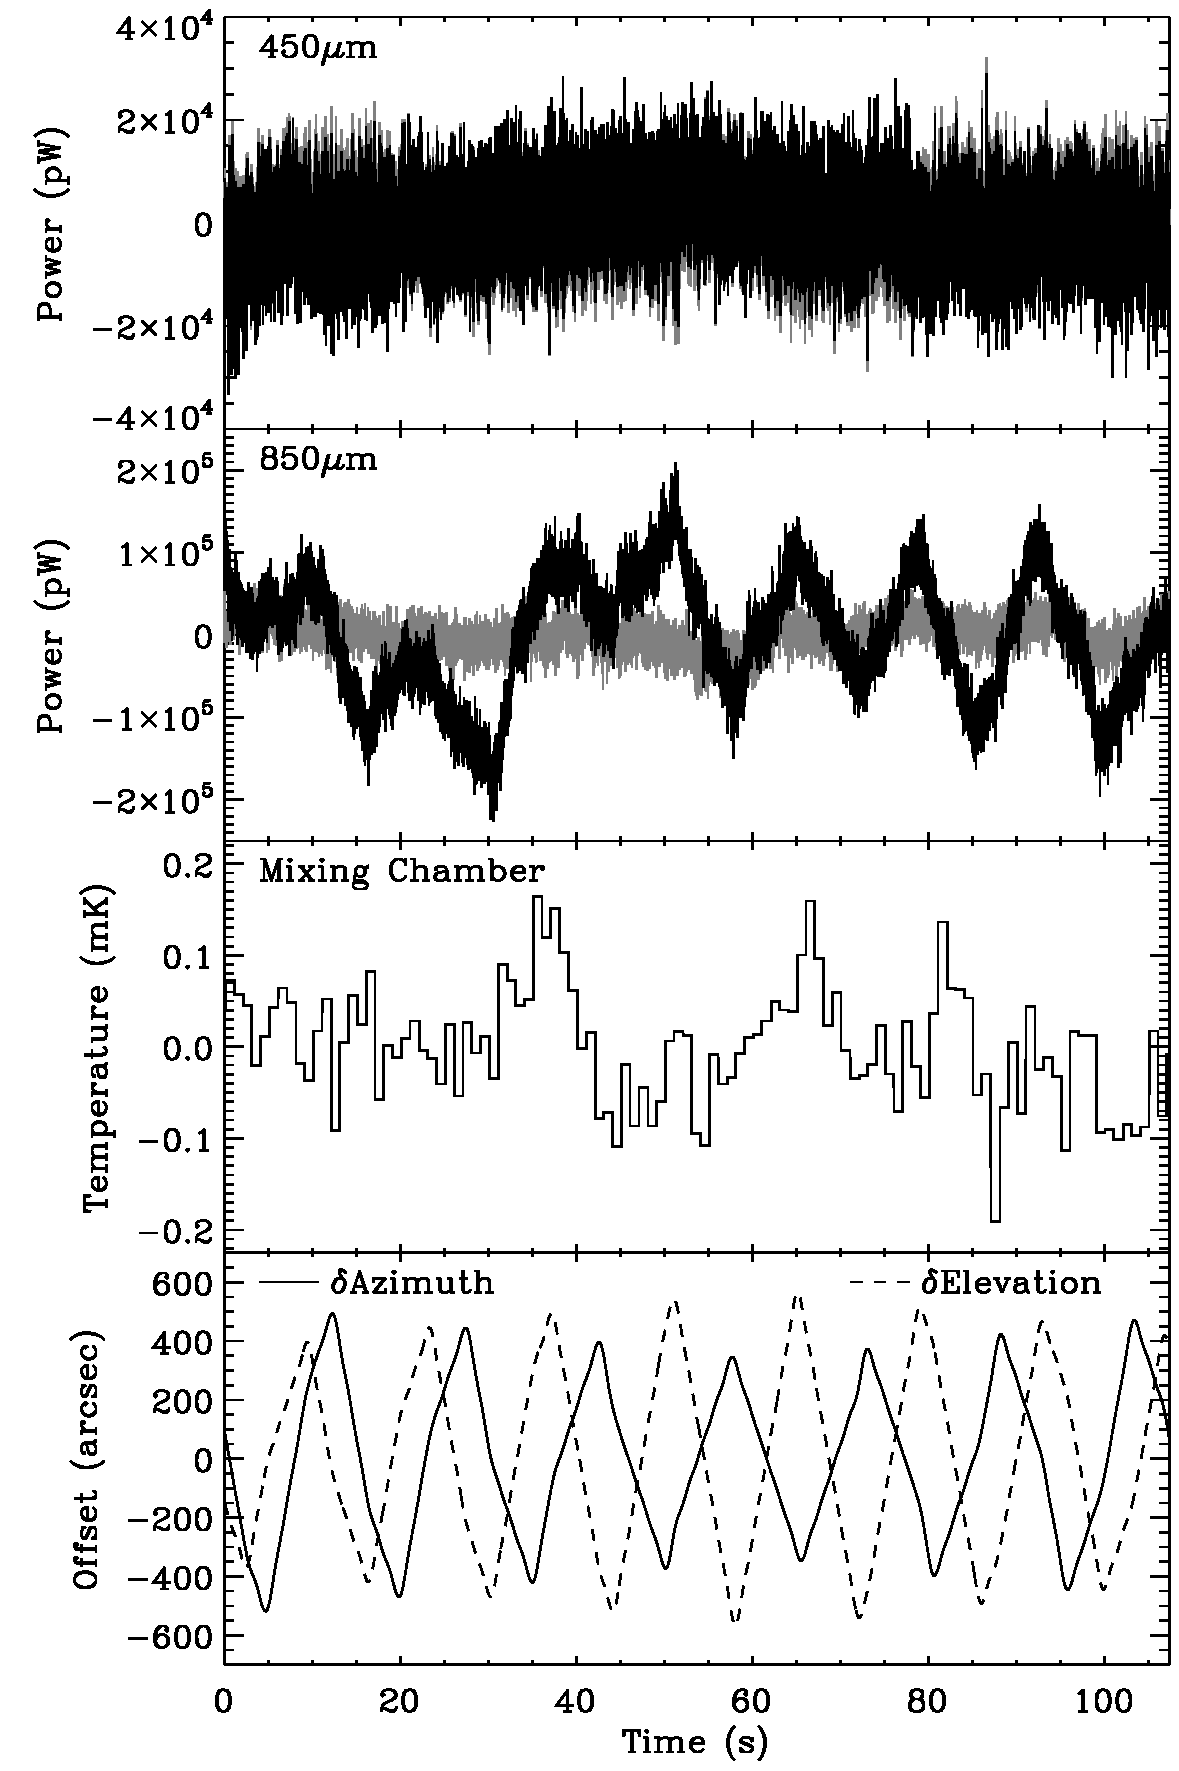
\includegraphics[width=\linewidth]{bolos_point_mix.pdf}
\caption{A comparison between single bolometer time series in each
  band (top two plots), with the mixing chamber temperature and
  azimuth/elevation pointing offsets. There is a strong correlation
  between the bolometers and the roughly $\sim$25\,s oscillation in
  the fridge, but not with the telescope motion. Also note that the
  total power in this primary signal is similar at both 450 and
  850\,\micron, pointing to an internal rather than an external
  source. The grey signals overplotted in the top-two panels show the
  residual time-series after removing the common-mode signal. This
  operation shows: (i) that most of the low-frequency signal is common
  to all of the bolometers; and (ii) the non-correlated, and
  predominantly white noise at 450\,\micron\ is significantly larger
  than at 850\,\micron.}
\label{fig:bolos_mix}
\end{figure}

Both bolometers share significant long-timescale structure
($\gsim10$\,s) that appears to be related to variations in the fridge
base temperature, although the similarity is clearly greater at
850\,\micron. In this particular case, the total power in the
fluctuations at 450\,\micron, from $-0.04$\,pW to $+0.08$, are larger
than the $-0.03$\,pW to $+0.05$\,pW fluctuations at 850\,\micron. Such
behaviour might be expected if there is a comparable varying thermal
load from the fridge at each wavelength, but a larger contribution of
atmospheric variations through the 450\,\micron\ bandpass filters. We
also note that there is no obvious strong correlation between the
low-frequency signal structure, at either wavelength, with the
telescope motion.

The low-frequency signal component of the bolometer signals is also
highly correlated amongst bolometers in the same subarray. We have
calculated a common-mode signal, $\mathbf{c}(t)$, as the average time
series of all the working bolometers. We then fit the amplitude of
$\mathbf{c}(t)$ at each wavelength to the signals shown in
Fig.~\ref{fig:bolos_mix} and remove it, yielding the grey residual
signals. These residuals are quite flat, although still with
noticeable variations. The white noise is also apparent, and larger at
450\,\micron\ as one would expect from the larger backgrounds compared
to 850\,\micron.

Next, we produce power spectral density (PSD) plots for several
representative bolometers in Fig.~\ref{fig:pspec}. To produce this
figure, we follow the convention that the PSD as a function of
frequency, $\mathbf{P}(f)$, is normalized such that the integral over
frequency gives the same variance as the time-series variance across
the full time series. In other words, given a bolometer signal
$\mathbf{b}(t)$,
%
\begin{equation}
\label{eq:psd}
\langle\mathbf{b}^2(t)\rangle = \int \mathbf{P}(f) df .
\end{equation}
%
However, we only show the PSD up to the Nyquist frequency, so the
conversion from variance measured in the frequency domain to the time
domain requires and additional multiplcation by 2; hence the units are
pW$^2$\,Hz$^{-1}$ rather than pW$^2$\,s.

\begin{figure}
\centering
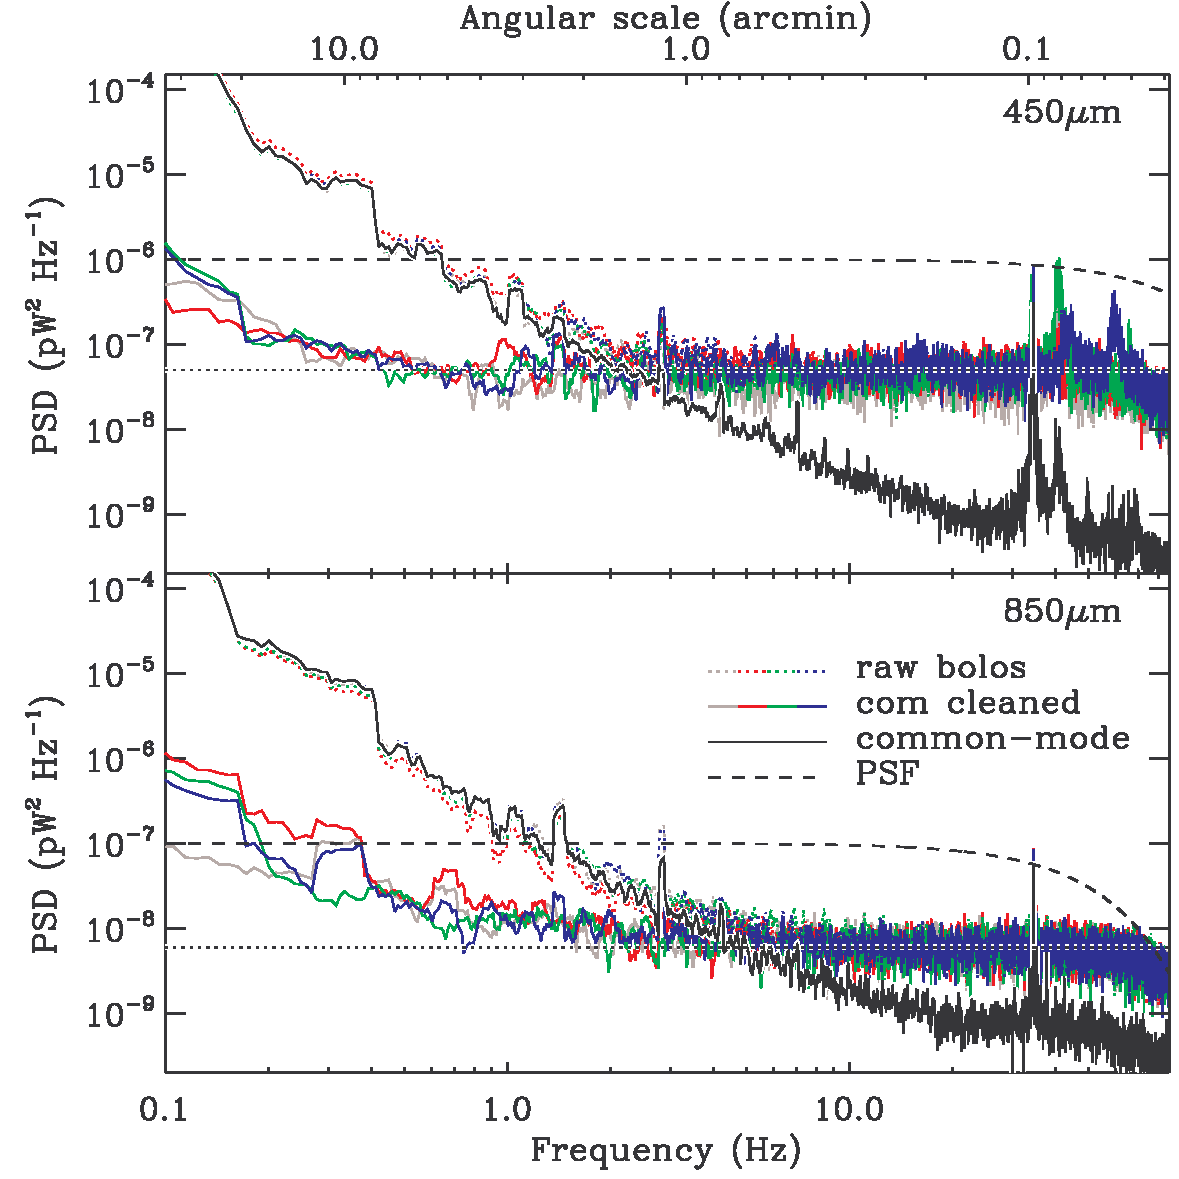
\includegraphics[width=\linewidth]{pspec.pdf}
\caption{Bolometer power spectral densities. Four representative
  bolometers have been selected from each sub-array, and the
  flat-fielded (but otherwise raw) PSDs are shown as coloured dotted
  lines (the blue signals are for the same time series as those shown
  in Fig.~\ref{fig:bolos_mix}). Horizontal dotted lines at $5 \times
  10^{-8}$ and $5 \times 10^{-9}$\,pW\,Hz$^{-1}$ at 450 and
  850\,\micron\ respectively, give the approximate white-noise
  levels. There are broad line features in the PSDs at both
  wavelengths above $\sim$35\,Hz. From $\sim$50\,Hz up to the Nyquist
  frequency, the gradual roll-off of the anti-aliasing filter is also
  evident.  At lower frequencies, the bolometer signals exhibit clear
  $1/f$ knees at approximately 2 and 4\,Hz at 450 and
  850\,\micron. The solid black lines are the PSDs of the common-mode
  signals at each wavelength, and the solid coloured lines show the
  PSDs of the bolometers once the common-mode is removed. These
  residual signals have significantly lower $1/f$ knees, approximately
  0.4 and 2\,Hz at 450 and 850\,\micron. Finally, the dashed black
  lines show the spectral shape produced by a point source, assuming
  that the telescope is slewing at 200\,arcsec\,sec$^{-1}$ (typical
  for S2SRO); for reference, the top horizontal axis shows the
  conversion from frequency to angular scale. We can see that the line
  features may add significant noise on the scale of the PSF. We also
  see that, for this scan velocity, the low-frequency noise begins to
  dominate on scales of approximately 8.3 and 1.7\,arcmin; these scales
  are comparable to the array footprint.}
\label{fig:pspec}
\end{figure}

The dotted coloured lines in Fig~\ref{fig:pspec} show the PSDs for
raw, though flatfielded data. At each wavelength, there is a clear
$1/f$ knee at a few Hz, followed by a predominantly white spectrum
punctuated by line features above $\gsim 30$\,Hz, and finally roll-off
caused by the anti-aliasing filter above $\gsim 70$\,Hz. As indicated
in the previous section, the correlation between the low-frequency
components of the different bolometer signals is large. The solid
black lines in Fig.~\ref{fig:pspec} indicate the PSDs of the
common-modes $\mathbf{c}(t)$ at each wavelength, which reproduce most
of the low-frequency structures, as well as the high-frequency line
features. The $\mathbf{c}(t)$ otherwise drop substantially below the
individual bolometer PSDs at high-frequency as expected if the
bolometers are dominated by un-correlated white noise. Finally, we
note that the amplitudes and slopes of the $\mathbf{c}(t)$ are similar
at both 450 and 850\,\micron. However, since the 450\,\micron\ white
noise is larger than at 850\,\micron\ (shown approximately by the
horizontal dotted lines), the $1/f$ knee occurs at a \emph{lower}
frequency at 450\,\micron.

Next, the common-mode signals are fit to each bolometer time series
and removed as in Fig.~\ref{fig:bolos_mix}, and the resulting PSDs are
shown as solid coloured lines. In this example, the residual signals
have $1/f$ knees significantly lower than in the raw PSDs.

For reference, the top horizontal axis has been converted to angular
scale assuming a scan velocity of 200\,arcsec\,sec$^{-1}$ which was
typical of the S2SRO observations. The power spectra of the PSFs in
each band (arbitrary normalized to peak values of $10^{-6}$ and
$10^{-7}$\,pW$^2$\,Hz$^{-1}$ at 450 and 850\,\micron\ respectively)
are also showed as dashed lines for this assumed scan velocity showing
that the smallest features resolvable by the telescope may be slightly
affected by the excess noise in the line features. At the lower
frequency end, the $1/f$ noise dominates at scales $\gsim 2$\,arcmin
in the raw data and $\gsim 10$\,arcmin in the common-mode cleaned data
at 450\,\micron, and at scales $\gsim 1$\,arscmin in the raw data and
$\gsim 2$\,arcmin in the common-mode cleaned data at 850\,\micron.

\subsection{Magnetic field pickup}
\label{sec:magpickup}

An additional noise source that appears to be significant in only a
small subset of the S2SRO data is magnetic field pickup. Since the
bolometer signals are ultimately detected through the amplification of
magnetic fields, any additional changing fields within the cryostat
will also be detected.

An example of an observation where pickup appears to be significant is
shown in Fig.~\ref{fig:magpickup}. The time-series for two
450\,\micron\ bolometers in the same column (not flatfielded) show
that there is a strong signal with a similar shape, but opposite
signs. This behaviour is seen across the entire array. The dark squid
signal for the same columns exhibits a similar shape and
amplitude. Since the dark squid has no thermal absorber or TES
attached to it, this observed signal is not likely to be optical or
thermal in nature (although there can be some crosstalk with the
bolometers...). It is also for this reason that the higher-frequency
noise that appears in the bolometer data (thermal) does not appear in
the dark squid, leading to a significantly higher \snr. The sign of
such a signal is expected to be random in the bolometer time-series
(ask detector person for an explanation).

\begin{figure}
\centering
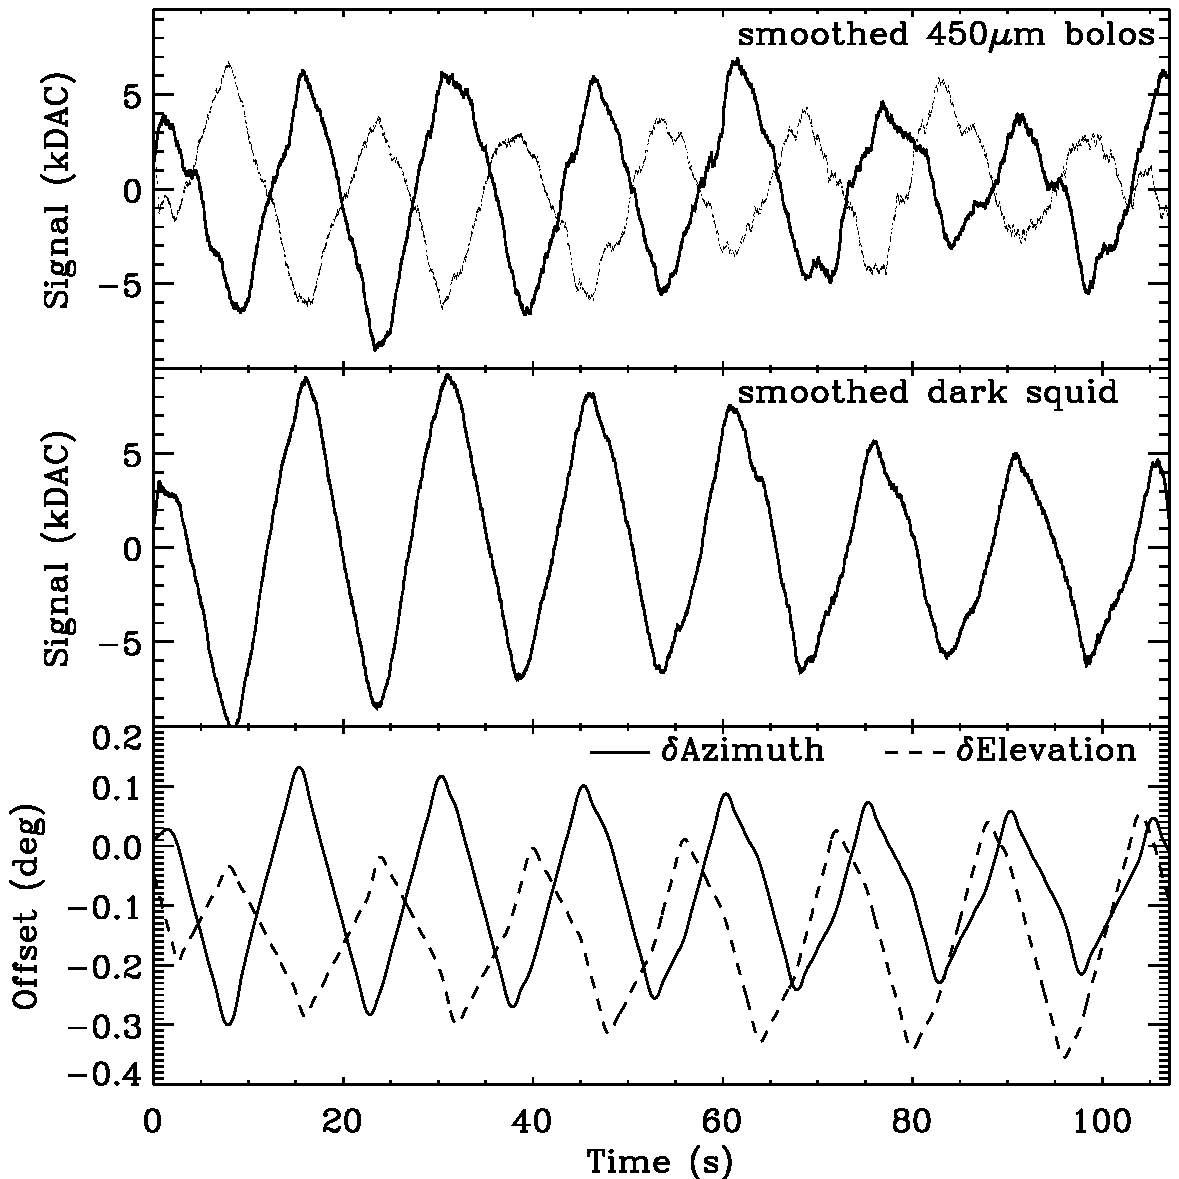
\includegraphics[width=\linewidth]{magpickup.pdf}
\caption{Evidence for significant magnetic field pickup for
  observation 20100228\_00016.  The top panel shows two un-flatfielded
  (but mean-subtracted) bolometer time-series from the same column,
  with a 200 sample boxcar smooth (approximately 1\,s), illustrating
  that they are dominated by a similar signal with opposite signs. The
  second panel shows the dark squid signal for the column, also
  mean-subtracted and with the same boxcar smooth. The bottom panel
  shows the azimuthal and elevation offsets from the map centre. For
  reference, the mean azimuth was 171.9\,deg, and the mean elevation
  68.0\,deg. Only the azimuthal signal appears to be correlated with
  the dark squids and bolometer signals, which suggests a magnetic
  field stationary with respect to the telescope dome as the source,
  since its direction with respect to the cryostat only changes with
  azimuthal motion.}
\label{fig:magpickup}
\end{figure}

The telescope pointing offsets for this approximately 0.5\,deg
diameter scan are also shown in Fig.~\ref{fig:magpickup}. Since the
phase of the azimuth offsets from the map centre in this scan pattern
slowly drifts with respect to the elevation offsets, it is clear that
the bolometer and dark squid signals are detecting a noise source that
is correlated only with the azimuthal motion and \emph{not} the
elevation. This behaviour would be expected if if there were a strong
magnetic field fixed with respect to the telescope dome (i.e., the
earth's magnetic field). Since \scuba\ is mounted on a Nasmyth
platform, only azimuthal motion will change the effective direction of
such a field with respect to the cryostat. It is also worth noting
that the absolute azimuth of the telescope was close to 180\,deg
(i.e., nearly due-south). We suspect that this observing
configuration, combined with the large amplitude of the scan, may have
conspired to produce these large signals.

%-------------------------------------------------
\subsection{Differences between the S2SRO and 2011 re-commissioned instrument}
\label{sec:s2sro}
%-------------------------------------------------

The S2SRO period took place during February and March 2010. For the
purpose of this paper, we will consider data taken as early as 2009
December 3, at which point the instrument was being commissioned in a
similar configuration to that of the S2SRO period. At this time, each
of the 450 and 850\,\micron\ focal planes were populated with single
subarrays, s4a and s8d respectively. There were two main mechanical
problems to contend with during this period. First, the fridge was not
able to cool the focal plane to the desired base temperature of
... which affected stability, particularly at 850\,\micron. Second,
there were problems with the subarray fabrication process which led to
large numbers of dead pixels, as well as large-scale variations in
$T_\mathrm{C}$ and the thermal conductivity, $G$. These latter issues
made it difficult to simulataneously place all of the TESs into the
optimal region of the superconducting transition, leading to
significantly poorer sensitivities.

While there were moderate variations from night-to-night during the
observing period, there were typically 600 to 900 working detectors in
each of the s4a and s8d subarrays. Fig.~\ref{fig:sensitivities} shows
representative responsivity maps for the two subarrays from the middle
of S2SRO based on the response to ramping the bolometer heaters.

%-------------------------------------------------
\subsection{Principal component analysis}
\label{sec:pca}
%-------------------------------------------------

A method that has been employed by teams analyzing BOLOCAM and AzTEC
data to identify and remove correlated noise is Principal Component
Analysis \citep[PCA,][]{laurent2005,scott2008}. We initially used PCA
to gain further insight into the nature of the \scuba\ noise
properties, but it is now also included it in SMURF as method for
cleaning the data.

The basic method is as follows: (i) a covariance matrix is built up
for all pairs $(i,j)$ of the $N$ bolometer time series,
$\langle\mathbf{b}_i(t),\mathbf{b}_j\rangle$; and (ii) a singular
value decomposition is used to identify a new set of statistically
uncorrelated eigenvectors, $\mathbf{\xi}_i(t)$ (i.e. whose covariance
matrix is diagonal), such that each of the bolometer time series is a
linear combination of the eigenvectors, or \emph{components}
i.e. $\mathbf{b}_i(t) = \bar{\mathbf{\xi}} \mathbf{\lambda}_i^T$,
where each row of the matrix $\bar{\mathbf{\xi}}$ is an eigenvector,
and $\mathbf{\lambda}_i^T$ is a column vector containing the
corresponding eigenvalues. The $\mathbf{\xi}_i$ are normalized by
their \rms, so that the amplitude of each component is stored in the
eigenvalues. In the earlier analyses mentioned, the low-frequency
noise is assumed to be encapsulated in those components with the
largest eigenvalues. Removing the projection of the time series along
those components has been used successfully to reduce $1/f$ noise
while retaining most of the signal in point-like sources. There is an
implicit assumption in this analysis that the noise properties are
stationary.

One unique feature of the \scuba\ data is that one can perform a PCA
analysis of both the 450 and 850\,\micron\ data simultaneously. The
first 6 most significant modes of our analysis are shown in
Fig.~\ref{fig:pca}, with the eigenvectors in the top panels, and maps
of the eigenvalues in each subarray in the bottom panels.

\begin{figure*}
\centering
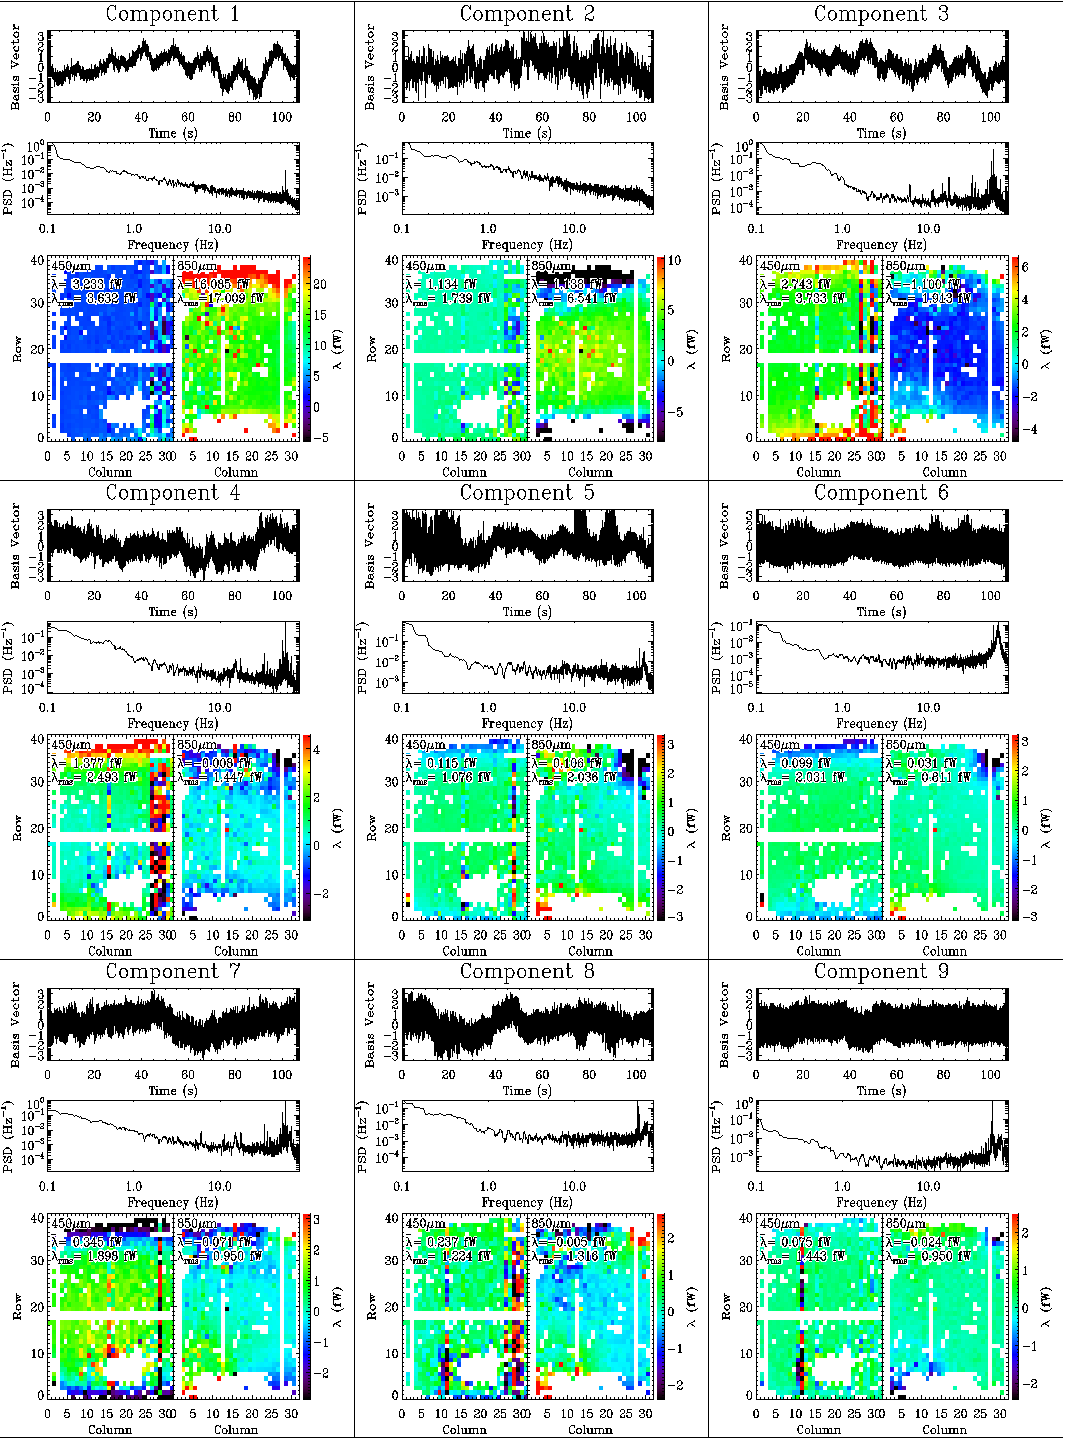
\includegraphics[width=\linewidth]{pca.pdf}
\caption{The first six modes from a principal component analysis,
  ordered by decreasing significance, of the combined 450 and
  850\,\micron\ time-series bolometer data. For each component, the
  top plot shows the time series of the eigenvector, normalized by its
  \rms. The bottom coloured panels show the eigenvalues for the
  bolometers at each wavelength (the amplitude of the eigenvector in
  the time series). For reference, both the mean, $\bar{\lambda}$, and
  \rms, $\lambda_\mathrm{rms}$, eigenvalues for the bolometers in each
  subarray are also shown. The first two components have comparable
  amplitudes, and dominate by at least a factor of 10 any other
  components of the time series. We suspect that they are caused by
  atmospheric variations (expected to be brighter at 450\,\micron),
  and fridge oscillations (expected to be comparable at each
  wavelength). However, the two eigenvectors do not necessarily map
  directly to these physical sources under this interpretation; rather
  they are two \emph{different} linear combinations of the underlying
  physical signals that give rise to statistically uncorrelated
  components. The third component accurately reproduces an apparent
  data-acquisition glitch that appears only at 450\,\micron\ (see
  Section ???). The fourth component is a ...\,Hz line feature only
  observed in column 15 of the 450\,\micron\ subarray. The fifth
  component shows a series of steps and glitches that appear
  predominantly along the bottom-left edge of the 850\,\micron\
  subarray where the bolometers are only tenuously locked. Finally,
  the sixth component is degenerating into a less significant, and
  more randomly scattered signal across the focal plane. Subsequent
  components follow this trend, and would generally be kept in a
  PCA-cleaning procedure.}
\label{fig:pca}
\end{figure*}

The majority of correlated signal at both wavelengths is clearly
broken down into the first two plotted components. The first dominates
at 450\,micron, whereas the second dominates at 850\,micron. For
reference, the eigenvalues of these two modes are in the range
$\sim1$--4\,pW, whereas the remaining modes have eigenvalues
$\lsim0.3$\,pW. As mentioned earlier, one simple model for the
correlated signal is a simple combination of oscillations in base
temperature (which would be similar in each band), with a varying
atmospheric signal (which is expected to be stronger at
450\,\micron). Indeed, the fainter component 2 most closely resembles
the mixing chamber temperature variations (Fig.~\ref{fig:bolos_mix}),
whereas component 1 is stronger at 450\,\micron\ and does not resemble
the fridge signal as closely.

This physical interpretation of the eigenvectors should, however, be
taken with a grain of salt, since the PCA analysis is really a
statistical black box. Suppose most of the low frequency noise really
could be decomposed into two components, the fridge signal
$\mathbf{F}(t)$, and an atmospheric signal $\mathbf{A}(t)$. The two
eigenvectors obtained from the PCA analysis are simply linear
combinations of $\mathbf{F}(t)$ and $\mathbf{A}(t)$ that are
statistically uncorrelated. Depending on the particular realizations
of these two noise sources, this decomposition may, or may not give
rise to eigenvectors that resemble the two underlying physical
sources. Regardless, similar analyses of a few data sets during S2SRO
give comparable results; most of the signal at both 450\,\micron\ and
850\,\micron\ appears to be produced by two dominant underlying
mechanisms.

The subsequent components identified by the PCA analysis in
Fig.~\ref{fig:pca} vary wildly. Component 3, though not obvious from
its eigenvector plot, is almost a pure ramping waveform that only
appears in the s4a data, and produces the broad line featuress
centered over 45\,Hz and 70\,Hz in the 450\,\micron\ PSDs in
Fig.~\ref{fig:pspec}. In other data sets, this third component has
also often instead exhibited a regularly-spaced series of spikes with
heights quantized into several amplitude families (again, only in the
s4a array). In both cases, the shape and phase of this signal is the
same in each bolometer, although the amplitude (and sign) varies, as
evidenced by the large random scatter in the s4a eigenvalue maps. It
is thought that these features are some sort of data acquisition
glitch as the spikes (when they appear) exhibit the expected point
response function of the anti-aliasing filter. Similarly, component 4
also appears to be a data acquisition glitch in the s4a array,
although along a single column, and with a peak at a lower frequency
of 40\,Hz, and a second feature right at the Nyquist frequency.

The last two components in Fig.~\ref{fig:pca} have an entirely
different character. The amplitudes of both components are greatest in
low-responsivity regions of the two subarrays (lower-right at
450\,\micron\ and bottom-left at 850\,\micron). Bolometers in these
regions of the subarray are probably only tenuously locked, and are
more sensitive to changes in the loading, possibly resulting in the
step and spikes that are seen in component 5. Component 6 is clearly
related to component 5, though with the absence of the steps and
spikes, so that together they seem to represent a continuum of shapes
that are linear combinations of the spikes and steps with the slower
drift evident only in component 6.

%------------------------------------------------------------------------------
\section{The SMURF Algorithm}
\label{sec:algorithm}
%------------------------------------------------------------------------------

Given \scuba's data rate, SMURF was designed with two primary goals in
mind: (i) reduced maps should be scientifically useful and of ``near
publication quality'' with minimal user interaction; and (ii) the
execution time should not appreciably exceed the amount of time
required to conduct observations on a high-end multi-tcore desktop
computer. By attaining these goals it would be possible to conduct
real-time reductions at the telescope to offer feedback to observers,
and it would also be possible to maintain a central repository of
(nearly) publishable data products.

As described in the introduction, rather than pursue a slow but
potentially more accurate \emph{maximum likelihood} method that would
require the inversion of a complex linear problem, we instead use an
iterative approach that estimates and removes most of the correlated
(and in particular low-frequency) noise sources in parallel with a
simplified map estimation. We do note, however, that recent advances
in direct inversion methods such as \citet{patanchon2008} may in fact
be tenable for \scuba\ data. A future goal of the software team is to
investigate meshing SMURF (perhaps as a cleaning step and initial
condition) for a SANEPIC-like algorithm.

The remainder of this section gives an overview of the model that is
assumed by SMURF for the \scuba\ data, and the typical steps used to
estimate a map. Subsequent sections discuss problems with this model
and additional processing steps and constraints that can be used to
improve the solution in different cases.

\begin{itemize}

\item Describe the bolometer signal model, and with the help of a flow-chart
show the basic procedure that SMURF follows.

\item Discuss SMURF configurability

\item Some sort of proof/demonstration showing why the algorithm works

\item Discuss performance (execution time, memory, disk usage etc.)

\item Where do you get SMURF/starlink, usage of NDF

\item Talk about pipeline?

\end{itemize}

We express the signal observed by the $i$th bolometer as a function of time,
\begin{equation}
\mathbf{b}_i(t) = g_i[\mathbf{e}_i(t) \mathbf{a}_i(t) + \mathbf{n}_i(t)]
\end{equation}
where $\mathbf{a}(t)$ is the time-varying signal produced by scanning
the telescope across astronomical sources, $\mathbf{e}(t)$ is the
time-varying extinction, which is a function of the telescope
elevation and atmospheric conditions, and $\mathbf{n}_i(t)$ represents
sources of noise. The two terms in square brackets, as written, have
units of power delivered to the detectors (pW). The scale factor $g_i$
converts this effective power to the digitized units recorded on disk
(DAC) -- the \emph{flatfield} multiplied by a digitization constant --
and in this formulation it is assumed to be constant in time.

We then express the noise, $\mathbf{n}_i(t)$, as the sum of several
components,
%
\begin{equation}
  \mathbf{n}_i(t) = \mathbf{n}^\mathrm{w}_i(t) + \mathbf{n}^\mathrm{f}_i(t) +
  \mathbf{n}^\mathrm{c}(t),
\label{eq:noise}
\end{equation}
%
where $\mathbf{n}^\mathrm{w}_i(t)$ is uncorrelated white (thermal)
noise, $\mathbf{n}^\mathrm{f}_i(t)$ is low-frequency noise that is
\emph{not} correlated from bolometer-to-bolometer, and
$\mathbf{n}^\mathrm{c}(t)$ is a (predominantly low-frequency)
correlated or \emph{common-mode} component. The primary goal of
map-making is to model and remove $\mathbf{n}^\mathrm{f}_i$ and
$\mathbf{n}^\mathrm{c}$ from the time-series, while re-gridding the
remaining data we can then hope to approach the theoretical noise
limit in the map. This procedure is summarized in Fig.~\ref{fig:dimm}.

\begin{figure}
\centering
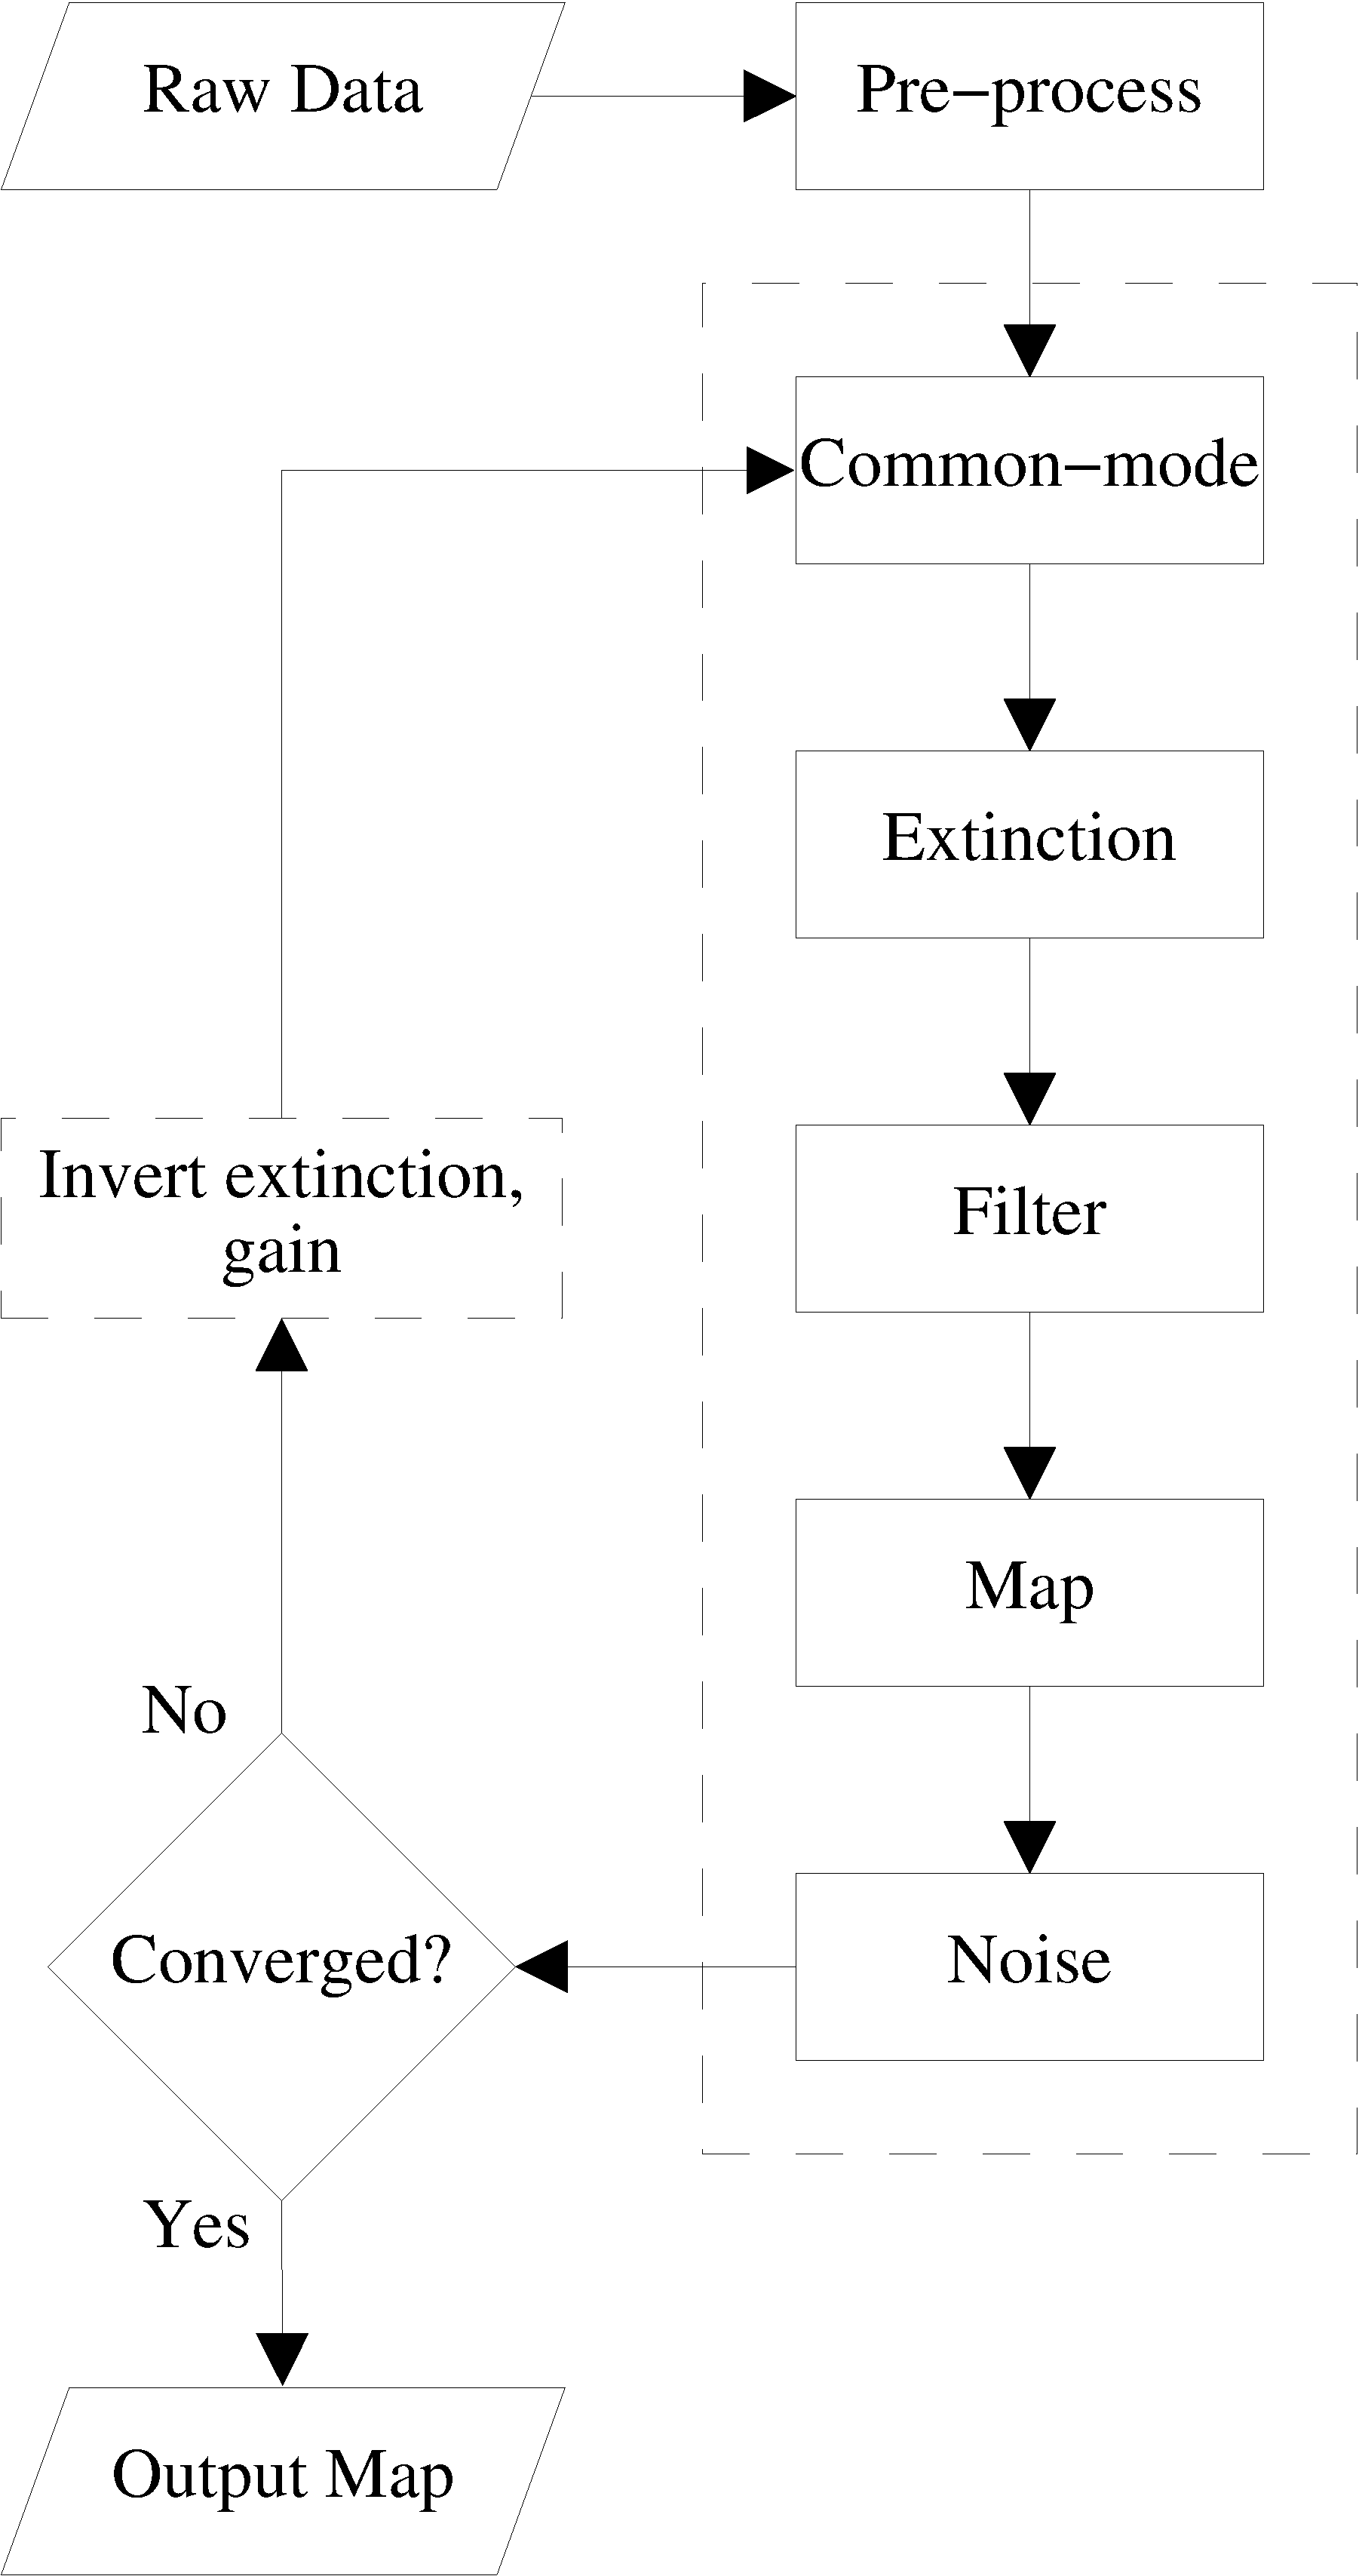
\includegraphics[width=0.75\linewidth]{dimm.pdf}
\caption{Typical map-making algorithm. Raw data (stored in multiple
  files) are read and concatenated into continuous time series. A
  pre-processing stage repairs DC steps, applies a flatfield
  correction, and identifies and removes the noisiest bolometers. The
  iterative portion then begins: estimating and removing the
  common-mode signal; applying the extinction correction; high-pass
  filtering to remove residual independent low-frequency noise;
  estimating the map by re-gridding the data; and finally measuring
  the noise in the residual time series. If the \rms\ has converged,
  the final map is written to disk. Otherwise any multiplicative
  factors that may have been applied to the data are inverted (e.g.,
  extinction correction and relative gains measured during the
  common-mode calculation), and each additive component is added back
  into the time series and re-estimated in turn.}
\label{fig:dimm}
\end{figure}

First, the data files are read from disk, concatenated into contiguous
arrays in memory, and run through a pre-processing stage that performs
several operations including spike and sudden level step removal to
enforce continuity in the time-series. Then, the iterative process
within the dashed box begins. It is generally assumed that the
dominant noise component is the common-mode, which is presumably
dominated by large variations in the fridge temperature and sky noise
(as argued in Section~\ref{sec:pca}). This signal is estimated as the
average signal observed by all of the bolometers at each time step,
and then removed from all of the bolometers. Once this large signal
has been removed, we apply the extinction correction, which is
determined completely from external measurements
\citep[see][]{dempsey2012}. Next, residual noise that differs from
bolometer-to-bolometer (primarily low-frequency) is removed, usually
using a high-pass filter. The resulting ``clean'' time-series are then
re-gridded to produce a map estimate using nearest-neighbour
sampling. Since each map pixel is calculated as the average of many
bolometer samples, it is fundamentally much less noisy than the raw
bolometer time-series. We can therefore project the map back into the
time domain (i.e. scanning the array across the current estimate of
the map), and create approximately noiseless estimates of what each
bolometer would have seen in the absence of noise sources, and remove
that from the time-series. This final step in the iteration gives a
residual signal (with low-frequency and astronomical noise components
removed) that may be used to measured the white noise level in each
detector, and also to estimate an approximate $\chi^2$ for the model
to track convergence. As we will discuss in the next sections, each
signal component estimate is biased slightly from the presence of
signal from other components, so the entire process is
iterated. However, before the next iteration begins, we first undo the
multiplicative factors introduced by the extinction correction, and
also relative gains that may optionally be estimated in the
common-mode estimation phase.

In practice, the map-maker is highly configurable, both in terms of
the order in which model components are fit (and whether they are fit
at all), and the details of \emph{how} they are fit. A summary of the
model components is given in the next section.

%-------------------------------------------------
\subsection{Model components}
\label{sec:components}
%-------------------------------------------------

In addition to specifying when each model component is calculated
(normally an attempt is made to order them by decreasing amplitude in
the time-series), there are a number of parameters that control their
operation. Table~\ref{tab:components} lists the model components and
the typical order in which they are calculated. The following sections
describe their implementation in detail.

\begin{table}
  \caption{Summary of the model components that can be fit to
    \scuba\ time-series data with SMURF. Only the first group of
    models (in the order indicated) are typically fit to the data
    (\model{COM}--\model{NOI}) in the indicated order. The remaining
    models (\model{DKS}--\model{PLN}) have only been included for
    completeness}
  \vspace{0.2cm}
  \centering
  \begin{tabular}{c|l}
    \hline
    Model & Description \\
    \hline
    \model{COM} & remove common-mode signal \\
    \model{GAI} & common-mode scaled to each bolometer \\
    \model{EXT} & extinction correction \\
    \model{FLT} & Fourier transform filter \\
    \model{AST} & map estimate of astronomical signal \\
    \model{NOI} & noise estimation \\
    \hline
    \model{DKS} & dark squid cleaning along columns \\
    \model{PLN} & 2-dimensional time-varying plane removal \\
    \model{SMO} & time-domain smoothing filter \\
    \model{TMP} & pointing as baseline template \\
    \hline
    \end{tabular}
  \label{tab:components}
\end{table}

\subsubsection{\model{COM,GAI}: common-mode estimation}
\label{sec:comgai}

Fig.~\ref{fig:com} shows the time series from a selection of typical
bolometers.\footnote{The data have been flat-fielded and each time series
has been adjusted to a mean value of zero.} The similarity between most
bolometers is evident, and forms the common-mode signal - assumed to be a
consequence of variations in the atmospheric emission and fridge
temperature. This common-mode usually dominates the astronomical signal
for all but the brightest sources, and swamps faint extended structure.
The purpose of the \model{COM} and \model{GAI} models is to remove this common-mode
signal.

\begin{figure}
\centering
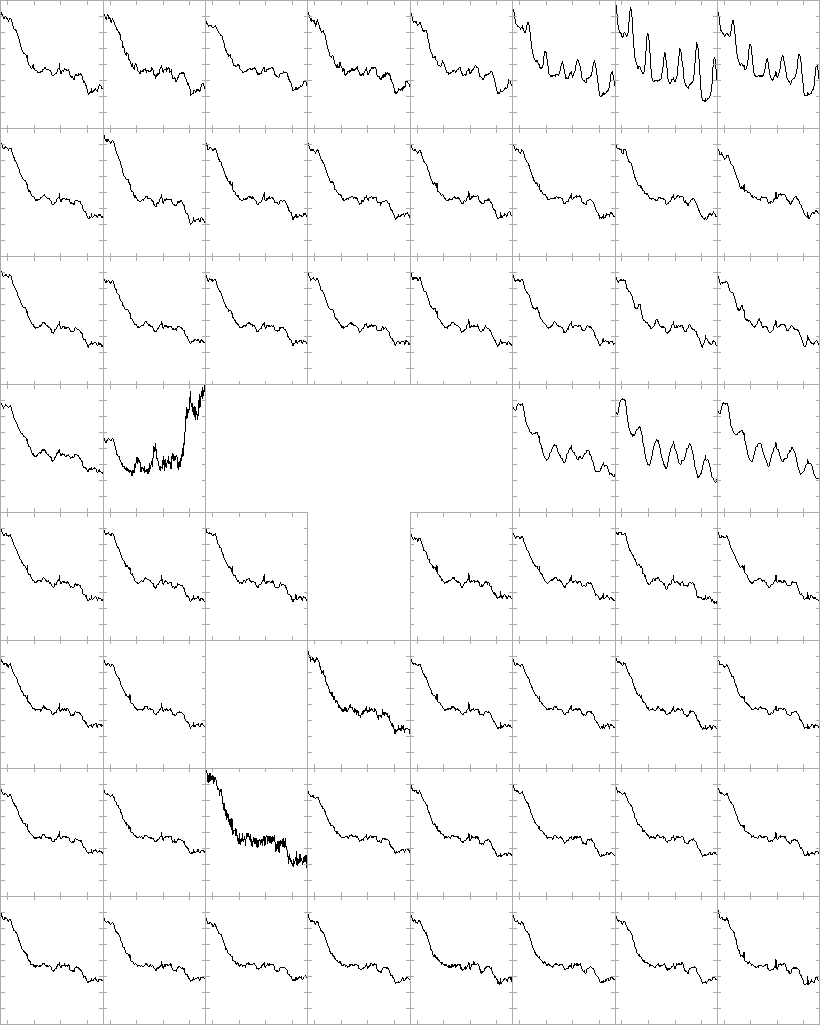
\includegraphics[width=\linewidth]{com.pdf}
\caption{A selection of typical bolometer time series after flatfielding
and removal of a constant baseline. It can be seen that most bolometers
exhibit a common time variation overlayed with other features.}
\label{fig:com}
\end{figure}

The \model{COM} model is the common-mode signal itself. It is a single time
series that is estimated by finding the mean of all bolometers at each
time step. Bolometer values that have been flagged as unusable for any
reason are excluded from the mean.

Since bolometers have varying sensitivities, the amplitude of the
common-mode variations will also vary from bolometer to bolometer. So
comparing each bolometer time stream with the common-mode signal
allows an estimate of the bolometer sensitivity to be obtained. In
practice, a least squares linear fit is performed between the
bolometer time series and the common-mode to determine a gain and
offset for each bolometer.  The gain and offset for each bolometer is
known as the \model{GAI} model. Each bolometer value can then
optionally be scaled and shifted using these values so that all
bolometers share a common (but as yet unknown) calibration. This
provides an alternative( or additional) flatfielding strategy to that
described in in section~\ref{sec:bolos}.

An option exists to cater for time-varying sensitivities. If used, the
least squares fits described above are performed on short blocks of
contiguous time slices, providing multiple gain and offset values for
each bolometer (one pair for each block of time slices). The gain and
offset at any required time slice can then be found by interpolation
between these values.

It can be seen from Fig.~\ref{fig:com} that some bolometers depart
radically from the common-mode, indicating some problem within the
bolometer. Such bolometers are identified by calculating the Pearson
coefficient of correlation between each bolometer time stream and the
common mode. Bolometers for which the correlation coefficient is below a
specified limit, or which have a negative gain, are flagged as bad in
order to omit them from the final map. If the option described above for
handling time-varying sensitivities is used, then a correlation
coefficient can be determined for each individual block of time slices.
This allows individual bad blocks to be rejected from a bolometer time
stream, rather than rejecting the whole bolometer. This is beneficial for
bolometers that follow the common-mode for most of the time but suffer
from transient problems at specific times.

The common-mode is calculated from all bolometers that have not
previously been flagged as bad. Thus aberrant bolometers with low
correlation coefficients will be included, polluting the common-mode. For
this reason, an iterative approach is taken to estimating the common-mode.
The initial common-mode estimate is formed from all remaining bolometers.
Aberrant bolometers with low correlation coefficients are then identified
by comparing each bolometer time stream with the common-mode. Such
aberrant bolometers are flagged as bad, and a new estimate of the
common-mode is produced omitting the newly flagged bolometers. This
process is repeated until no further bolometers are rejected.

Any astronomical sources that are smaller than the array size will
contribute signal to some bolometers but not other bolometers, thus
biassing the simple mean used to estimate the common mode. However, on
each iteration of the map-making algorithm illustrated in
Fig.~\ref{fig:dimm}, a large fraction of the remaining astronomical
signal is extracted from the bolometer time series and transferred to the
output map, resulting in subsequent estimates of the common-mode being
more accurate.

Any extended astronomical emission on a scale comparable to or larger
than the spatial extent of the area used to estimate the common-mode will
contribute a similar signal to all bolometers. Therefore such extended
emission is indistinguishable from the other sources of common-mode
signal (fridge and atmosphere variations) and will be removed by the
model. This places a limit on the spatial extent of astronomical
structure that can be recovered.

For this reason, the usual practice is to estimate a single
\model{COM} model by examining data from all four sub-arrays in each
waveband, since this allow spatial structure on the scale of the whole
focal plane to be recovered. However, sometimes there is evidence that
the common-mode differs from one array to another, and so an option
exists to estimate a separate \model{COM} model for each individual
subarray, with a consequent lowering in the scale of spatial structure
that can be recovered.

\subsubsection{\model{EXT}: extinction correction}
\label{sec:ext}

The extinction correction is a multiplicative factor that is normally
derived using the JCMT water vapour radiometer (WVM), and is not
considered to be a free parameter in the solution. However, it is
applied as part of the iterative solution, rather than a
pre-processing step, since any small errors will be amplified by the
large low-frequency drifts in the raw bolometer time-series. For
example, if the bolometer drift is 1000 times greater than an
astronomical source of interest, a 1 per cent error in the flatfield
will produce stripes of order 10 times the astronomical signal
amplitude in the final map! If \model{EXT} is applied after the bulk
of the low-frequency noise has been removed (e.g., \model{COM,GAI}),
then there is little potential for such small errors to affect the
final map.  For details on how it is calculated see
\citet{dempsey2012}. Note that its numerical value is calculated only
once, and simply applied as a scale factor in the iterative solution.

\subsubsection{\model{FLT}: fourier transform filter}
\label{sec:flt}

This model takes the FFT of the bolometer data, and can apply both
high- and low-pass filters, as well as notch filteres, at hard
frequency edges specified by the user. Alternatively, the frequency
edges of the filters may be defined in terms of an \emph{angular
  scale}, but converted into a frequency through knowledge of the mean
telescope slew speed. The time-series may optionally have apodization
applied before the transform to avoid ringing (primarily caused by
wrap-around discontinuities at the ends of the time-series). Finally,
a whitening filter may also be applied in which a simple $1/f^\alpha +
\mathrm{constant}$ is fit to the power spectrum of each bolometer, and
then the bolometer FFT is multiplied by its inverse (though normalized
to preserve the white noise level).  The signal that is \emph{removed}
from the time-series by this process are stored in the \model{FLT}
container array. Typically this model is used purely as a high-pass
filter to remove most of the $1/f$ noise. Low-pass filtering is
redundant for two reasons: (i) SMURF already low-pass filters and
re-samples to a lower sample rate as described in
Section~\ref{sec:downsamp}; and (ii) the act of re-gridding the data
to produce map estimates effectively low-pass filters the data at a
frequency that corresponds to the inverse of the crossing time of a
single map pixel. Notch filters have not been used with \scuba\ data
particularly since line features tend to move around (i.e. a dynamic
line-detection system would have to be developed, and care would have
to be taken that astronomical sources are not suppressed).

\subsubsection{\model{AST}: map estimation}
\label{sec:ast}

Map estimation is accomplished using a nearest-neighbour resampling of
the data onto a pre-defined map grid. For the $i$th map pixel
$\mathbf{m}(x_i,y_i)$, the brightness is estimated as the weighted
average of the bolometer data samples $\mathbf{b}_j$ that land within
that pixel (from any bolometer or point in time),
%
\begin{equation}
  \mathbf{m}(x_i,y_i) = \frac{\sum_j \mathbf{w}_j \mathbf{b}_j }
                             { \sum_j \mathbf{w}_j } .
\end{equation}
%
For the initial iteration the weights $\mathbf{w}_j$ are set to 1, but
subsequently they are set to $1/\sigma_j^2$, the estimated inverse
variance expected from the bolometer white noise levels as discussed
in Section~\ref{sec:noi}. This weighting scheme is sensible provided
that the bolometer data have no correlated (i.e., low-frequency)
noise.

In addition, a variance map $\mathbf{v}(x_j,y_j)$ is estimated. The
default behaviour is to estimate this weighted error on the mean given
the scatter in the weighted samples. This is accomplished by dividing
the \emph{biased weighted sample variance} by the number of samples
that went into the average (akin to the formula for standard error on
the mean, but accounting for weights),
%
\begin{equation}
\label{eq:varmap}
\mathbf{v}(x_j,y_j) = \frac{\sum_j \mathbf{w}_j
                            \sum_j \mathbf{w}_j \mathbf{b}_j -
                            \left( \sum_j \mathbf{w}_j \mathbf{b}_j \right)^2 }
                           { N \left( \sum_j \mathbf{w}_j \right)^2 },
\end{equation}
%
where $N_j$ is the total number of bolometer samples that land in the
pixel. As written, this algorithm is numerically unstable if the two
terms in the numerator are large, and of nearly the same value:
floating point precision errors can cause the difference to be
significantly incorrect. In practice we use the more numerically
stable ``weighted incremental algorithm'' that calculates incremental
differences, as described in \citet{west1979}.

 We decided not to use the \emph{unbiased} estimator since in
practice it would require accumulating an additional array of values
at every map pixel, and only results in a small difference where there
are less than $\sim10$ samples per pixel (a situation that is almost
never encountered in a \scuba\ map except in the edge pixels).

Finally, once the map estimation is complete, the map is projected
into the time domain (the signal that would be produced in each
bolometer by the signal represented by the map) and removed.

In addition to map estimation, the \model{AST} model can also be used
to perform map-based despiking of the time-series
(Section~\ref{sec:mapdespike}), and to apply constraints to the map to
improve convergences (Section~\ref{sec:converge}).

\subsubsection{\model{NOI}: noise estimation}
\label{sec:noi}

The primary purpose of the noise component, \model{NOI}, is to measure
the white noise of each bolometer ($\mathbf{n}^\mathrm{w}_i(t)$ in
Eq.~\ref{eq:noise}). The measurement generally occurs once all of the
other models have been fit and removed. This noise may then be used to
estimate weights for the data in subsequent iterations.

First, the bolometer PSDs are calculated as in Eq.~\ref{eq:psd}. An
average white noise level is then measured from 2 to 10\,Hz, a
relatively clean region of the PSD that tends to lie above the $1/f$
knee, but below the high-frequency line features for typical bolometer
data (Fig.~\ref{fig:pspec}). Taking this constant level for
$\mathbf{P}(f)$ we then calculate the expected variance of the
time-series (in approximately 200\,Hz samples) using
Eq.~\ref{eq:psd}. If the bolometer noise were produced purely by
uncorrelated thermal sources (i.e. no other long-scale drifts), with
no high-frequency line features, and without the attenuation at even
higher frequencies by the anti-aliasing filter, this is the
theoretical noise limit of the detectors. These measured variances are
stored, and then used in subsequent iterations to weight the data
points when calculating the map estimate (Section~\ref{sec:ast}). They
are also used for convergence tests (Section~\ref{sec:converge}).

Since noise estimation is usually calculated as the final step in the
iteration, it is the cleanest data for which some cleaning operations
may be performed. For this reason \model{NOI} can optionally use the
time-domain DC step fixer (Section~\ref{sec:steps}) and spike
detection (Section~\ref{sec:timedespike}).

Finally, it should be noted that the default behaviour is to calculate
the white noise levels \emph{once} within \emph{NOI}, after the second
iteration. The reason for fixing these values is to prevent any
potential divergence in the weight estimates with iterations, and also
to provide a fixed reference for the convergence tests
(Section~\ref{sec:converge}). Note that the absolute values of the
noise, and therefore weights calculated by the model component are
irrelevant (only their relative values). The reason is that the final
noise in the map is measured empirically from the scatter of the data
points that land in each pixel (Section~\ref{sec:ast}), and
large-scale noise sources can be checked by analyzing the angular
power spectra of jackknife maps (e.g., Section~\ref{sec:cosmo}).

\subsubsection{Other experimental models}

We don't use them, but we should mention them since a reviewer might
ask us if we tried them: \model{DKS}, \model{TMP}, \model{SMO},
\model{PLN}.


Columns share significant magnetic field pickup which is measured by
the dark squids. This model has been included although it makes little
improvement, or injects noise since the magnetic field pickup noise is
generally sub-dominant. Furthermore, not every column that contains
working bolometers also has a working dark squid. An alternative is to
use the \model{TMP} model described below.

\textit{There are also the popped bolometers that could help fill the
gaps.}

Since the \model{DKS} cannot generally be used due to the missing
dark squids, an alternative is to use the telescope pointing as a
proxy for the signal due to magnetic field pickup
(Section~\ref{sec:magpickup}. Generally speaking the azimuth (or its
sine) as a function of time is used as a template that is simply
scaled and removed from each bolometer signal. Some modest
improvements can be achieved with this model.

We also have the SMO filter that's useful for very short scans
because edge effects don't matter so much. Two sorts - median which is
more robust, or mean which is more accurate.

We can remove a plane at each timeslice but it doesn't seem to improve
things. Perhaps refer to other papers that claim to have seen coherent
2d structures in the sky noise?

\subsection{Convergence tests and model degeneracies}
\label{sec:converge}

The map-maker will halt if the convergence criteria have been
met. Presently there are two numerical tests that may be performed by
SMURF, or alternatively, a fixed number of iterations may be
specified. The first numerical test is an approximate check of the
change in reduced chi-squared, $\chi^2_\mathrm{r}$. The standard
deviations, $\sigma_i$, are measured for each of the residual
bolometer signals once the modeled signal components have been
removed. In the early iterations, the residual signals usually contain
both white noise, and other long-timescale features. However, once the
solution has converged, this signal should look approximately
white. Once the white nosie, $\mathbf{n}^\mathrm{w}_i(t)$, has been
measured from the bolometer PSDs in \model{NOI}
(Section~\ref{sec:noi}), $\chi^2_\mathrm{r}$ is calculated as $(1/N)
\sum_i \sigma^2_i / \mathbf{n}^\mathrm{w}_i(t)$, where $i$ runs over
the $N$ bolometers. In other words, it is the average ratio between
the measured time-series bolometer variances and their white-noise
levels measured between 2--10\,Hz. Note that this expression
\emph{does not account for the degrees of freedom}. Clearly there are
a large number of parameters in the model, which will ``fit-out'' some
of the uncorrelated white noise, and potentially bias this estimate of
$\chi^2_r$ low. One approach would be to keep track of the degrees of
freedom, and therefore provide a correction, as in
\citet{kovacs2008}. However, note that we are only using this value as
a convergence test, and its value is not used in an absolute
sense. Furthermore, the reference white noise values are calculated
only once in SMURF (Section~\ref{sec:noi}), and the number of model
parameters are fixed, so the value of $\chi^2_r$ should decrease
monotonically if the solution is behaving well. The convergence
criterion is met if the change in subsequent values of $\chi^2_r$ is
smaller than the parameter \texttt{chitol}, which is set to $10^{-3}$
by default.

It was immediately found in the analysis of \scuba\ data that the
$\chi^2_r$ test described above was not a sufficient stopping
criterion. The reason for this is that various components of the model
are, under normal circumstances, highly degenerate. One simple example
is the degeneracy between large-scale astronomical structures (larger
than the array footprint), and the common-mode rejection step
(\model{COM}), which will be illustrated in
Section~\ref{sec:point}. Since the flatness of the residual only
reflects the ability of the model to fit the shape of the bolometer
time-series, it does not necessarily correlate with convergence of the
most important model component: the map. Indeed, examination of the
map after large numbers of iterations (e.g., $>10$), shows the
presence of large-scale structures that are anti-correlated with
structures in other model components. For this reason, a second
map-based convergence test was added.

The map-based convergence statistic, $M_c$, is the average absolute
change in the value of map pixels between subsequent iterations,
normalized by the map pixel uncertainties (square root of
Eq.~\ref{eq:varmap}), or
%
\begin{equation}
M^j_c = \frac{1}{N} \sum_i \frac{| \mathbf{m}(x_j,y_j) -
  \mathbf{m}(x_{j-1},y_{j-1}) |} {\sqrt{\mathbf{v}(x_j,y_j)}} ,
\end{equation}
%
where $i$ runs over the $N$ map pixels, and $j$ enumerates
iteration. The convergence criterion is met once this average change
is smaller than the parameter \texttt{maptol}. Experimentally we found
that a threshold of 0.05 gives good results (on average, map pixels
change by 5\% of the estimated map RMS in subsequent iterations).
This provides good correspondance with what we would choose ``by
eye'', and furthermore, letting the solver run for many more
iterations in several test cases yields insignificant differences.

Another major source of divergence is correlation between \model{COM}
and \model{FLT}. Since \model{FLT} usually consists of a high-pass
filter following the application of \model{COM}, \model{COM} is
completely free to grow any large-scale structure at frequencies below
the chosen filter edge. While such structure does not appear in the
map (as it is removed by \model{FLT}), we found that the solution
could be made to converge significantly faster by ``re-mixing''
\model{COM} and \model{FLT} at the start of each iteration. In
practice, at the start of each iteration, the previous iterations of
each model are both added back into the residual immediately prior to
re-calculating \model{COM}. In this way, truly common-mode signals,
even at low-frequencies, do not leak into \model{FLT}.

%-------------------------------------------------
\subsection{Data cleaning}
%-------------------------------------------------

Since we can do most of this stuff either as a pre-processing step or
iteratively, I thinks this goes in a generic-sounding subsection. This
can go here, or perhaps earlier?

\subsubsection{Time-series down-sampling and map pixel size}
\label{sec:downsamp}

The highest useful frequency in the nominally 200\,Hz-sampled
\scuba\ data is that which corresponds to the smallest angular scale
that the instrument is sensitive to. As mentioned earlier, the usual
rule-of-thumb for a Gaussian beam is to provide at least 3 samples for
each FWHM, or roughly 2.5\,arcsec for the 7.5\,arcsec
450\,\micron\ channel, and 5\,arcsec for the 14.5\,arcsec
850\,\micron\ channel. For a typical scan speed of
300\,arcsec\,s$^{-1}$, the maximum useful sample rate is therefore
about 120\,Hz at 450\,\micron, and 40\,Hz at 850\,\micron. In order to
save execution time and memory usage (both of which scale linearly
with data volume), it is clearly advantageous to re-sample the data to
these lower rates.

Similarly, from the point of view of retaining all of the useful
information, the size of the output map pixels need not be any smaller
than the FWHM/3 rule. Larger pixels may be selected, but at the
expense of retaining information at the diffraction limit of the
telescope.

The default behaviour of SMURF is to select output map pixel sizes of
2 and 4\,arcsec at 450 and 850\,\micron, respectively (slightly
over-sampled). The slew speed of the telescope (approximately constant
for all standard scan modes) is then used to calculate the highest
useful frequency for the time-series given the map pixel size,
$f_\mathrm{max}$. The data are then re-sampled to this new rate prior
to map-making (as well as the data cleaning steps).

The method used by SMURF to down-sample simply averages together
multiple samples from the original time-series, $x_i$ to estimate the
lower-frequency output time-series, $y_j$. In general there will not
be an integer number of samples from $x_i$ in each of the $y_j$, so
fractional samples from $x_i$ are used at the $y_j$ time
boundaries. The algorithm is fast since each sample in $x_i$ need only
be visited once. From a spectral point of view, this boxcar average is
equivalent to applying a sinc-function low-pass filter in frequency
space. Such behaviour is desirable since it serves as an anti-aliasing
filter; most non-white features above the Nyquist frequency in $y_j$
that could contaminate the output data are largely removed.

As an alternative, we also investigated an algorithm in which the FFT
of $x_i$ is simply truncated to the target sample rate before
transforming back to the time domain (i.e., applying a hard-edged
low-pass filter). In practice the noise performance was
indistinguishable, and required slightly more execution time, using
this method compared to the boxcar method described above. It is
therefore not currently available to users.

\subsubsection{Bolometer Filtering}

Despite the ability of the map-maker to iterative remove many noise
components, under some circumstances it may be desirable to filter the
data \emph{once} during the pre-processing step. Three main filtering
options are available:

\begin{itemize}

\item The most commonly-used pre-processing filter is polynomial
subtraction. A polynomial of the requested order is fit and removed
from each bolometer time-series. At a bare minimum, the mean is
removed from all of the bolometers (order 0) in all reductions
described in this paper.

\item All of the filters available as part of the iterative Fourier
Transform Filter (Section~\ref{sec:flt}) can also be applied once
during pre-processing.

\item As a complete alternative to the iterative map-making procedure,
cleaning by principal component analysis (PCA) is available as an
experimental pre-processing option. As described in
Section~\ref{sec:pca}, a new set of basic vectors for the bolometer
data are found which diagonalize their covariance matrix. The
brightest components can then be subtracted from the data. A single
parameter specifies the threshold on the amplitude of the eigenvalues
to be removed, as a number of standard deviations away from the mean
value. Subarrays are cleaned independently once for the full length of
each continuousy chunk of data. Given the computational expense of
this method, and initial tests which showed little improvement over
simple high-pass filtering, this method has not yet been explored in
detail with \scuba\ data.

\end{itemize}


\subsubsection{Time-domain de-spiking}
\label{sec:timedespike}

Spikes of short duration and high amplitude are often seen in the time
series data. If not removed, they can cause ringing in the FLT model
(Section~\ref{sec:flt}). Two alternative approaches may be used to remove
these spikes. This section describes the detection and removal of spikes
within the time series of each bolometer, and
section~\ref{sec:mapdespike} describes the detection and removal of
spikes within the final map. In practice, map-based despiking
(Section~\ref{sec:mapdespike}) usually gives superior results, and so
time-domain despiking is usually switched off.

\emph{Do we need some discussion of the physical causes and
characteristics of spikes?}

Each one-dimensional bolometer time series is processed independently. At
each time slice, the median value of the current bolometer in a box
centred on the time slice, and containing a specified number of time
slices (typically 50), is found. If the residual between the
time slice value and the median value is greater than some specified
multiple (typically 10) of the local noise level, the time slice is
flagged as a spike.

If the local noise level were estimated within the same box used to
determine the median value, a spike in the box would cause the local
noise level to be over-estimated severely. For this reason, the local
noise level is taken as the standard deviation of the values within a
neighbouring box on the ``down-stream'' side of the median box (that is,
the side that has already been checked for spikes). That is, the high end
of the noise box is just below the low end of the median filter box. This
introduces a slight asymmetry in the noise, but this should not matter
unless the noise varies significantly on a time scale shorter than the
box size.

This simple algorithm is not very good at distinguishing between spikes
and bright point sources, and so the threshold for spike detection is
usually raised when making maps of bright point sources.

\subsubsection{Step correction}
\label{sec:steps}

\begin{figure*}
\centering
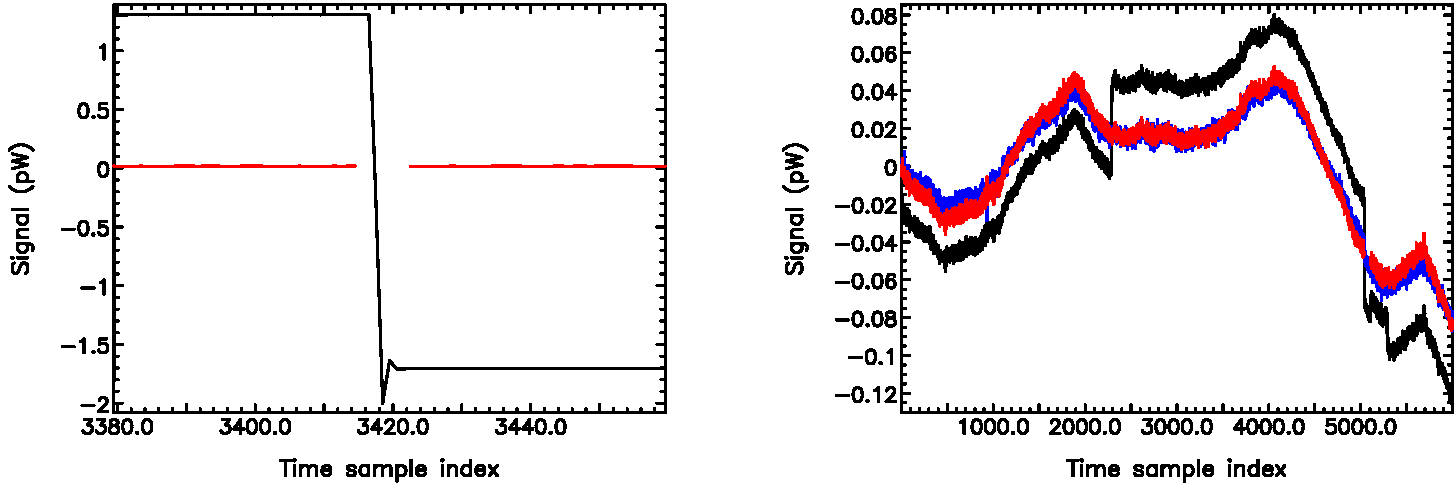
\includegraphics[width=\linewidth]{steps1.pdf}
\caption{Examples of steps in time series data. Steps occur with a wide
range of heights from the large steps shown on the left to the small
steps shown on the right. Large steps are often followed by a brief
``over-shoot'' as shown on the left. In both plots, the black curve is
the uncorrected time series, and the red curve is the corrected time
series. Samples close to a step are omitted in the corrected time series.
In the right hand plot, the blue curve is the uncorrected time series for
a nearby bolometer. The similarity between the red and blue curves shows
that the step correction is performing well.
}
\label{fig:steps1}
\end{figure*}

Sudden steps can occur in the time stream data from each bolometer.

\emph{why?}

The black curves in Fig.~\ref{fig:steps1} show examples of such steps in
the time streams for two bolometers. If not removed, these steps can
cause severe ringing in the FLT model (Section~\ref{sec:flt}) and visible
streaks in the final map, corresponding to the paths of individual
bolometers over the sky.

Steps occur with a wide range of heights and shapes. The ratio of step
height to noise can vary from less than 10 to several hundred. Some steps
occur over a single sample such as the step close to sample 5000 in the
right-hand plot of Fig.~\ref{fig:steps1}, but others happen more
gradually such as the step close to sample 5300. In addition, a step can
be preceded or followed by a short period of instability, as is visible
at the bottom of the step in the left hand plot of
Fig.~\ref{fig:steps1}. Further problems are caused by steps that occur
close together in time, such as the large downward step followed by a
smaller upward step close to sample 5000 in the right hand plot of
Fig.~\ref{fig:steps1}.

Detecting and correcting such a wide variety of steps reliably has proved
to be a challenge. The current step-correction algorithm is described in
detail in appendix~\ref{appendix:steps}. In outline, the following stages
are involved in detecting steps in a single bolometer time stream:

\begin{enumerate}
\item Median smooth the whole time stream.
\item Find the gradient of the median smoothed time series at each sample.
\item Smooth the gradient values to determine the local mean gradient and
subtract this local mean from the total gradient to get residual gradients.
\item Find residual gradient values that exceed 25 times the local RMS of
the residual gradients.
\item Group these high residual gradients into contiguous blocks of
samples.
\item Merge blocks that are separated by less than 100 samples
\end{enumerate}

The above process produces a list of candidate steps in each bolometer
time series. Each candidate step is then verified, measured and corrected
using the following procedure:

\begin{enumerate}

\item The above process can mis-interpret the edges of a bright source
as a step. So we ignore blocks that occur close to bright sources.

\item If the block passes the above test, a least squares linear fit is
performed to the median-filtered bolometer data just before the block, and
this fit is extrapolated to predict the data value expected at the centre
of the block on the basis of the preceding data.

\item A least squares linear fit is performed to the median-filtered
bolometer data just after the block, and this fit is extrapolated to
predict the data value expected at the centre of the block on the basis
of the following data.

\item The difference between these two expected data values is taken as
the step height.

\item The preceding three steps are repeated several times, each time
including a different selection of samples in the two least squares fits.
The mean and standard deviation of the corresponding set of step heights
is found.

\item If the mean step height is small compared to the standard deviation
of the step heights, or compared to the noise in the bolometer data, then
the step is ignored.

\item If the above checks are passed, all subsequent bolometer samples are
corrected by the mean step height.

\item Bolometer samples within the duration of the step, and a few
samples on either side, are flagged as unusable.

\end{enumerate}

Once all steps have been corrected within a bolometer time stream, a
constant value is added to all samples in the time stream to restore its
original mean value.

The results of step correction are shown by the red curves in
Fig.~\ref{fig:steps1}. For comparison, the blue curve shows the
uncorrected time stream from a nearby bolometer that does not suffer from
steps. The agreement between the red and blue curves confirms that
the step correction algorithm is working satisfactorily.


\subsubsection{Gap filling / apodization}
\label{sec:gaps}

The evaluation of the FLT model (Section~\ref{sec:flt}) involves taking
the Fast Fourier Transform of each bolometer time series. Data that has
been flagged as bad for any reason (for instance, due to the presence of
spikes, steps, or unusual common-mode signal) needs to be excluded from
this FFT. Two method are available:

\begin{itemize}
\item Gap-filling: each contiguous block of bad data samples is filled
with artificial data before taking the FFT. A least squares linear fit is
performed to the 50 samples preceding the block, and a similar fit is
performed to the 50 samples following the block. These are used to
estimate the expected values at the start and end of the block of bad
values. The bad values are then replaced by linear interpolation between
the expected start and end values. Gaussian noise is added with a
standard deviation equal to the mean of the RMS residuals in the two
fits.
\item Masking: each bad data value is replaced by zero, and an associated
mask is created that holds 1.0 for each good sample in the time stream and
0.0 for each bad sample. The masked data and the mask are then each filtered
in the same way using FFTs, and the filtered data is finally normalised by
dividing it by the filtered mask.
\end{itemize}

In addition to replacing bad samples before the FFT, it is also necessary
to ensure that the data values at the start and end of the time series
are similar. Since a Fast Fourier transform treats the data as a single
cycle in an infinitely repeating waveform, any large difference between
starting and ending value will effectively introduce sudden steps at the
start and end of each cycle, causing unwanted oscillations (ringing) in
the transform. Another consequence of the cyclic nature of the FFT is
that features at one end of the time series can affect the filtered
values at the other end of the time series. Two methods are available to
avoid these two problems:

\begin{itemize}
\item Apodisation: a number of samples at the start and end of each
bolometer time series are multiplied by a cosine function in order to
roll the data values off smoothly to zero. The default number of samples
modified at each end of the time series is given by half the ratio of the
sampling frequency to the lowest retained frequency. In addition, each
end of the time stream is padded with double this number of zeros. This
method is illustrated in Fig.~\ref{fig:pad2}.

\begin{figure}
\centering
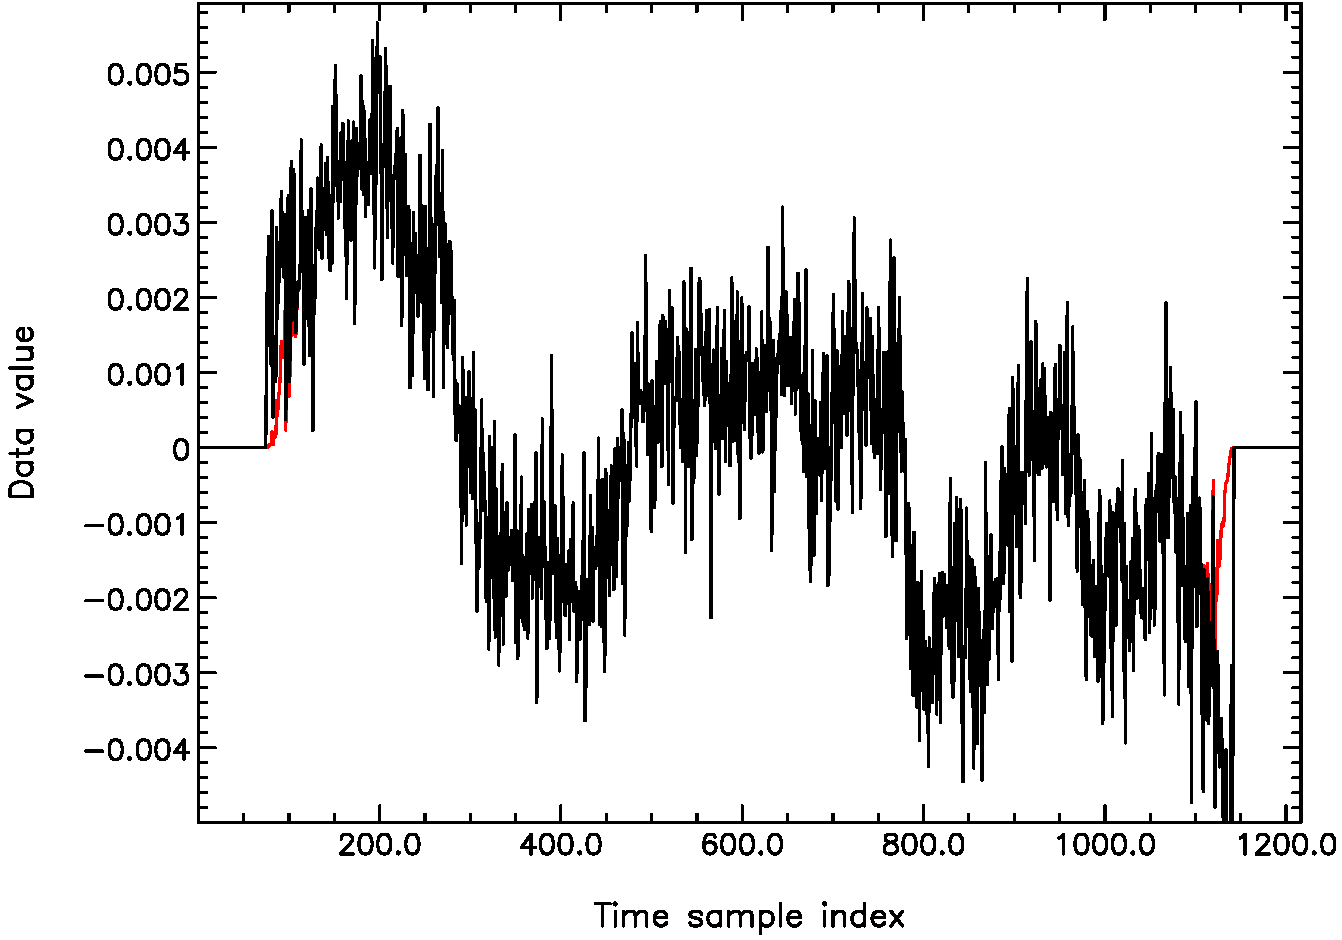
\includegraphics[width=\linewidth]{pad2.pdf}
\caption{The black curve shows a bolometer time stream, padded
with zeros. The red curve shows the time stream after apodisation.}
\label{fig:pad2}
\end{figure}

\item Padding with artificial data: instead of padding with zeros, each
time stream is padded with artificial data that connects the two ends of
the data stream smoothly and includes Gaussian noise. No apodisation is
performed. The number of samples of padding at each end is again equal to
the ratio of the sampling frequency to the lowest retained frequency.
This is illustrated in Fig.~\ref{fig:pad1}.

\begin{figure}
\centering
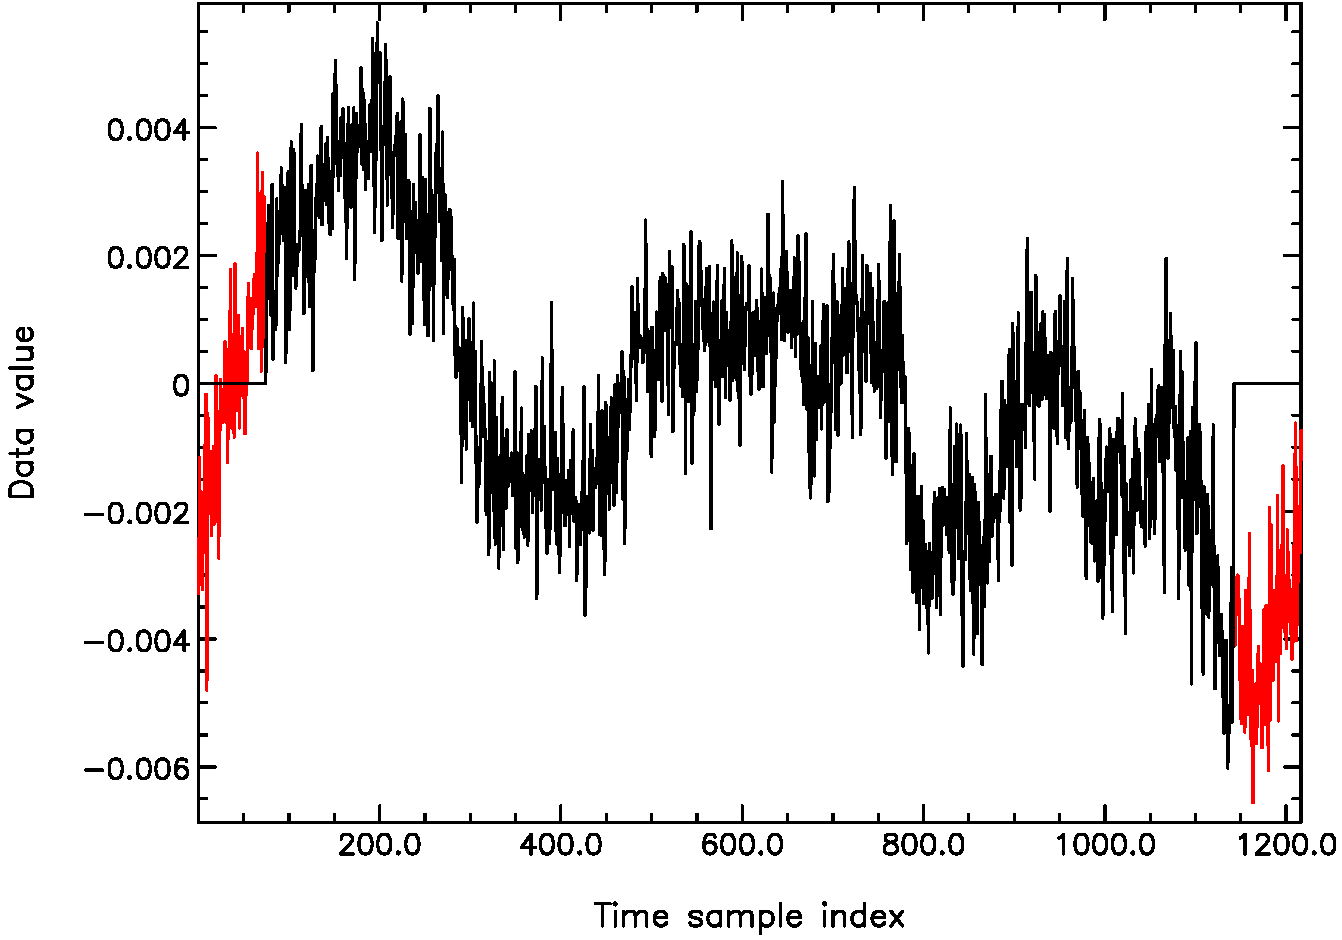
\includegraphics[width=\linewidth]{pad1.pdf}
\caption{The black curve shows the same bolometer time stream as in
Fig.~\ref{fig:pad2}, againpadded with zeros. The red curve shows the time stream
after padding with artificial data.}
\label{fig:pad1}
\end{figure}

\end{itemize}

\emph{Should reference CMB literature -- in particular look at
\citet{stompor2002}}.

\subsubsection{Flatfields}
\label{sec:flatfields}

TJ

Discuss heater ramps, normalizing off the common-mode signal
amplitude, astronomical sources, and the internal flatfield source.

\textit{Surely flatfields are discussed in the main \scuba\ paper so
don't really have any useful purpose here since they aren't
technically part of the map-maker.}

\subsubsection{Additional bad bolometer rejection}

TJ

Measuring the noise power spectra and throwing away outliers. Data
flagged bad by the DA system.

\subsubsection{Map-based despiking}
\label{sec:mapdespike}

It is possible to use the map estimate (Section~\ref{sec:ast}) to
provide additional despiking of the time-series. Unlike the
time-domain despiker (Section~\ref{sec:timedespike}), this calculation
uses the scatter in the population of samples used to estimate the map
pixel values (from different times and bolometers) to reject
outliers. This method is more robust against false-positive detections
of bright/compact astronomical sources since transient features in the
time-series are unlikely to occur by chance whenever a bolometer
crosses a specific location on the sky, whereas real astronomical
sources are at fixed spatial locations.

The estimated variance, $\mathbf{v_p}(x_i,y_i)$, of the normalized
weighted samples that land in the $i$th map pixel is simply the biased
weighted sample variance (i.e., the variance map value multiplied by
the number of samples)
%
\begin{equation}
  \mathbf{v_p}(x_i,y_i) = N_i \mathbf{v}(x_i,y_i).
\end{equation}

In order to compare the weighted \emph{differences} between the
samples and the map values, [$\mathbf{b}_j - \mathbf{m}(x_i,y_i)$] to
$\mathbf{v_p}$, they must be scaled appropriately. We define a
normalized difference, $\mathbf{d}_j$, in such a way that the variance
of this new variable gives the weighted sample variance of the
underlying data points,
%
\begin{eqnarray}
  \frac{\sum_j \mathbf{d}_j^2}{N} &=&
  \frac{\sum_j \mathbf{w}_j [\mathbf{b}_j - \mathbf{m}(x_i,y_i)]^2}
       {\sum_k \mathbf{w}_k} \\
   \Rightarrow \mathbf{d}_j^2 &=& \frac{N \mathbf{w}_j [\mathbf{b}_j -
       \mathbf{m}(x_i,y_i)]^2}{ \sum_k \mathbf{w}_k} .
\end{eqnarray}
%
The map-based despiker flags those $\mathbf{d}_j$ that are further
than some threshold number of standard deviations,
$\sqrt{\mathbf{v_p}}$, away from zero so that they are not used in
subsequent iterations.


%------------------------------------------------------------------------------
\section{Examples}
\label{sec:examples}
%------------------------------------------------------------------------------

In this section three different common types of data are reduced: a
bright point source, Uranus (Section~\ref{sec:point}); a bind survey
of high-redshift galaxies in the Lockman Hole
(Section~\ref{sec:cosmo}); and a map of a bright extended star-forming
region in our Galaxy, M17 (Section~\ref{sec:extended}). In each case,
variations on the default algorithm from Section~\ref{sec:algorithm}
are described.

%-------------------------------------------------
\subsection{Known point source}
\label{sec:point}
%-------------------------------------------------

The accurate measurement of positions and brightnesses of known point
sources are necessary in real-time to establish telescope pointing
offsets and focus. They are also necessary to measure the FCF
(absolute calibration), and hence noise performance of the instrument
in astronomical units.  In this example we produce a 450\,\micron\ map
of Uranus (observation 26 on 20111017), which is a nearly point-like
source for \scuba\ that is commonly used as a primary flux
calibrator. The now standard CV daisy scan pattern was used, with a
scan speed of 155 arcsec\,sec$^{-1}$. We perform several different
reductions of the data to illustrate the purpose of different model
components and the convergence properties of the solution
(Fig.~\ref{fig:pointmaps}). In all cases the maps are produced on a
grid of azimuth (horizontal) and elevation (vertical) offsets from the
position of Uranus (the origin), using 2\,arcsec pixels.

The first, simplest reduction of the data uses only the \model{COM}
model to estimate and remove the common-mode signal in order to
suppress low-frequency noise in the data. After \model{COM}, the
extinction correction is applied (\model{EXT}), and an initial map is
estimated using equal weighting for all of the detectors. This
estimate of \model{AST} is then removed from the data, and the noise
is measured in the residuals to estimate weights for the subsequent
and final iteration. The resulting map after these two iterations is
shown in Fig.~\ref{fig:pointmaps}a. While the S/N of Uranus is clearly
large ($\sim$250 as estimated by SMURF), enabling us to see the faint
sidelobes (circle and cross pattern), the map also has obvious
circular streaks and other large-scale ripples. The circular streaks
are due to the fact that \model{COM} does not account for all of the
low-frequency noise (see Fig.~\ref{fig:pspec}), and therefore each
bolometer leaves a trace of the circular scan pattern in the map as
each of their baselines slowly drift independently. A significant
contribution to the larger-scale ripples in the map, however, can be
made by degeneracies in the map solution as we discuss below.

To illustrate how large-scale ripples can form (and grow), the same
map solution is run for 100 iterations and shown in
Fig.~\ref{fig:pointmaps}b, now exhibiting a strong vertical
gradient. The degeneracy is easy to understand if the time-domain
behaviour of each model component is considered. The top panel of
Fig.~\ref{fig:degeneracy} shows the residual signals for a single
bolometer after 2 (black) and 100 (grey) iterations which are nearly
identical, yet the \emph{change} in the estimated \model{COM} (green)
and \model{AST} (red) signals between 2 and 100 iterations are
large. However, it is also clear that the estimated \model{COM} and
\model{AST} signals are \emph{complimentary}. In other words, the
large change in the \model{AST} signal is cancelled by freedom in the
\model{COM} signal to grow with opposite sign. For comparison, the
bottom panel of Fig.~\ref{fig:degeneracy} shows the pointing solution
for this section of data, and the shapes of the \model{AST} and
\model{COM} signals match the elevation component, which is aligned
with the gradient in Fig.~\ref{fig:pointmaps}b. Generically, the
calculation of \model{COM} will remove any information on angular
scales that are larger than the array footprint (outline shown in
Fig.~\ref{fig:pointmaps}b for reference), meaning that the map
solution is unconstrained on such large scales.

One improvement is to simply restrict the low-frequency signal that
goes into the maps by applying a high-pass filter to the bolometer
time-series. A third reduction of the data uses the default map-making
parameters, as described in Section~\ref{sec:algorithm}, which adds
the \model{FLT} model to accomplish this task immediately prior to map
estimation. We set the filter edge based on an angular scale of
200\,arcsec, which, given the scan speed of 155\,arcsec\,sec$^{-1}$,
corresponds to a frequency of 0.78\,Hz. Now using the automatic
map-based convergence test (Section~\ref{sec:converge}), the resulting
map converges after 10 iterations (Fig.~\ref{fig:pointmaps}c). Both
the circular streaks and the large-scale gradient are now removed, but
they have been replaced by an obvious, circularly-symmetric ringing
pattern about Uranus. The reason for this ringing is that the
hard-edged high-pass filter in frequency space is equivalent to a
$\sinc$ function-like response in map space. Since the scan pattern is
isotropic (scans equally at all position angles), and there is a
bright point-like source, the result is an azimuthally-symmetric
$\sinc$ function-like pattern in the map. Note that due to the
iterative nature of the solution, much of the signal in the source is
actually removed for subsequent iterations of \model{FLT}, but as in
the previous case, degeneracies between the map and the \model{FLT}
and \model{COM} signal components can still lead to complicated
structures.

The preceding examples illustrate the need for constraints in the map
solution in many situations. For calibrators (and other previously
known bright, compact sources), a good, simple prior is to constrain
the map to a value of zero away from the known locations of
emission. In Fig.~\ref{fig:pointmaps}d, a map is produced in an
identical manner to the previous example, but now setting the map
explicitly to zero beyond a radius of 60\,arcsec from the location of
Uranus (much larger than the FWHM of the main lobe), for all but the
final iteration. In this case, the map converges after 6 iterations,
and all of the previous artifacts have been effectively removed. Since
the map is now flat away from the source, and constrained to a value
of zero, it is appropriate for performing aperture photometry
directly, with no need for an additional reference annulus. This
approach to constrained map-making is similar to that employed for
poorly cross-linked scans of compact (though resolved) sources by
\citet{wiebe2009} using BLAST data.

\begin{figure*}
\centering
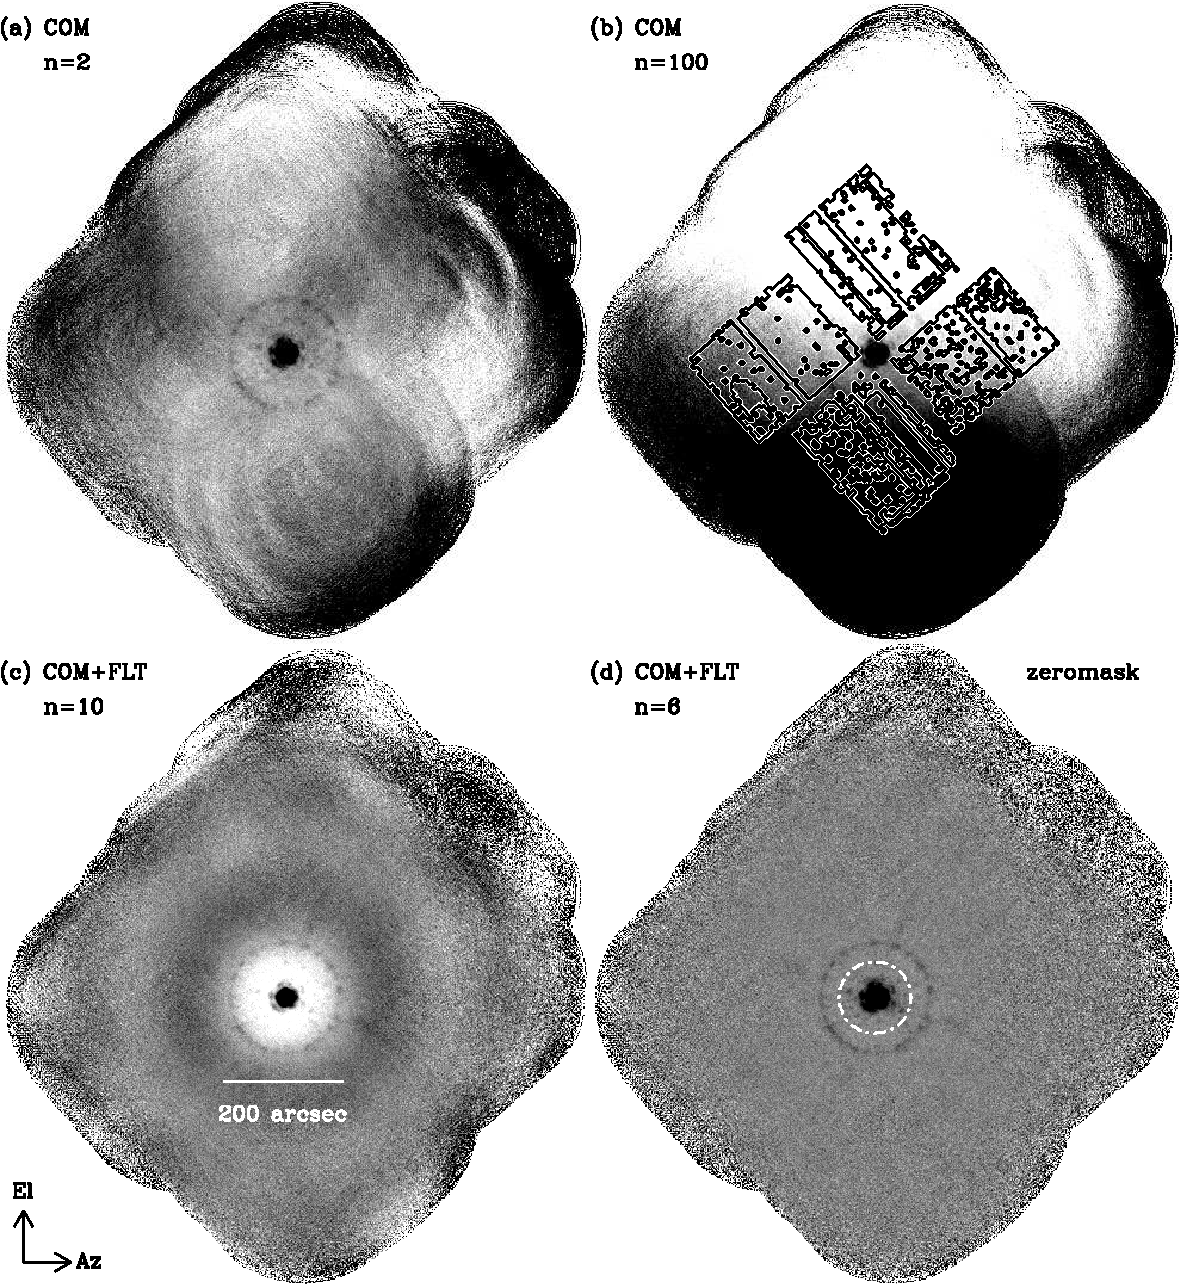
\includegraphics[width=\linewidth]{pointmaps.pdf}
\caption{Multiple reductions of a 450\,\micron\ daisy scan of Uranus,
  all scaled between -0.002\,pW (white) and +0.002\,pW (black): (a)
  Reduction in which only common-mode subtraction is used to suppress
  low-frequency noise, and the reduction is forced to use 2 iterations
  (after the first iteration an estimate of the source flux is
  removed, and the noise is measured in the residuals to obtain
  appropriate weighting for the second and final iteration) ---
  circular streaks are caused by independent low-frequency noise that
  is not removed by the common-mode (Uranus peak 0.15\,pW); (b) same
  as (a) but using 50 iterations, illustrating the degeneracy between
  large-scale structure and the common-mode (the footprint of working
  bolometers is also shown for reference, Uranus peak 0.15\,pW); (c)
  reduction in which high-pass filtering above 0.775\,Hz
  (corresponding to a spatial scale of 200\,arcsec as indicated) is
  applied after common-mode removal, but before the map estimate ---
  the map-based convergence test is activated and the solution halts
  after 10 iterations, but leaving large-scale ringing due to the
  filter (Uranus peak 0.27\,pW); (d) same as (c), but now the region
  of the map beyond the white dot-dashed circle is constrained to a
  value of zero until all but the final iteration --- the map is now
  extremely flat, there is little attenuation of the source flux, and
  the diffraction pattern is clearly seen (Uranus peak 0.27\,pW).}
\label{fig:pointmaps}
\end{figure*}

\begin{figure}
\centering
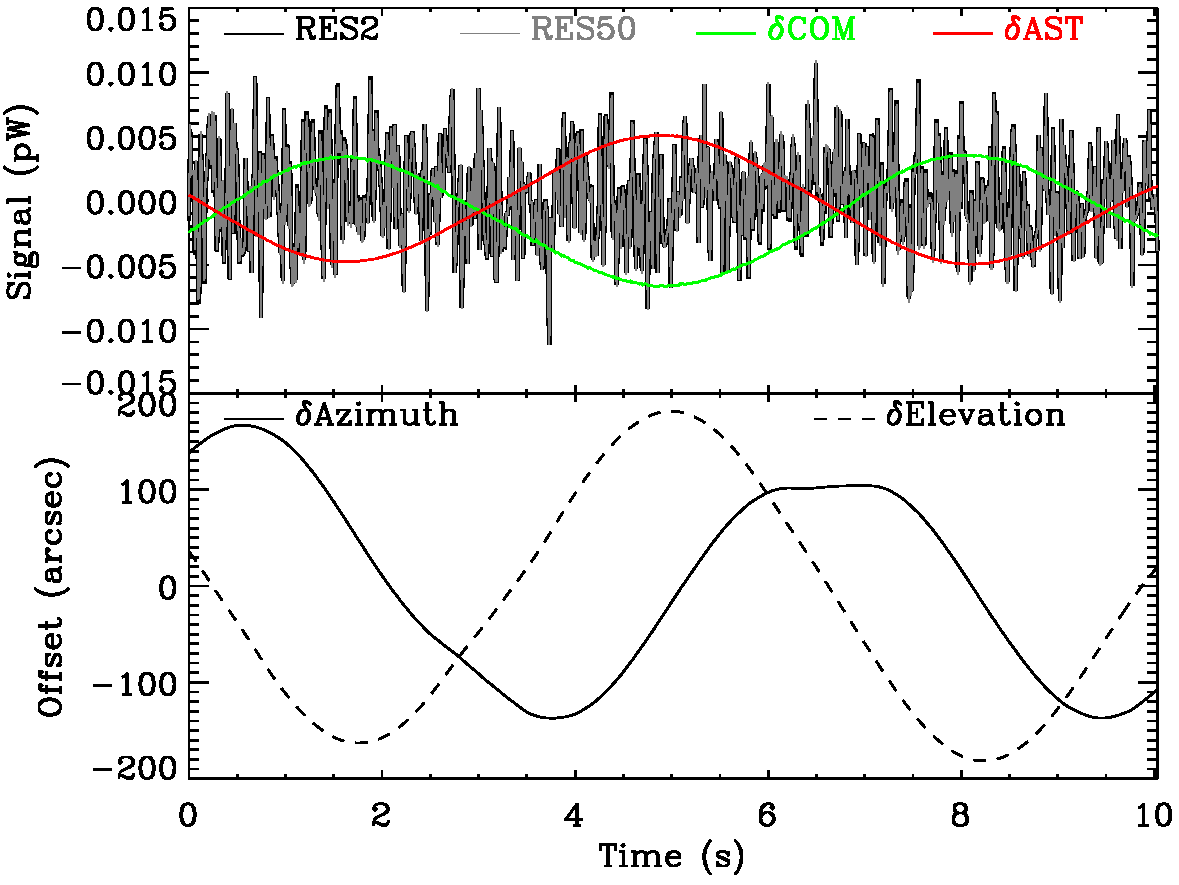
\includegraphics[width=\linewidth]{degeneracy.pdf}
\caption{Demonstration of the degeneracy between large-scale
  structures in the map and common-mode removal, corresponding to
  panels (a) and (b) in Fig.~\ref{fig:pointmaps}. The black and grey
  lines in the top panel show the residual signal for a single
  bolometer after 2 and 100 iterations respectively (they are nearly
  identical). The green and red lines show the \emph{difference}
  between the \model{COM} and \model{AST} (the signal produced by the
  current map estimate for a given bolometer) model components for
  that bolometer between iterations 2 and 100 respectively. This shows
  that a strong signal has grown over time, and it has equal but
  opposite signs in the two model components, so that they cancel one
  another. The bottom panel shows the scan pattern of the telescope
  over the same period; clearly the \model{COM}/\model{AST} model
  degeneracy is correlated with the elevation offset, and referring to
  Fig.~\ref{fig:pointmaps}, panel (b), this clearly corresponds to the
  strong vertical gradient that has appeared}.
\label{fig:degeneracy}
\end{figure}

%-------------------------------------------------
\subsection{Deep blind survey}
\label{sec:cosmo}
%-------------------------------------------------

\scuba\ surveys designed to detect extremely faint point-sources
(e.g. high-redshift star-forming galaxies, and debris disks) are
ideally limited by the white-noise performance of the instrument. The
approach described here for maximizing the S/N of point-sources
involves three major steps: (i) generating a map that removes most
low-frequency noise sources with approximately linear response,
without prior knowledge of the location of sources; (ii)
\emph{whitening} (essentially flattening) the map to make the noise
properties of the map easier to deal with; and (iii) detecting point
sources using a \emph{matched-filter}. Note that variations on this
general procedure have been used extensively in the submm cosmology
community using previous instruments
\citep[e.g.][]{scott2002,laurent2005,coppin2006,scott2008,perera2008,devlin2009}.
In this section we will reduce scans of the Lockman Hole taken during
S2SRO as a pilot project for the Cosmology Legacy Survey. It consists
of $\sim8.5$\,hours of data taken in 36 separate scans (average
15\,min. each) spread over February and March 2010, covering an area
of about 50\,arcmin$^2$. The full list of dates and observation
numbers includes 20100218: 63, 64, 65, 70, 71, 72, 90, 91, 92, 97, 98,
99; 20100220: 111, 112, 113, 118, 128, 129, 130; 20100303: 61, 62, 64,
69, 70, 72, 73, 74, 75; 20100309: 87, 88, 90, 91; and 20100311: 59,
64, 65, 72. These observations represent about 80\% of the total data
taken as part of the project; the remaining observations were dropped
due to problems keeping the arrays properly locked during S2SRO, and
were easily identified by their highly variable and erratic bolometer
time-series (which resulted in maps full of large streaks).


\begin{figure*}
\centering
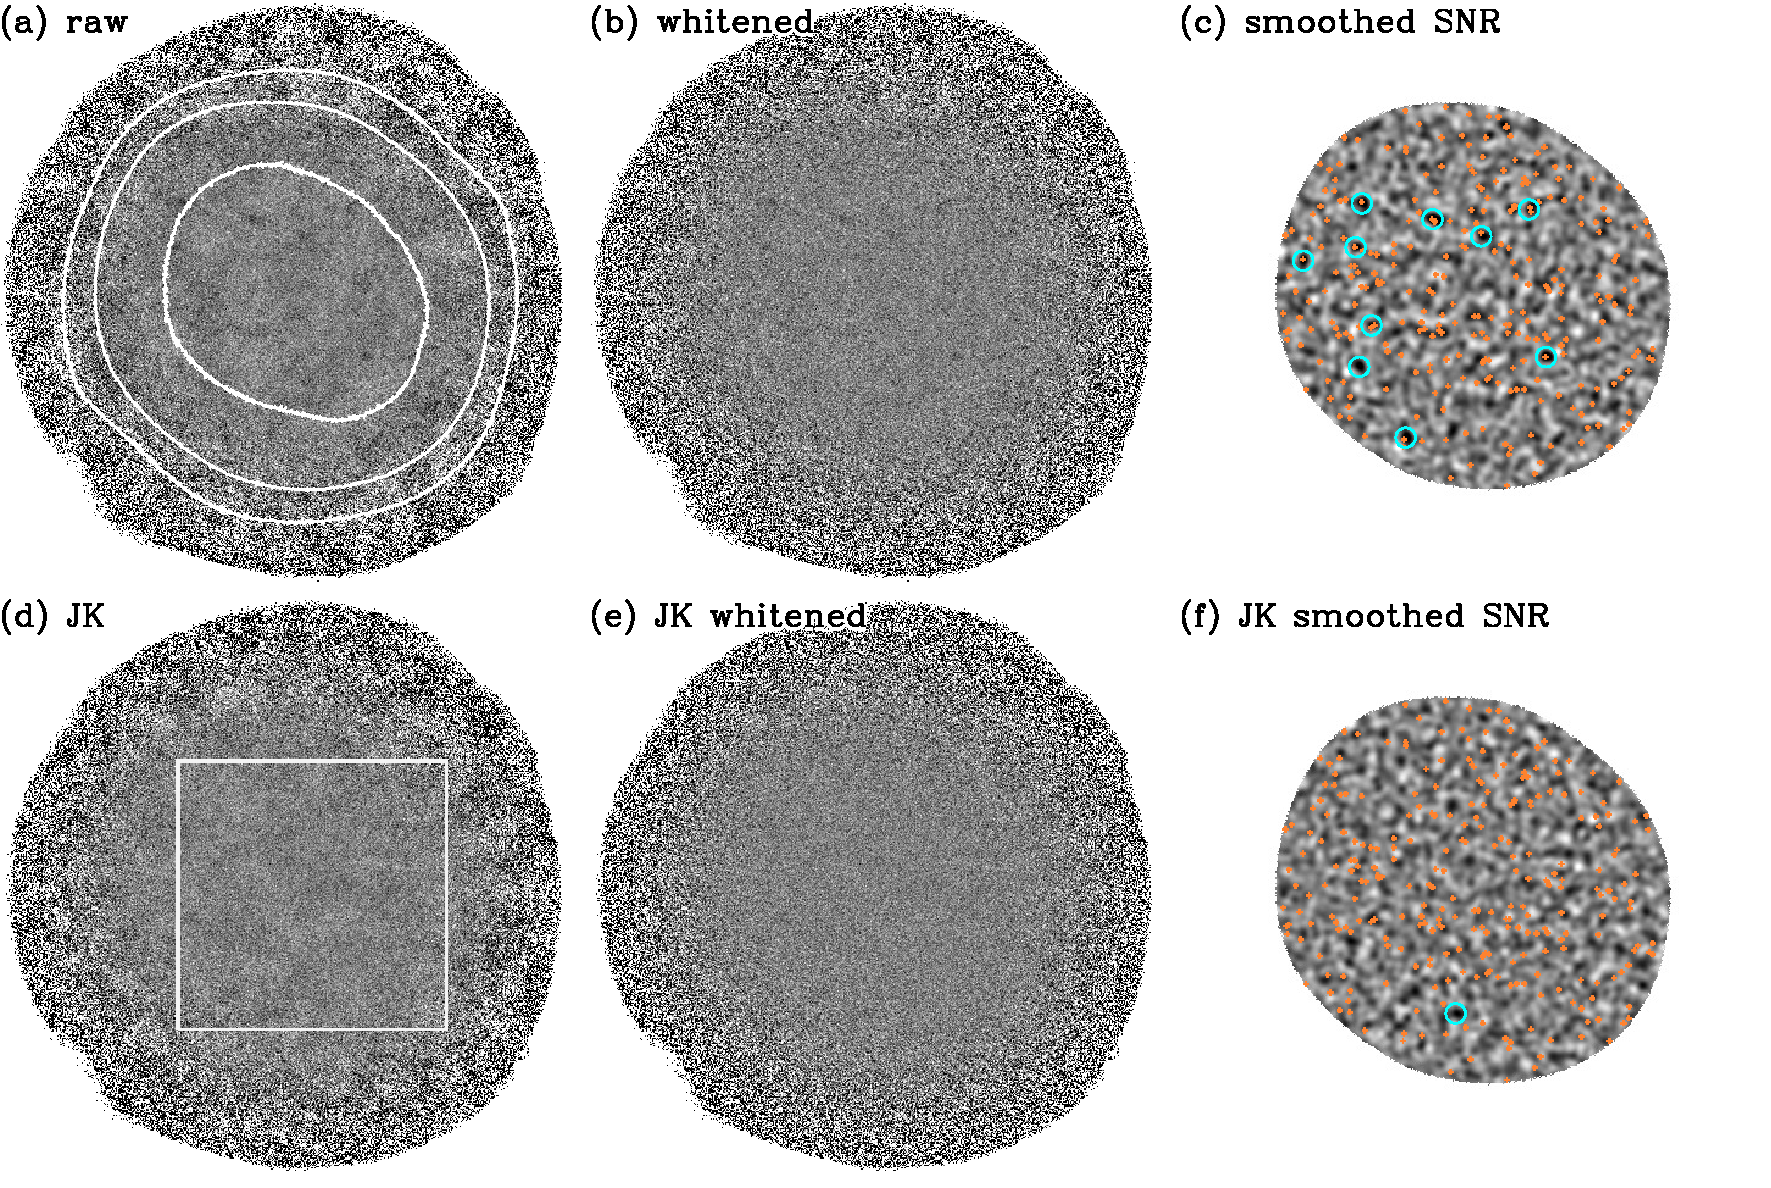
\includegraphics[width=\linewidth]{lockman_maps.pdf}
\caption{Reduction of a blank-field survey: the Lockman Hole. (a) raw
  output of SMURF using high-pass filtering as a pre-processing step,
  followed by 4 iterations using only the \model{COM} model to remove
  residual low-frequency noise. White contours correspond to estimated
  noise levels of 1.25, 2.5 and 5.0 times the minimum noise at the
  centre of the map. (b) the whitened map using a filter based on the
  angular power spectrum of the jackknife map. (c) The whitened map
  cross-correlated with the whitened PSF to identify point sources
  [restricted to a lower-noise region, within the area denoted by the
  second contour of panel (a)]. The image shows the S/N, with
  3.8-$\sigma$ peaks indicated with blue circles (radius
  8\,arcsec). The orange ``$+$'' signs show the locations of 1.4\,GHz
  radio sources from \citet{owen2008} with $S\gsim15$\,$\mu$Jy. Of the
  10 submm peaks, 9 are within this search radius of at least one
  radio source. (d) jackknife map produced from the difference of two
  maps, using the even and odd scan numbers, respectively. Provided
  that all noise sources are statistically un-correlated between the
  two halves of the data, the map is a plausible realization of the
  noise without contamination from astronomical sources. (e) The
  jackknife map whitened using the same filter as that in panel
  (b). The whitened jackknife map cross-correlated with the same
  whitened PSF as in panel (c). Again, orange ``$+$'' and blue circles
  indicate radio sources and 3.8-$\sigma$ peaks, respectively. Unlike
  panel (c), there is only a single significant peak, and it is not in
  the vicinity of a radio source.}
\label{fig:lockman_maps}
\end{figure*}

The first step, map generation, is different from that described in
Section~\ref{sec:point} in two key ways. Since the locations of
sources are unknown \emph{a priori}, a map constraint is not
employed. Large-scale diverging structures in the map must be
mitigated, and the method used in this example (the default processing
in SMURF) is to apply a high-pass filter to the data \emph{once} as a
pre-processing step. The iterative solution is then run using only
\model{COM}, \model{EXT}, \model{AST}, and \model{NOI}. In other
words, there is no information in the bolometer signals below some
cutoff frequency, and residual correlated high-frequency noise above
the cutoff is only removed through iterative common-mode
subtraction. The map is shown in Fig.~\ref{fig:lockman_maps}a. The
map-maker has been tested in two ways: (i) large numbers of iterations
are used to verify that the maps converge without the growth of large
structure; and (ii) adding synthetic sources to the data at a range of
brightnesses verify that the map-maker response to them is
\emph{linear} (i.e. the relative shape and amplitude compared to the
input source is independent of brightness). The response to a
synthetic point source (solid line) after map-making (dotted line) is
shown in Fig.~\ref{fig:lockman_psf}. Clearly the use of a high-pass
filter as a pre-processing step, and having no other map-constraints,
has the down-side of introducing sidelobes around the main
peak. However, the way this filter affects point-sources is both
well-known, and linear.

\begin{figure}
\centering
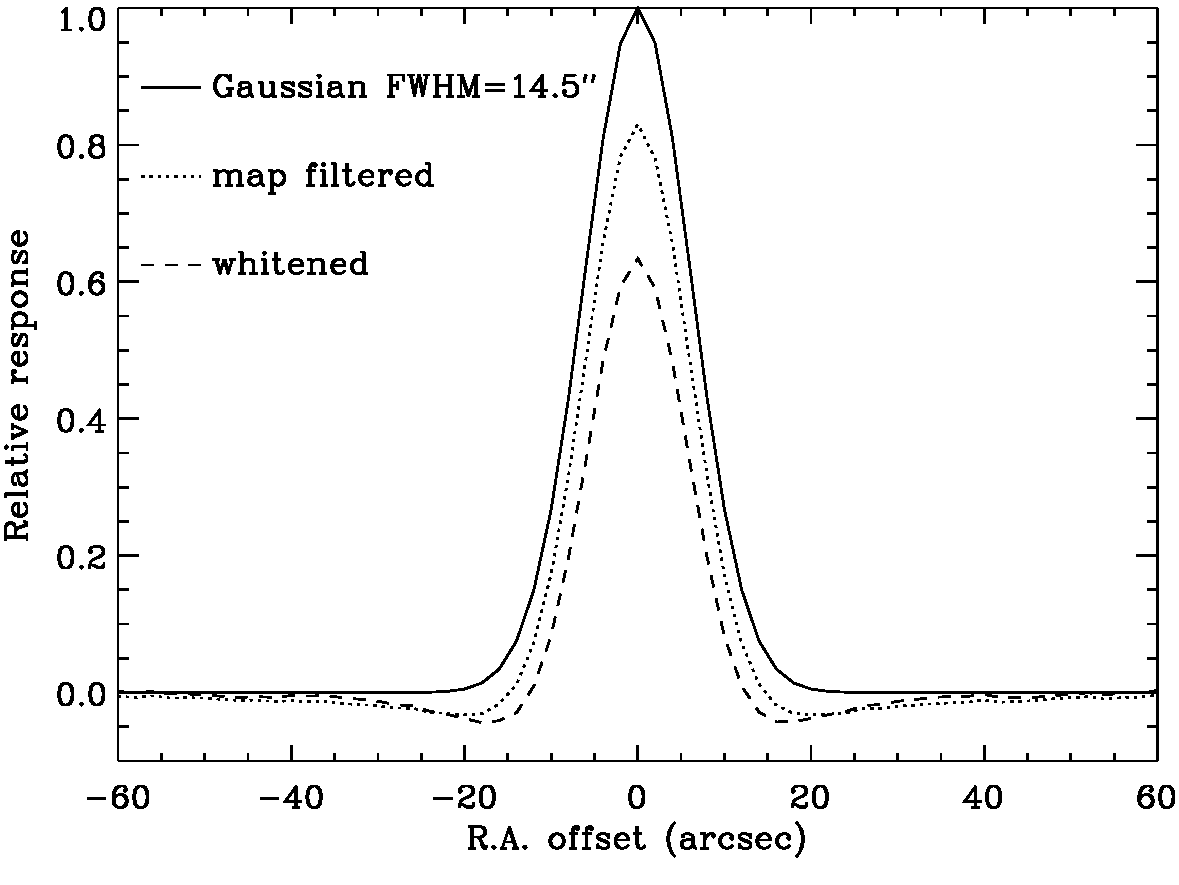
\includegraphics[width=\linewidth]{lockman_psf.pdf}
\caption{Slice through the angular response to an ideal Gaussian point
  source (solid line) along the R.A. axis following map-making using
  the default blank-field processing with SMURF (dotted line), and
  upon application of the whitening filter (dashed line). The ``map
  filtered'' response is produced by adding the ideal Gaussian to the
  real data near the centre of the Lockman Hole map, and re-reducing
  the data. The resulting dotted line gives the expected shape of a
  source in panel (a) from Fig.~\ref{fig:lockman_maps}. Applying the
  whitening filter (reciprocal of the solid orange line in
  Fig.~\ref{fig:lockman_pspec}) to the dotted line gives the whitened
  line, which is the expected shape of a source in panel (b) from
  Fig.~\ref{fig:lockman_maps}. Finally, cross-correlating the whitened
  map with this whitened PSF is an effective ``matched filter'' for
  identifying point-like sources, and this smoothed map is shown in
  panel (c) of Fig.~\ref{fig:lockman_maps}.}
\label{fig:lockman_psf}
\end{figure}

%... high-pass
%filter + iterative common-mode removal takes place of PCA cleaning in
%AzTEC reduction ... probably more linear.

Even though the map looks quite flat, there is a mixture of faint
astronomical sources, and what is probably residual low-frequency
noise causing faint ripples visible to the naked eye. Since the
mixture of the two components is unknown, the first step is to
suppress the low-frequency noise, under the assumption that such
contaminants occur randomly in time, while astronomical sources are
(usually) constant.

First, the angular power spectrum of noise is estimated from a
\emph{jackknife map}: maps are produced from two independent halves of
the total data set, and the jackknife signal in a map pixel,
$S_\mathrm{JK}$, and its variance, $\sigma^2_\mathrm{JK}$ are
estimated from the two input map fluxes, $S_1$, $S_2$, and the
corresponding variances, $\sigma^2_1$, and $\sigma^2_2$ as,
%
\begin{eqnarray}
S_\mathrm{JK} = \frac{S_1 - S_2}{2} \\
\sigma^2_\mathrm{JK} = \frac{\sigma^2_1 + \sigma^2_2}{4}.
\end{eqnarray}
%
Provided that the noise in one half of the data is uncorrelated with
that from the other half, the signal in the jackknife map should
resemble noise drawn from the same parent distribution as that of the
real map. The astronomical signal, however, should be cleanly removed
(provided that there are no strong time-varying signals, and also
assuming that errors due to calibration between the two halves are
insignificant). The approach we have taken to minimize systematics is
to produce the two maps using odd and even scan numbers (i.e., each
map will contain a nearly evenly-spaced sampling of data across the
full dataset).

Since the \scuba\ scan strategy is usually isotropic (all position
angles scanned with roughly equal weights), we make the simplifying
assumption that the angular noise power spectrum is azimuthally
symmetric. For these data, there are no obvious anisotropic structures
in the 2-dimensional FFT. The radial (azimuthally-averaged) angular
power spectrum therefore encodes all of the useful information about
the noise properties. These power spectra for the raw output of SMURF,
and the jackknife map (transforming only the approximately uniform
region indicated by the square in Fig.~\ref{fig:lockman_maps}d in each
case) are shown by the dashed black, and solid orange lines in
Fig.~\ref{fig:lockman_pspec}, respectively. Both power spectra are
approximately flat at spatial frequencies $\gsim 0.06$\,arcsec$^{-1}$
(scales $\lsim16$\,arcsec), with the exception of a line at
$\sim0.175$\,arcsec$^{-1}$ (a scale of $\sim5.7$\,arcsec). A theory
for this feature is that it is related to the inter-bolometer spacing
in the focal plane (which happens to be this size): small relative
drifts in the baselines of adjacent bolometers may produce faint
parallel stripes in the map along the scan direction (the
superposition of many scans at different angles then results in an
isotropic noise pattern). It is not likely that this signal is due to
astronomical sources because it appears with a nearly equal amplitude
in both the real map and the jackknife.  At lower spatial frequencies,
both the real map and the jackknife power spectra grow significantly,
as a result of the more obvious large-scale undulations in
Figs.~\ref{fig:lockman_maps}(a) and (d).

\begin{figure}
\centering
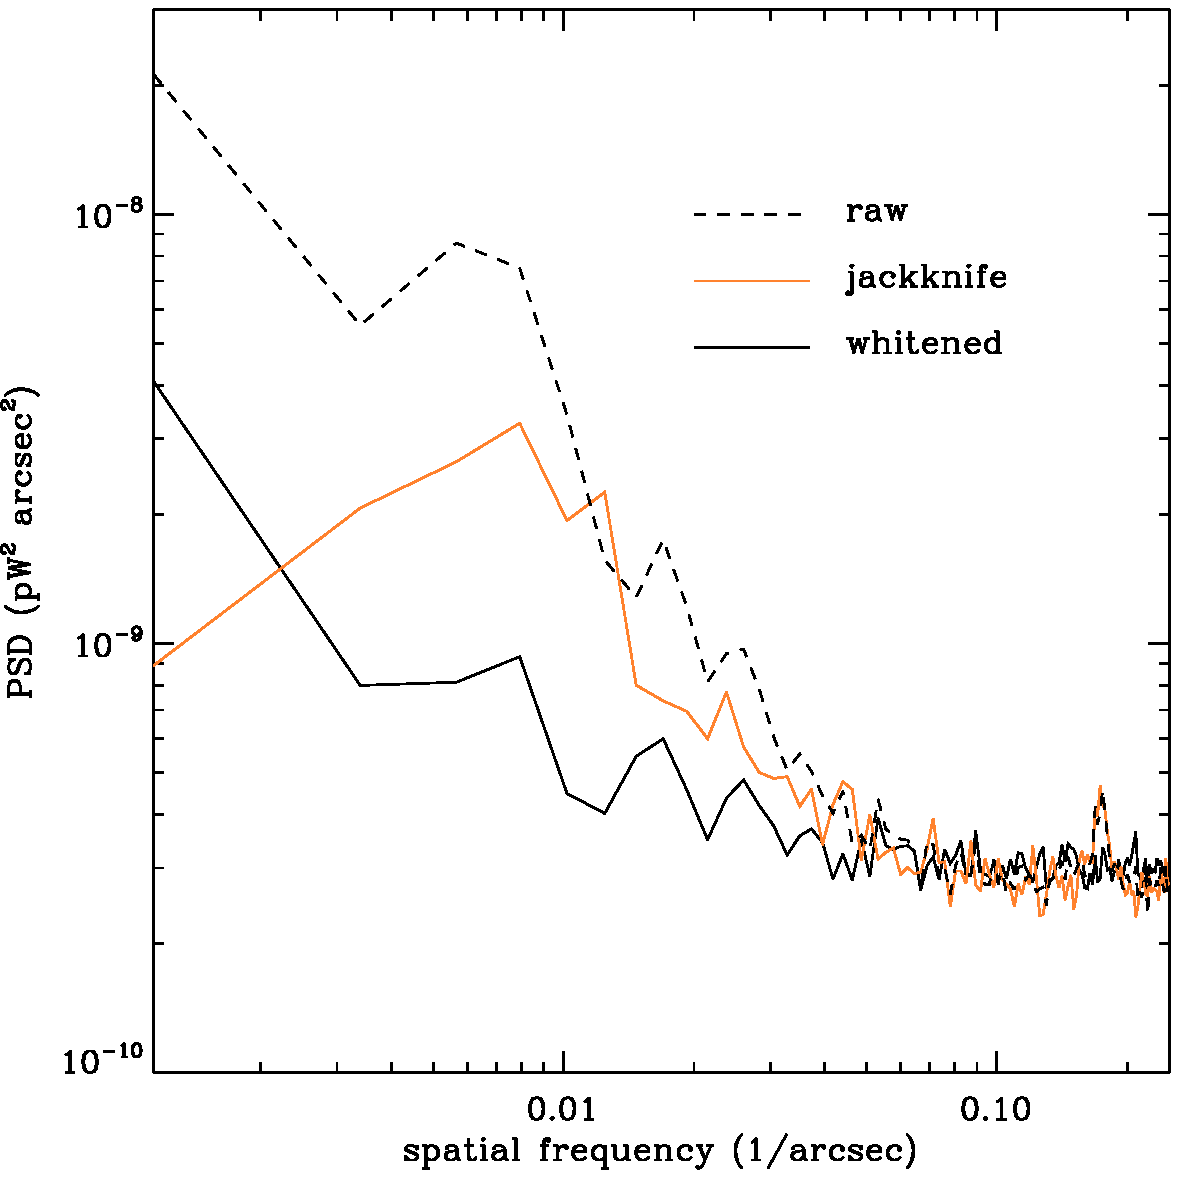
\includegraphics[width=\linewidth]{lockman_pspec.pdf}
\caption{Radial (azimuthally-averaged) angular power spectral
  densities for the raw map output by SMURF (dashed black line), the
  jackknife (solid orange line), and whitened (solid black line) maps
  (panels (a), (d), and (b) from Fig.~\ref{fig:lockman_maps},
  respectively (considering only the square region indicated in
  Fig.~\ref{fig:lockman_maps}d). Since the raw map contains spatially
  correlated signals on large scales both due to noise and
  astronomical signals (low-spatial frequencies), the jackknife map
  (difference of two approximately equal-length subsets of the data)
  is used to generate a plausible realization of pure noise. Assuming
  that the noise properties are isotropic, a whitening filter is
  estimated from the reciprocal of the jackknife power spectrum with
  only a radial dependence. The power spectrum of the resulting signal
  map still has residual power on large scales, which is presumably
  due to astronomical sources.}
\label{fig:lockman_pspec}
\end{figure}

To suppress noise in the map, we construct a \emph{whitening filter}
from the reciprocal of the jackknife angular power spectrum (orange
line in Fig.~\ref{fig:lockman_pspec}), normalized by the white-noise
level estimated from the RMS power at angular frequencies $>
0.1$\,arcsec$^{-1}$. The filter is applied by scaling the power
spectrum of the map by this function, and then transforming back into
real space. The whitened map is shown in Fig.~\ref{fig:lockman_maps}b,
and for comparison, the jackknife map has also been whitened in
Fig.~\ref{fig:lockman_maps}e. In both cases, the maps are both
visually flatter than the non-whitened cases.

The angular power spectrum of the whitened signal map is shown with a
solid line in Fig.~\ref{fig:lockman_pspec}. At low angular frequencies
($\lsim 0.5$\,arcsec$^{-1}$) there is significantly less power than
the raw map. However, it also clearly has \emph{some} power in excess
of the white noise level. In theory, this residual signal is produced
by astronomical sources, although its origin cannot be determined from
this plot alone; nor are astronomical sources readily visible in the
map (Fig.~\ref{fig:lockman_maps}b. To identify sources, we next apply
a \emph{matched filter} to the whitened maps.

For blind, high-redshift surveys, individual sources are expected to
be un-resolved by the \scuba\ 7.5--14.5\,arcsec FWHM beams. Under this
assumption, cross-correlation between the map and the known PSF yields
the maximum-likelihood flux density of supposed point-sources centered
over every location in the resulting map \citep[an extremely
well-known result throughout astronomy, see][]{stetson1987}. Peak
identification in such smoothed maps have been used extensively in the
submillimetre community as both an efficient source-detection and
photometric measurement strategy. In terms of the angular power
spectrum, a matched-filter may also be thought of as an optimal
\emph{low-pass} filter, that suppresses noise on scales smaller (and
therefore higher angular frequencies) than the beam. For the case at
hand, the effective PSF for the whitened maps is given by the dotted
curve in Fig.~\ref{fig:lockman_psf}. Maps smoothed by this shape are
shown for the whitened signal, and jackknife maps in
Figures~\ref{fig:lockman_maps}c and f respectively. Note that these
images are plotted in SNR units, where the smooth noise maps have been
calculated by propagating the original noise maps output by SMURF both
through the whitening and matched filters (each of which are linear
operations).

Have real astronomical sources been detected using the matched-filter?
For both the smoothed signal and jackknife maps, orange circles denote
3.8-$\sigma$ peaks. While not justified here, this threshold is fairly
typical for other ground-based submillimetre surveys in recent years
\citep[e.g.,][]{coppin2006,perera2008,weiss2009} leading to estimated
false-identification rates of order $\sim$5\%, and is chosen here as a
convenient reference. In the former, 10 peaks are found, whereas there
is only 1 in the latter. However, this test does not preclude the
possibility that some correlated noise made it into the jackknife
map, in which case the estimated SNRs are misleading.

One simple test of the calculated noise properties is to compare the
signal and jackknife SNR distributions with ideal Gaussians. The top
panel of Fig.~\ref{fig:lockman_hist} shows the whitened (but not match
filtered) signal (blue) and jackknife (histograms), along with a
Gaussian (mean 0, standard deviation 1, and area normalized to the
number of map pixels) as a dashed line. In this case, it is clear that
the SNR distributions for both maps are nearly indistinguishable from
the theoretical distribution of white noise. This result shows us
that: (i) the whitening filter appears to have removed correlated
large-scale noise since the jackknife map histogram is consistent with
white noise; and (ii) any potential astronomical signals are small
compared to the typical white noise in most map pixels (unsurprising
given the appearance of Fig.~\ref{fig:lockman_maps}b). Next, we
examine the SNR histograms for maps processed with the matched filter
in the bottom panel of Fig.~\ref{fig:lockman_hist}. Again, the
histogram of the jackknife SNR data appears consistent with pure
noise. However, the signal map now deviates significantly from a
Gaussian distribution, with a clear \emph{positive} tail (as one would
expect for emitting sources). In fact, integrating the positive tails
beyond our 3.8-$\sigma$ source-detection threshold (vertical solid
line) yields 229 map pixels in the signal map, compared with 3 in the
jackknife map (out of 80603 pixels in the entire region). Note that
given the small pixel size of the map, several pixels generally
contribute to each peak. Note that this procedure gives only a flavour
of the analysis that is usually required to produce a robust source
lists. Additional tests, along with a careful consideration of
completeness and false-positive rates usual require a series of Monte
Carlo simulations that are beyond the scope of this work. We direct
the interested reader to a selection of papers on the subject:
\citet{scott2002,coppin2006,perera2008,weiss2009} and
\citet{chapin2011}.

\begin{figure}
\centering
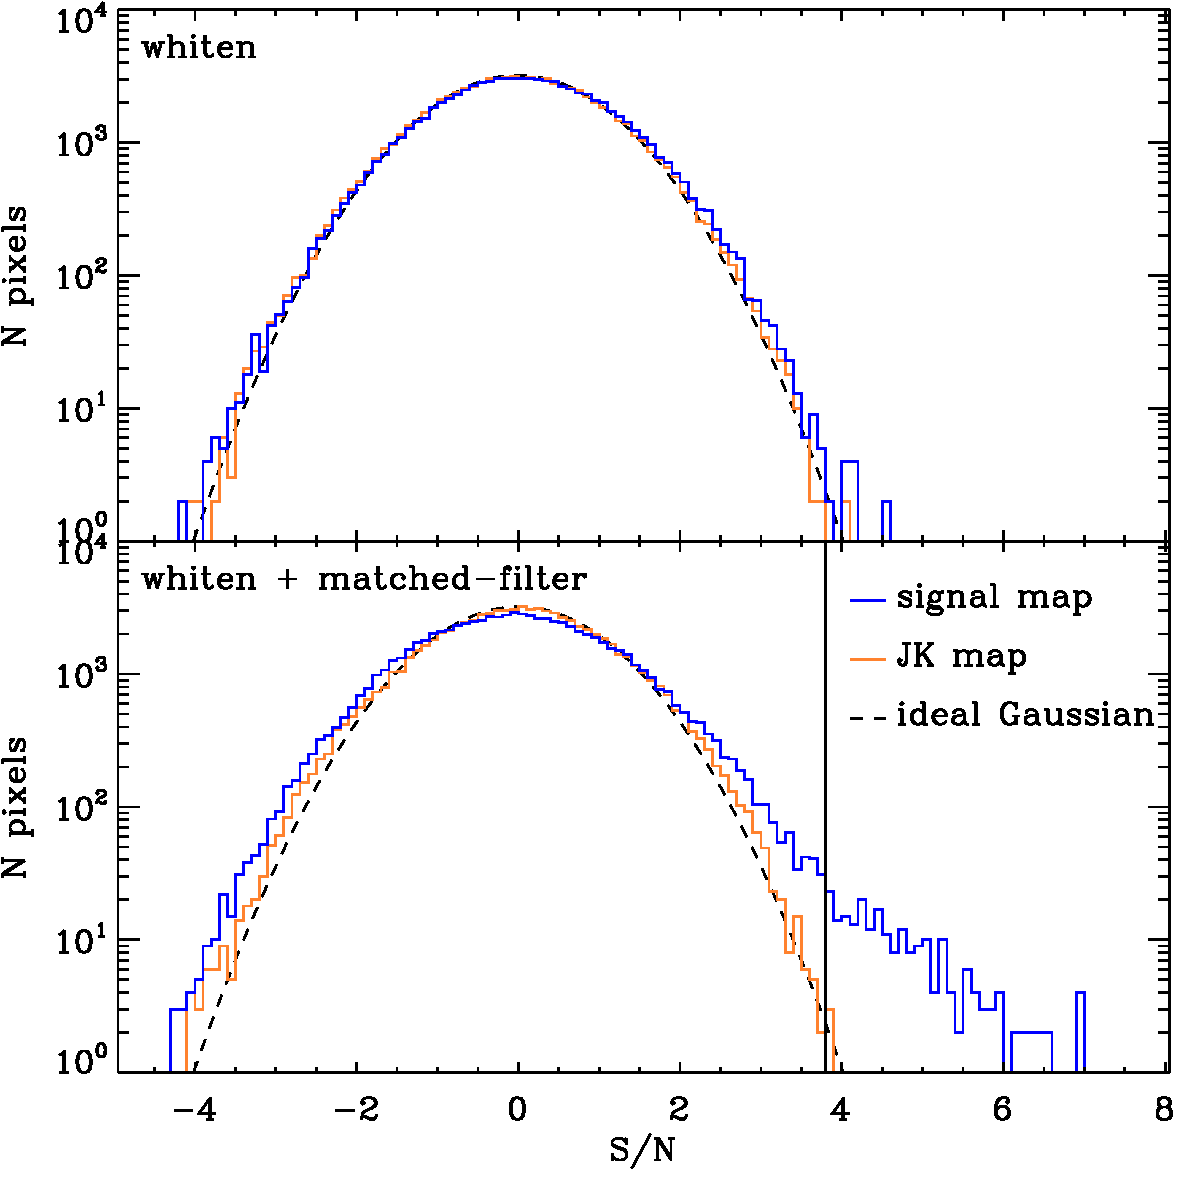
\includegraphics[width=\linewidth]{lockman_hist.pdf}
\caption{Histograms of S/N using pixels from the central region of
  Lockman Hole (second contour) in Fig.~\ref{fig:lockman_maps}a. The
  top panel shows the histograms for pixels from the whitened signal
  and jackknife maps (Figs.~\ref{fig:lockman_maps}b,e), compared to a
  Gaussian distribution with mean zero, standard deviation one, and an
  area normalized to the total number of pixels -- the expected
  distribution for a map of spatially-uncorrelated Gaussian noise. The
  good agreement indicates that these maps are indeed dominated by
  white noise, whose amplitude has been accurately estimated during
  map-making. The lower panel shows the results for matched-filtered
  signal and jackknife maps (Figs.~\ref{fig:lockman_maps}c,f). The
  filtered jackknife map distribution is still close to the
  expectation (Gaussian), but now the matched-filter has picked out
  significant signal leading to the large positive tail. The vertical
  solid line shows the chosen 3.8-$\sigma$ source-detection
  threshold.}
\label{fig:lockman_hist}
\end{figure}

As an additional external check, we have over-plotted orange ``$+$''
signs at the locations of 1.4\,GHz radio sources from \citet{owen2008}
with $S\gsim15$\,$\mu$Jy. Such radio catalogues have historically
proven invaluable for the precise identifications of high-redshift
submillimetre galaxies due to their relatively low surface densities
(compare with optical catalogues, for example), and a strong
correlation between the radio and submillimetre emission mechanisms
\citep[e.g.][]{smail2000,pope2006,ivison2007,chapin2009b}. Taking a
representative search radius of 8\,arcsec from these studies with
similar SNR sources and source sizes (the same size as the blue
circles), 9 out of 10 peaks in the smoothed signal map have potential
radio counterparts, whereas the single peak in the smoothed jackknife
map does not lie near any radio source. Again, a proper
cross-identification analysis must inevitably include simulations to
establish completeness, false-positive rates, as well as the effects
of point source clustering and confusion. See the aforementioned
papers and references therein for examples.

\begin{figure*}
\centering
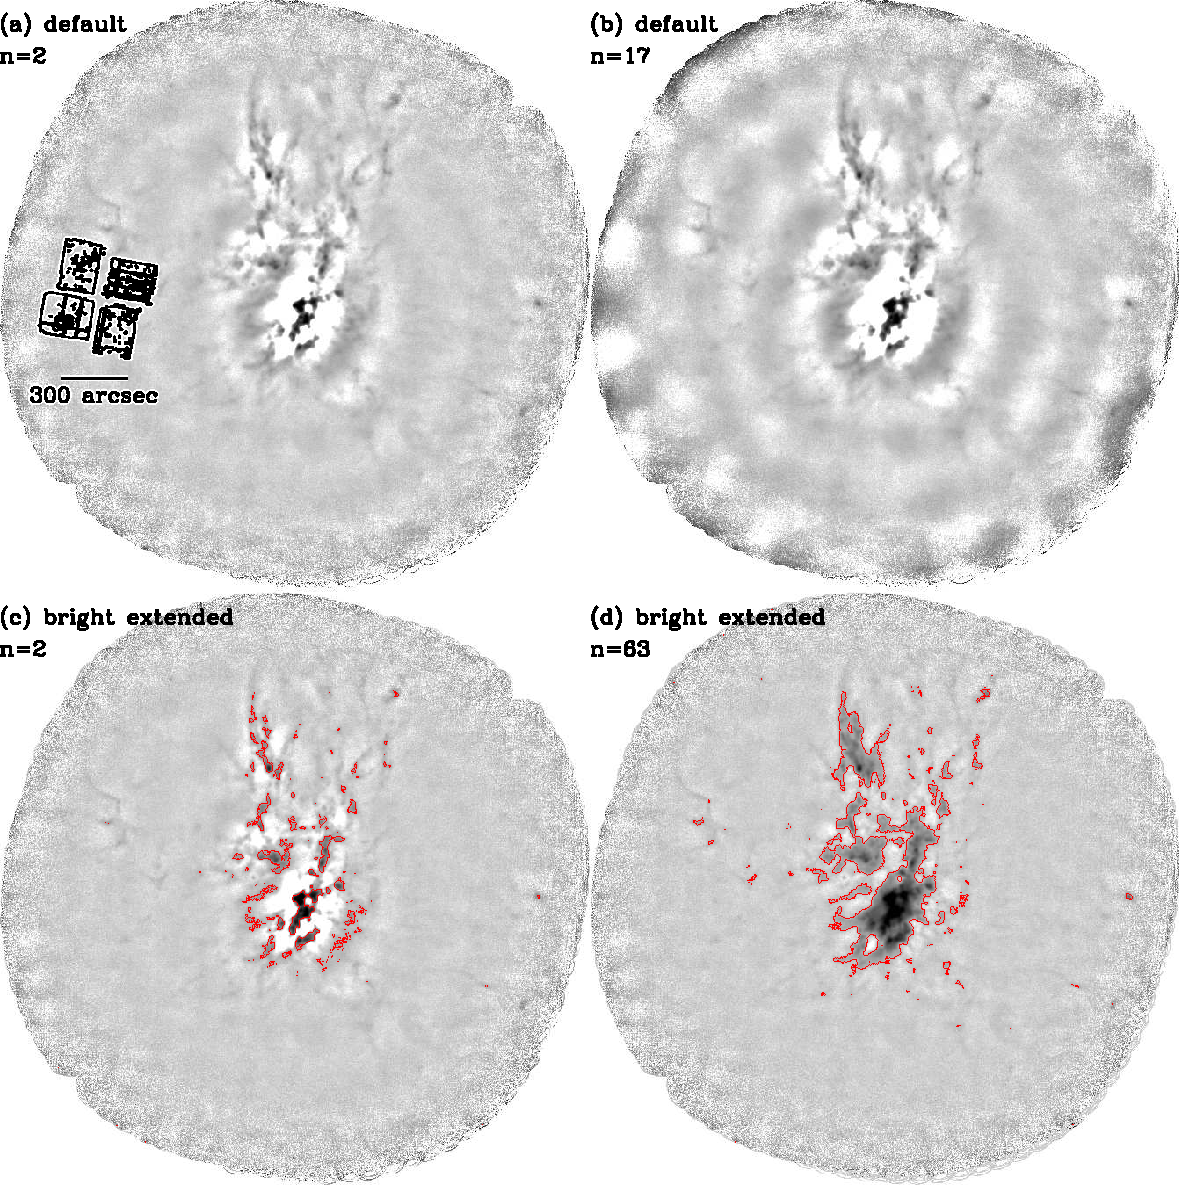
\includegraphics[width=\linewidth]{m17.pdf}
\caption{An 850\,\micron\ rotating pong map of M17. Intensity is
logarithmically scaled between -0.0003\,pw (white) and +0.01\,pW
(black). Iteration numbers are given in the corner of each
panel. Panels (a) and (b) show the results for a reduction using the
default parameters (the solution halted after reaching the default
map-based convergence criterion in 30 iterations). Panel (a) also
depicts the array footprint (position angle indicative of the start of
the observation), and a 300\,arcsec line shows the spatial scale
corresponding to the default \model{FLT} high-pass filter. Similar to
Fig.~\ref{fig:pointmaps}c, the lack of prior constraints on the map
leads to degeneracies, and therefore ripples on scales larger than the
array footprint (due to common-mode subtraction) and filter scale
(especially evident around the brightest peak at the centre of the
map). Panels (c) and (d) show the ``bright extended'' reduction, in
which a zero-mask is created iteratively from all of the pixels that
exceed a SNR of 5. While this region (red contour) only encompasses
the brightest peaks early in the solution, the final iteration it
identifies most of the bright, extended emission, and it significantly
helps with negative ringing.}
\label{fig:m17}
\end{figure*}

For future, significantly deeper \scuba\ maps, in which the RMS in a
PSF-smoothed map is dominated by point-source confusion, rather than
instrumental noise, a modified matched-filter will offer improved
results. See Appendix~A in \citet{chapin2011}, which shows how to
include confusion (when known \emph{a priori}) explicitly as a noise
term in the calculation of such filters.

%-------------------------------------------------
\subsection{Bright extended emission}
\label{sec:extended}
%-------------------------------------------------

In this final example, we analyze a map of M17 which contains bright,
extended emission, in contrast with the earlier two examples. A
promise of \scuba\ is to recover larger angular scales than what was
possible with earlier-generation ground-based submillimetre
cameras. The two main factors contributing to this expectation are:
(i) a larger array footprint on the sky which should make the
subtraction of common sky-emission signals more effective; and (ii)
fast detectors (with a correspondingly fast sample rate) to enable
higher slew-rates (up to 600\,arcsec\,s$^{-1}$) to capture as much
large-scale structure as possible above the detector $1/f$ knees. We
produce maps of observation 11 on 20110531 using the 850\,\micron\
array. It is a rotating PONG covering a diameter of 0.375\,deg, with a
scan speed of 300\,arcsec\,s$^{-1}$, and a transverse spacing of
180\,arcsec, taking 37.5\,min to complete.

The default reduction of these data is shown in the top panels of
Fig.~\ref{fig:m17}, after iterations 2 (the first map estimated after
the noise weights have been measured) and 17 iterations (when the map
has converged). The first panel also depicts the array footprint, and
the angular scale corresponding to the high-pass filter edge. Much
like the reduction of a point source without any prior constraints
(Fig.~\ref{fig:pointmaps}c), degeneracies on scales larger than the
array footprint and filter produce ripples in the map.

Unlike the case of a known point-source (Section~\ref{sec:point}), it
may not be possible for the observer to define, in advance, a mask of
regions containing blank sky. Indeed, for this map, much of the field
clearly contains extended structures. Furthermore, the goal of such
maps may be to detect \emph{previously unknown} cool, dense regions of
the ISM that may not have appeared at other wavelengths (e.g. the
first optically-thick cloud-collapse stages of star-formation). While
the option does exist for the user to supply their own mask, a
facility has been added to SMURF to generate one automatically by
flagging pixels above some SNR threshold after each iteration as part
of the ``bright extended'' configuration.

The results of this automatic masking are shown in the bottom panels
of Fig.~\ref{fig:m17}. After the second iteration, only narrow regions
around the brightest peaks are identified. However, as the solution
progresses, the negative bowls around the bright sources are slowly
reduced and the mask ``grows'' out from the brightest areas. By the
final iteration, most of the obvious structures in the data are
encompassed by the mask, negative bowling is significantly reduced,
and the brightest regions are clearly more extended.


\begin{figure*}
\centering
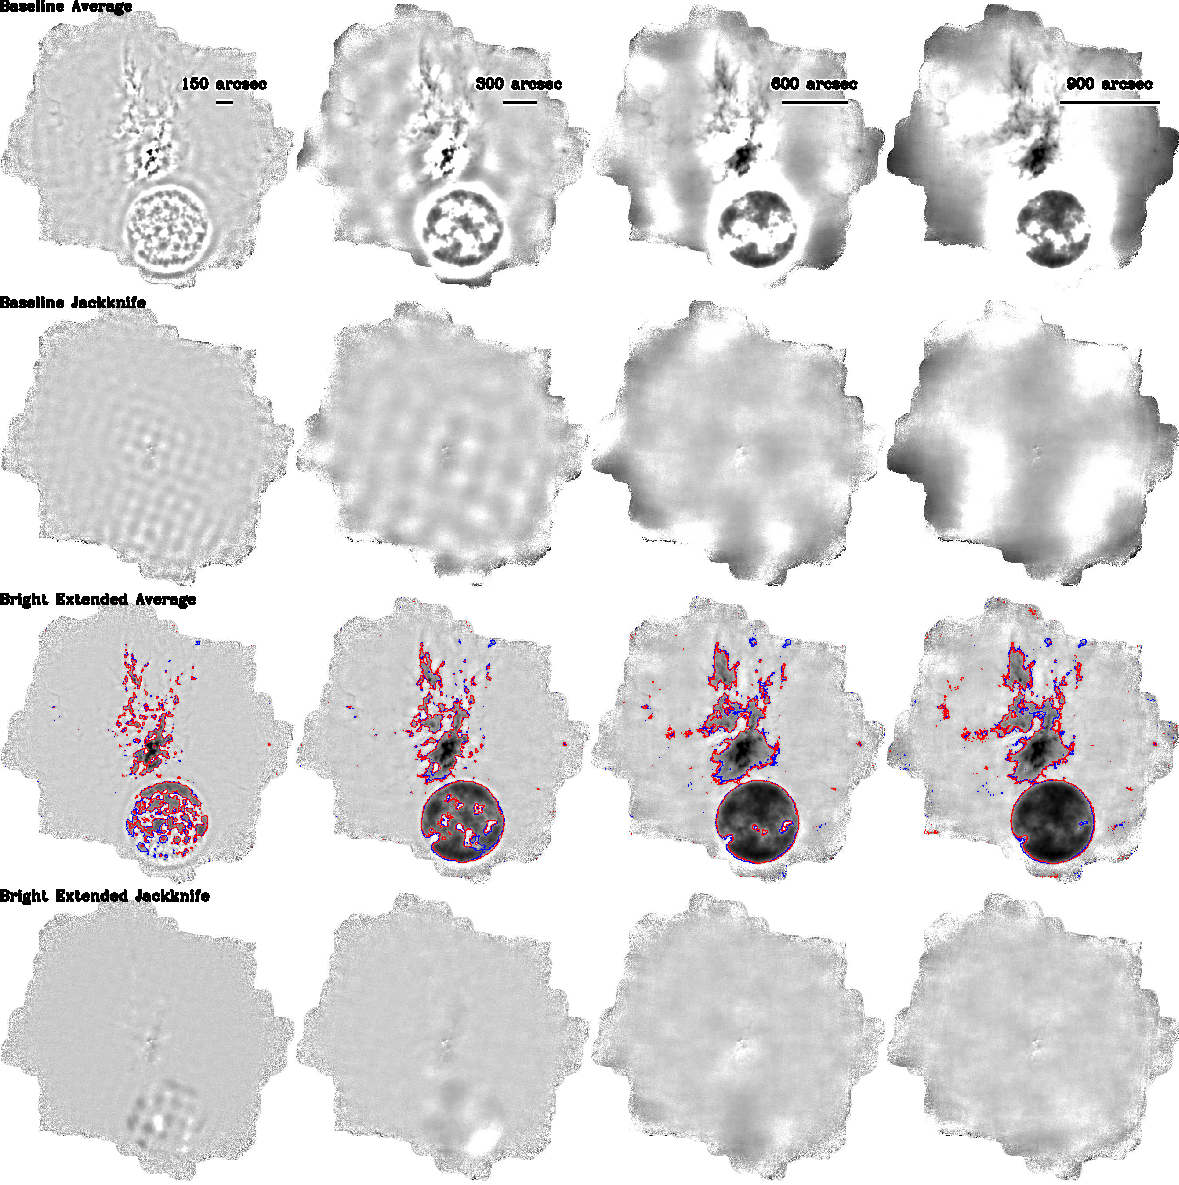
\includegraphics[width=\linewidth]{m17_jk.pdf}
\caption{Maps of M17 used to characterize the noise properties and
transfer function of SMURF (same intensity scale as
Fig.~\ref{fig:m17}). For each column, a different high-pass filter
edge scale was adopted (indicated in the top panels). First (top) row:
Average of two halves of the data analyzed independently, using the
default configuration. The data have had added to them synthetic
signal within a 600\,arcsec diameter circle (S.E. of M17) created as a
realization of noise from a $P(k) \propto k^{-3}$ angular power
spectrum multiplied by the PSF, subtracting the minimum to make it
positive, scaling it to a similar signal range as M17 itself, and
rolling-off the edges smoothly using half a period of a radial
(1+cosine)/2 function across 100\,arcsec beyond the edge of the
600\,arcsec region. Second row: jackknife maps produced from the
differences of the maps of each half of the data that went into the
first row. Third row: average of the two halves of the data using the
bright extended reduction. The blue and red contours indicated the
zero-masked regions in each case (note for the 300\,arcsec case that
the region about M17 matches fairly closely the mask in
Fig.~\ref{fig:m17}d). Clearly as the filter scale is increased, due to
the high SNR of the data, larger emissions regions are (correctly)
detected and reproduced in the map. Fourth (bottom) row: Jackknife
maps for the bright extended reductions.}
\label{fig:m17_jk}
\end{figure*}

\begin{figure*}
\centering
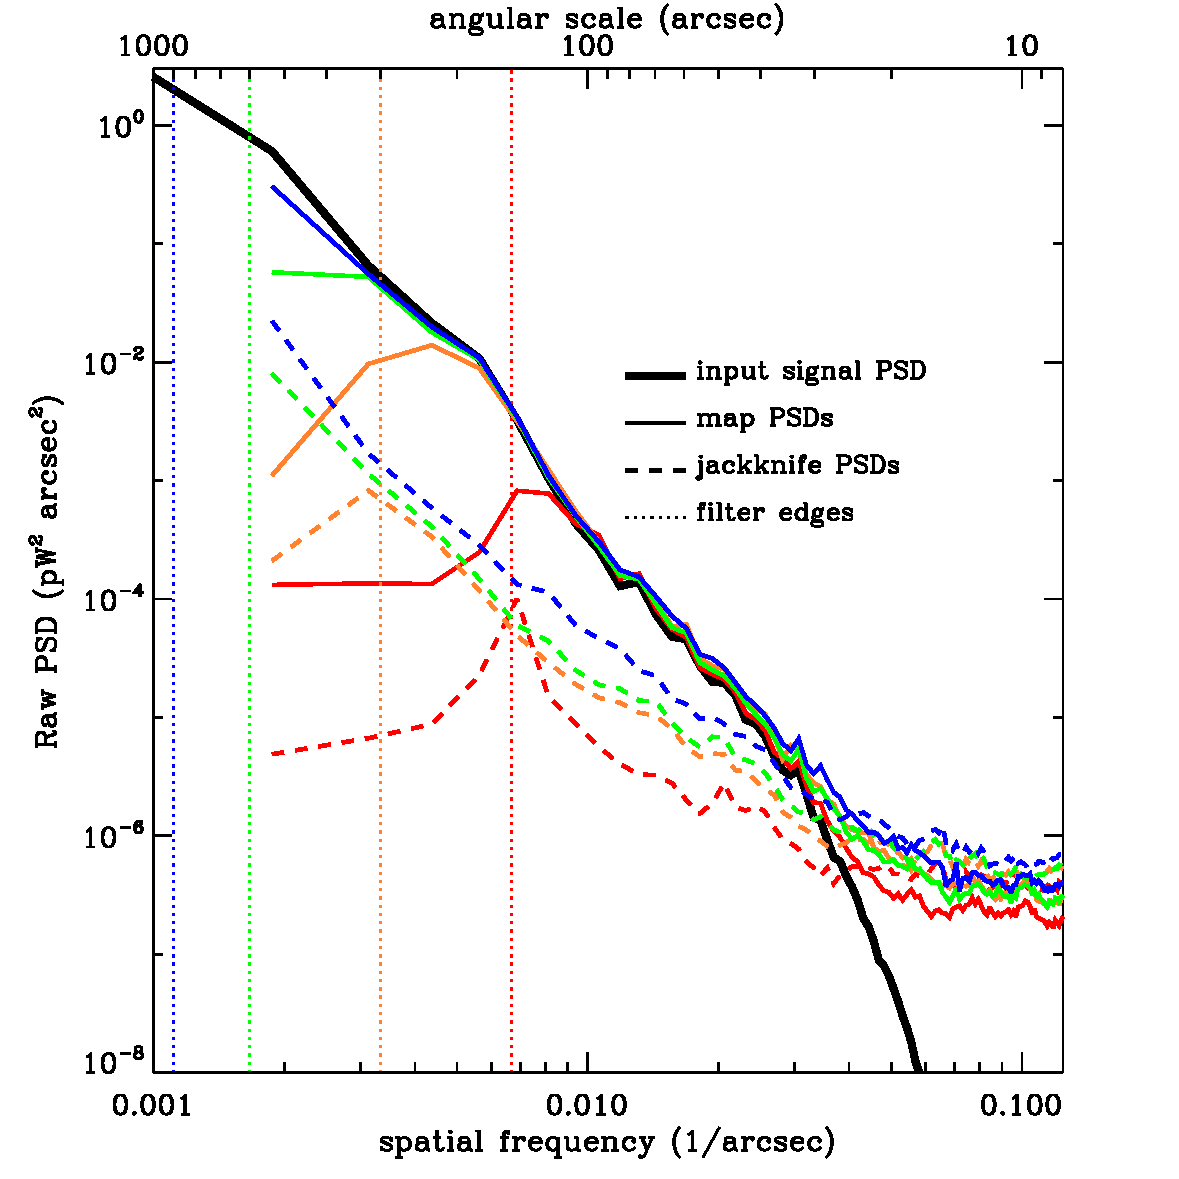
\includegraphics[width=0.49\linewidth]{pspec_m17_default.pdf}
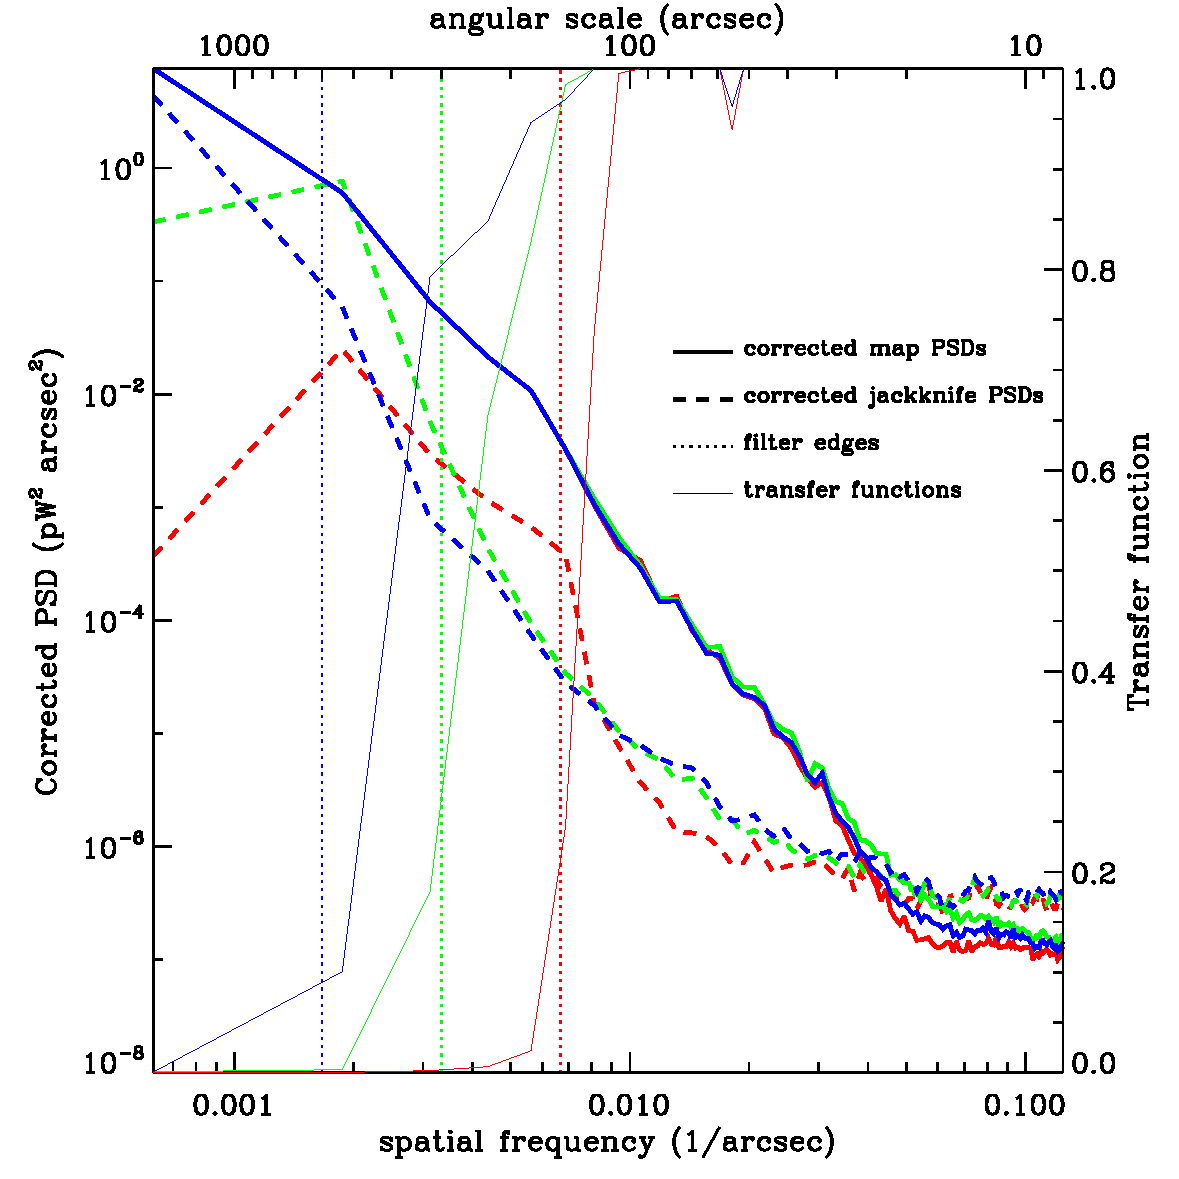
\includegraphics[width=0.49\linewidth]{cor_pspec_m17_default.pdf}
\caption{Angular power spectral densities (PSDs) for the region of the
M17 map in Fig.~\ref{fig:m17_jk} containing synthetic data, using the
default configuration. left: raw PSDs for the input (noiseless)
simulated data (thick black line), the signal (average of each half)
PSDs (thin solid lines), and noise PSDs estimated from the jackknives
(dashed lines). Vertical dotted lines indicate the high-pass filter
scales: 150\,arcsec (red); 300\,arcsec (orange); 600\,arcsec (green);
and 900\,arcsec (blue). Since the input PSD is known, it is possible
to measure the transfer function of the map-maker as the ratio between
the output map signal PSDs and the input PSD (from the left panel),
giving the thin coloured lines (linear vertical axis shown on right of
plot). The remaining lines are as in the left panel, but now corrected
by the transfer function. This plot shows that increasing the filter
scale improves the SNR at intermediates scales
($\sim$200--600\,arcsec), although the SNR worsens at smaller scales
($\lsim$200\,arcsec).}
\label{fig:m17_def_ps}
\end{figure*}

\begin{figure*}
\centering
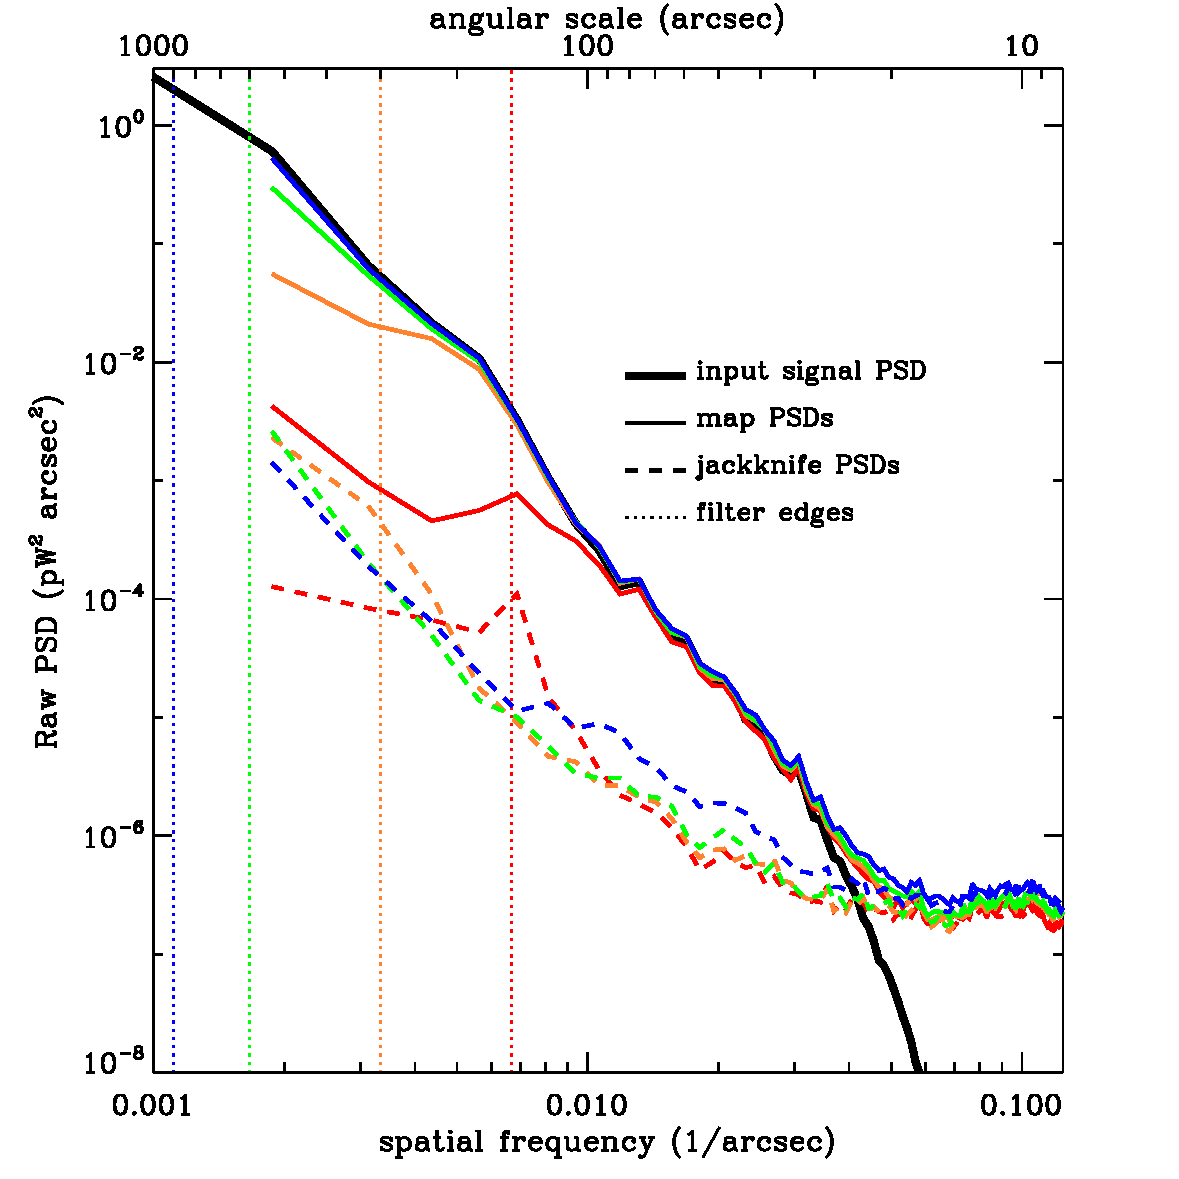
\includegraphics[width=0.49\linewidth]{pspec_m17_bright_extended.pdf}
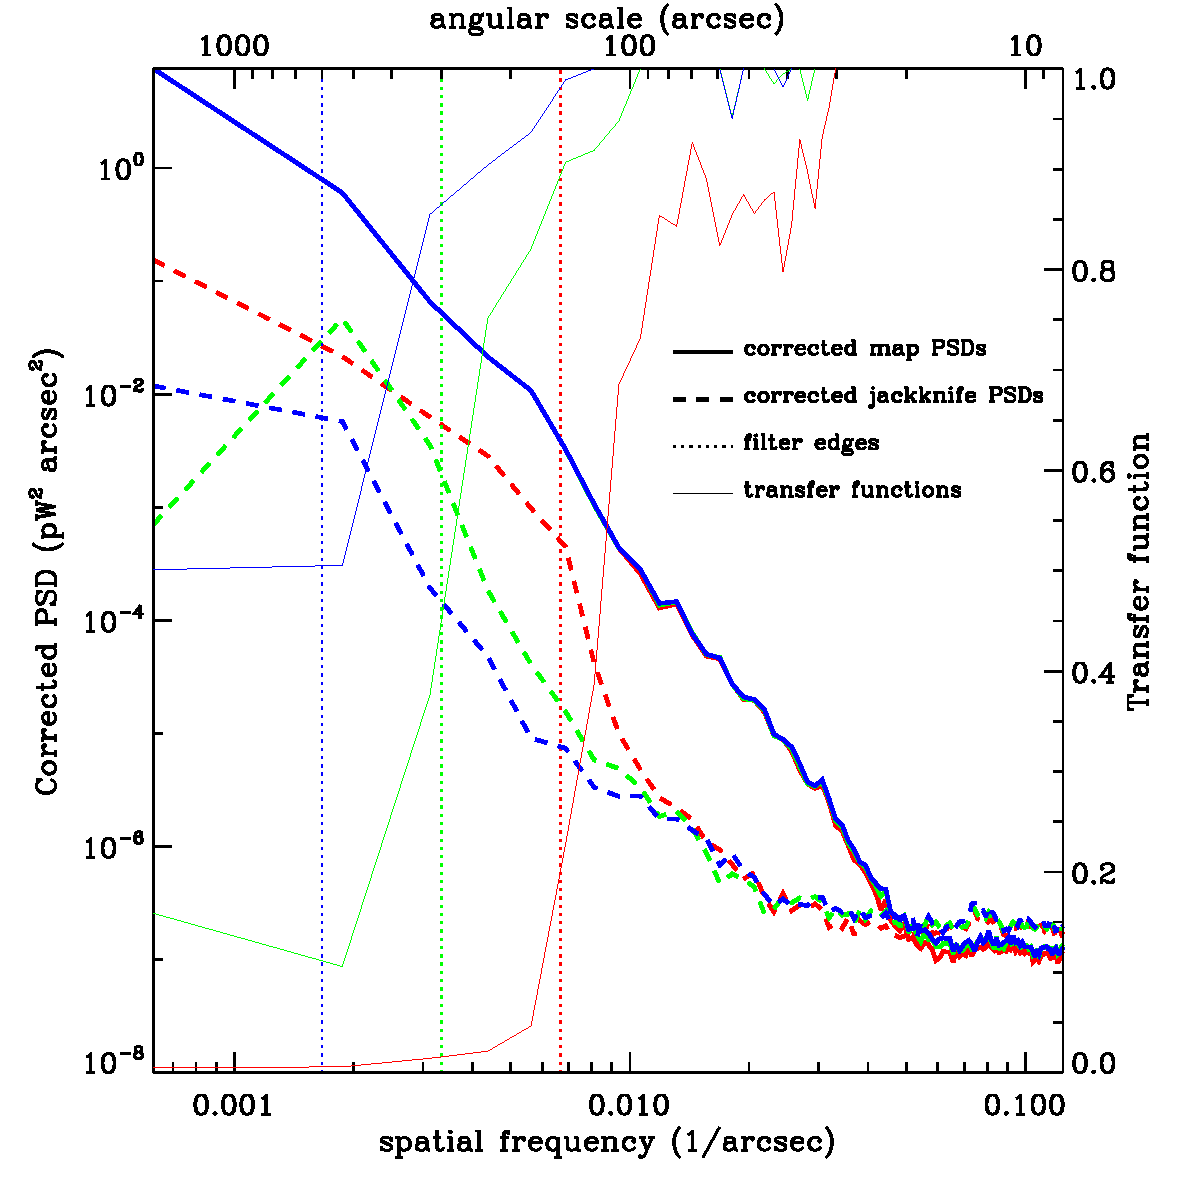
\includegraphics[width=0.49\linewidth]{cor_pspec_m17_bright_extended.pdf}
\caption{Lines have same meaning as in Fig.~\ref{fig:m17_def_ps},
except now using the bright extended configuration. This configuration
has resulted in an improved transfer function and SNR at large angular
scales. Also note that increasing the filter scale does not have as
large of an impact on the small-scale noise as in the default
configuration, although it is still noticeably larger up to scales of
about $\sim$60\,arcsec.}
\label{fig:m17_be_ps}
\end{figure*}

While the reduction in the bottom panels of Fig.~\ref{fig:m17} is
clearly superior in at least a cosmetic sense to those in the top
panels, it is important to quantify both the noise properties of the
maps and their response to real structures (the transfer function). We
would also like to know how each are affected by our choice of filter
scale.  Similar to the previous section, we will use a jackknife test
to estimate the noise, as well as injecting known sources into the
data to observe how they are attenuated.

Maps are produced using the first and second continuous halves of the
data in Fig.~\ref{fig:m17_jk}. This is not an ideal situation since
the noise properties may evolve with time (e.g., due to changing sky
conditions) leading to a biased estimate of the parent noise
distribution in the complete map from the jackknife. Also, since the
zero-masking depends on the SNR of the map, it will be restricted to
regions approximately $\sqrt{2}$ shallower in these maps than for the
full data set. Finally, the cross-linking (positional angles sampled)
is similar, though not identical in the two halves. Ideally one would
have many full maps as in the case of the Lockman Hole data in the
previous section, from which alternating maps could be combined.

Since our goal in this section is to measure the response of the
map-maker to extended structures, we inject a simulated signal with
power at a range of scales to a relatively empty region of the map.
It is created by drawing a realization of noise within an 800\,arcsec
on-a-side box, with an angular power spectrum $P(k) \propto k^{-3}$
which is appropriate for Galactic cirrus clouds
\citep[e.g.][]{gautier1992}. It is then filtered again with a
14.5\,arcsec Gaussian to model the effect of the \scuba\ optical
response. The RMS of these fluctuations are then normalized to 0.002
pW so that they are comparable to the dynamic range of M17 itself. The
minimum is subtracted so that the signal is positive. Finally, half a
period of a (1+cosine)/2 function is used to roll-off the signal to
zero between radii of 300 and 400 arcsec.

The first row of Fig.~\ref{fig:m17_jk} shows the total signal image
averaging the maps made of each independent half of the data, for the
default configuration (inverse-variance weighting has been used). The
columns show reductions using 150, 300, 600, and 900\,arcsec filter
edges in the reductions. For reference, the largest scale that is
completely inscribed by the array footprint is about 400\,arcsec, and
the diagonal of the array is about 600\,arcsec (meaning that scales
beyond 600\,arcsec are completely unconstrained when common-mode
rejection is used).  The synthetic data are clearly seen as the
circular region S.E. of M17. As the filter scale is increased, the
size of the ripples increases accordingly. While larger structures do
seem to appear, negative bowls are a major problem without any other
map constraints.The second row of Fig.~\ref{fig:m17_jk} shows the
jackknife maps. The astronomical emission is almost perfectly removed,
except for a slight impression of M17 near the centre of the map that
is probably due to some combination of detector gain and pointing
drifts. Otherwise the jackknife appears to be a plausible realization
of noise from the same parent distribution as for the averaged maps.

The third and fourth rows in Fig.~\ref{fig:m17_jk} repeat this
exercise using the bright extended configuration, in which the SNR
threshold of 5 is again used to constrain the map. As the filter scale
is increased, more of the extended structure in M17 is reproduced in
the map, as evidenced by the blue and red contours (masks generated
from the first and second halves of the data, respectively). The
masking does a generally good job of suppressing the largest-scale
ripples that are produced by the default reduction. However, the noise
away from regions of bright emission does increase noticeably (mottled
appearance). With filter scales $\gsim600$\,arcsec, virtually the
entire region of synthetic emission is correctly identified by the SNR
mask and allowed to vary freely in the solution.

Next, we analyze the angular power spectra densities (PSDs) of the
maps to understand the signal and noise properties of the map-maker in
the region of synthetic sources, as a function of filter scale. The
left panel of Fig.~\ref{fig:m17_def_ps} shows the raw PSDs for the
input synthetic signal (thick black line), the output map signals
(thin solid lines), and the jackknife maps (dashed lines). Colours
encode the filter scales used: 150\,arcsec (red); 300\,arcsec
(orange); 600\,arcsec (green); and 900\,arcsec (blue). Note that, in
the exception of the synthetic data, we only plot the PSDs down two
the second-lowest spatial frequency bin of
$1.875\times10^{-3}$\,arcsec$^{-1}$, or 533\,arcsec, due to the fact
that the smallest is very poorly sampled, and therefore noisy. As the
filter edge is increased, more power is measured in the map PSDs at
larger scales. However, much of this power is clearly produced by
noise which appears in the jackknife PSDs. We estimate the map-maker
transfer function as the ratio between the portion of the signal PSDs
\emph{not} produced by noise, to the input PSD, or
%
\begin{equation}
G(k) = \frac{P_\mathrm{M}(k) - P_\mathrm{JK}(k)}{P_\mathrm{S}(k)},
\end{equation}
%
where $k$ is the spatial frequency, and the subscripts ``M'', ``JK'',
and ``S'' refer to the signal map, jackknife map, and synthetic map,
respectively.

The transfer functions $G(k)$ are plotted as thin solid lines in the
right panel of Fig.~\ref{fig:m17_def_ps}. This formula produced
extremely noisy values at large frequencies (small scales), and was
set to a value of 1 above 0.015\,arcsec$^{-1}$, as well as any point
in the curve where $P_\mathrm{M}(k)$ exceeded $P_\mathrm{S}(k)$
(i.e. $G(K)$ is assumed to be $\le$1). As expected, the larger the
scale of the filter, the lower the spatial frequency at which the map
transfer function falls. We then correct the map and jackknife PSDs by
dividing by $G(k)$ to produce the thick solid, and dashed lines in the
right panel of Fig.~\ref{fig:m17_def_ps}. This shows us that, even
though the raw noise in the left panel is lower at small scales when a
smaller-scale filter is used (e.g. the red dashed line), once we
correct for the transfer function, we actually win in a SNR sense at
large scales using the larger-scale filter as you would expect.

These tests are then repeated using the bright extended reduction in
Fig.~\ref{fig:m17_be_ps}. The most obvious improvement with this
reduction over the default reduction is that the transfer functions
fall more slowly at large angular scales, accompanied by a slower
increase in noise; in other words, there is greatly improved SNR at
large angular scales (an obvious conclusion given the appearence of
the maps in Fig.~\ref{fig:m17_jk}). In fact, using the 900\,arcsec
filter edge, the map response is still above 80\% right out to the
largest scale accurately measured in the PSDs, 533\,arcsec, which is
about the largest scale that should be recoverable given the size of
the array footprint and the fact that we use common-mode rejection.
Another interesting feature of these reductions is that the increase
in small-scale noise as the filter edge is increased is not as drastic
as in the default reduction, and the SNR improves at scales
$\gsim$60\,arcsec.

One case in which the SNR is \emph{worse} using the bright extended
reduction is using a 150\,arcsec filter. In this case the noise is
considerably larger in the bright extended reduction as evidenced by
the ``kink'' near 150\,arcsec. Referring to the mask contours in the
left panel of the third row, it is clear that the map-maker has failed
to identify much of the bright, extended emission in the region of the
synthetic source. Each area that is not within the contours is
constrained to zero throughout the solution, therefore suppressing
power (and lowering the transfer function), and subsequently reducing
the SNR of the final result. This measurement serves as a warning: the
map-maker response is non-linear when using SNR masking. Harsh
filtering can provide misleading results as in this example. Maps of
\emph{faint} extended emission will also suffer considerably, as the
structures of interest may not clear the SNR threshold for the mask.

Note that alternatives to the zero-masking approach do exist for other
iterative map-makers. For example, \citet{kovacs2008} typically
restricts the solution to a small fixed number of iterations (of order
$\sim$10), although we note that there is no guarantee that maps will
have reasonably converged with such a strategy. For BOLOCAM data of
the Galactic Plane, \citet{aguirre2010} used a Maximum-Entropy
filtering step to suppress large-scales. As in the case of the
SNR-based masking described here, Maximum-Entropy filtering is also
non-linear, meaning that it too requires simulations to establish its
transfer function and noise properties as a function of angular scale.


%------------------------------------------------------------------------------
\section{Summary and future work}
\label{sec:summary}
%------------------------------------------------------------------------------

\begin{enumerate}

\item SMURF is an iterative map-maker that can produce \scuba\ maps on
single high-end modern desktops in a reasonable amount of time.

\item A simple model which removes most noise in a common-mode
rejection step, along with high-pass filtering, results in maps that
approach the white-noise performance of the detectors.

\item The main problem to overcome with our strategy is the divergence
of the map on large angular scales, due to the degeneracy between the
map, common-mode, and other residual low-frequency noise. A simple
strategy of constraining empty regions of the map to zero (either a
user-supplied mask for known sources, or an iterative determination of
signal above some SNR threshold) provides good constraints for compact
objects, and bright/extended structures.

\item For maps of faint point sources, a single (non-iterative)
high-pass filter at the start of the reduction produces maps that are
nearly white-noise limited. We illustatre how to completely whiten the
maps using jackknife measurements of the angular noise power spectrum
in order to reliably extract sources down to the limits of the map.

\item The map-maker has an automatic stopping criterion based on the
change in the map and $\chi^2$ between subsequent iterations, allowing
it to adapt to a wide range of data in a pipeline setting.

\item It is believed that a maximum-likelihood map-maker, such as
SANEPIC, will provide improved maps over the iterative algorithm
described here. However, SMURF will most likely be used as an initial
step in such processing since it can quickly clean the bolometer
time-series, as well as perform map-based despiking (a necessarily
iterative step).


\end{enumerate}

%\scuba\ is being re-commissioned. Maybe we will have some initial data
%on fridge performance? If both it, and sky noise are relatively
%well-behaved, might be able to restrict filtering to lower frequencies
%and get larger-scale structures.

%Larger array footprint also helps.

%Talk about potential of Pascale et al. method to get closer to
%max-likelihood map solution (handle maps at constant scan angles with
%weights in Fourier space separately).

%------------------------------------------------------------------------------
\section{Acknowledgements}
%------------------------------------------------------------------------------

\textit{Presumably the standard telescope acknowledgment here plus a
thank you to CFI for funding the DR work. Ed should probably thank
both CANFAR and JAC for additionally funding although his JAC funding
is noted in the affiliation.}

%------------------------------------------------------------------------------
\bibliographystyle{mn2e}
\bibliography{mn-jour,refs}
%------------------------------------------------------------------------------

%------------------------------------------------------------------------------
\appendix
\section[]{Step correction in detail}

An outline of the step correction algorithm is given in
Section~\ref{sec:steps}. This appendix contains a more detailed
description.

Detecting and correcting steps in a single bolometer time stream involves:

\begin{enumerate}

\item Locating each candidate step.

\item Determining the widths of the candidate steps.

\item Determine the height of the step. Steps can vary enormously in height.
For instance the step in the left plot of Fig.~\ref{fig:steps1} is
roughly 3 pW in height, whereas the step at sample 5100 in the right hand
plot is only 0.01 pW in height. The height of a step is taken as the
difference in the local median value just before and just after the step.

\item Correcting all subsequent data values by the step height.

\item Once all steps have been corrected, a global offset is added to the
corrected bolometer time stream to ensure that the mean value before and
after step correction is unchanged.

\end{enumerate}

\subsection{Detecting candidate steps}
The first stage in the algorithm is to search the bolometer time stream for
contiguous blocks of samples that have unusually large mean gradients
compared to the neighbouring samples. Each such block of samples is
considered to be a candidate step. The starting and ending time of each
such block is noted. Once all candidate steps have been found for a
bolometer, the algorithm proceeds to the next stage. Candidate steps are
found as follows:

\begin{enumerate}

\item Smooth the bolometer time stream using a median filter of width
50 samples. This reduces the effects of the noise in the data. Using a
median filter rather than a mean filter helps to preserve the sharp edges
at each step, and is robust against spikes, etc.

\begin{figure}
\centering
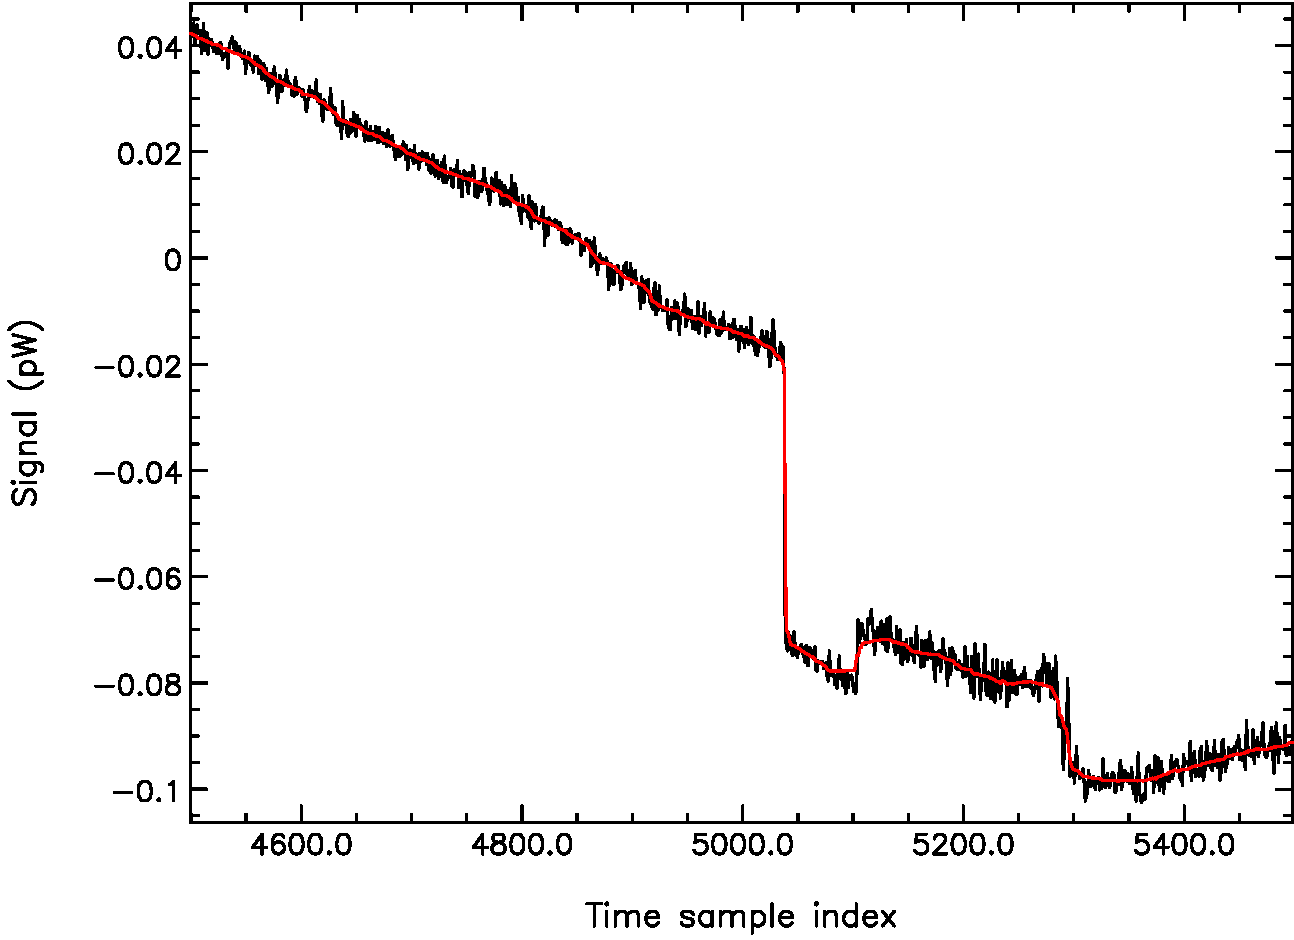
\includegraphics[width=\linewidth]{steps2.pdf}
\caption{A section of the right hand bolometer from  Fig.~\ref{fig:steps1}
with the median smoothed data overlayed in red.}
\label{fig:steps2}
\end{figure}

The red curve in Fig.~\ref{fig:steps2} shows the median smoothed data for
the right hand bolometer from Fig.~\ref{fig:steps1}.

\item At each time sample, find the difference between the two adjacent
values in the median filtered bolometer data. This is proportional to the
gradient of the median filtered bolometer data. Fig.~\ref{fig:steps3}
shows these differences for the sample bolometer shown in previous
figures. The high gradients at the three step are clearly visible at
indices 5040, 5100 and 5280.

\begin{figure}
\centering
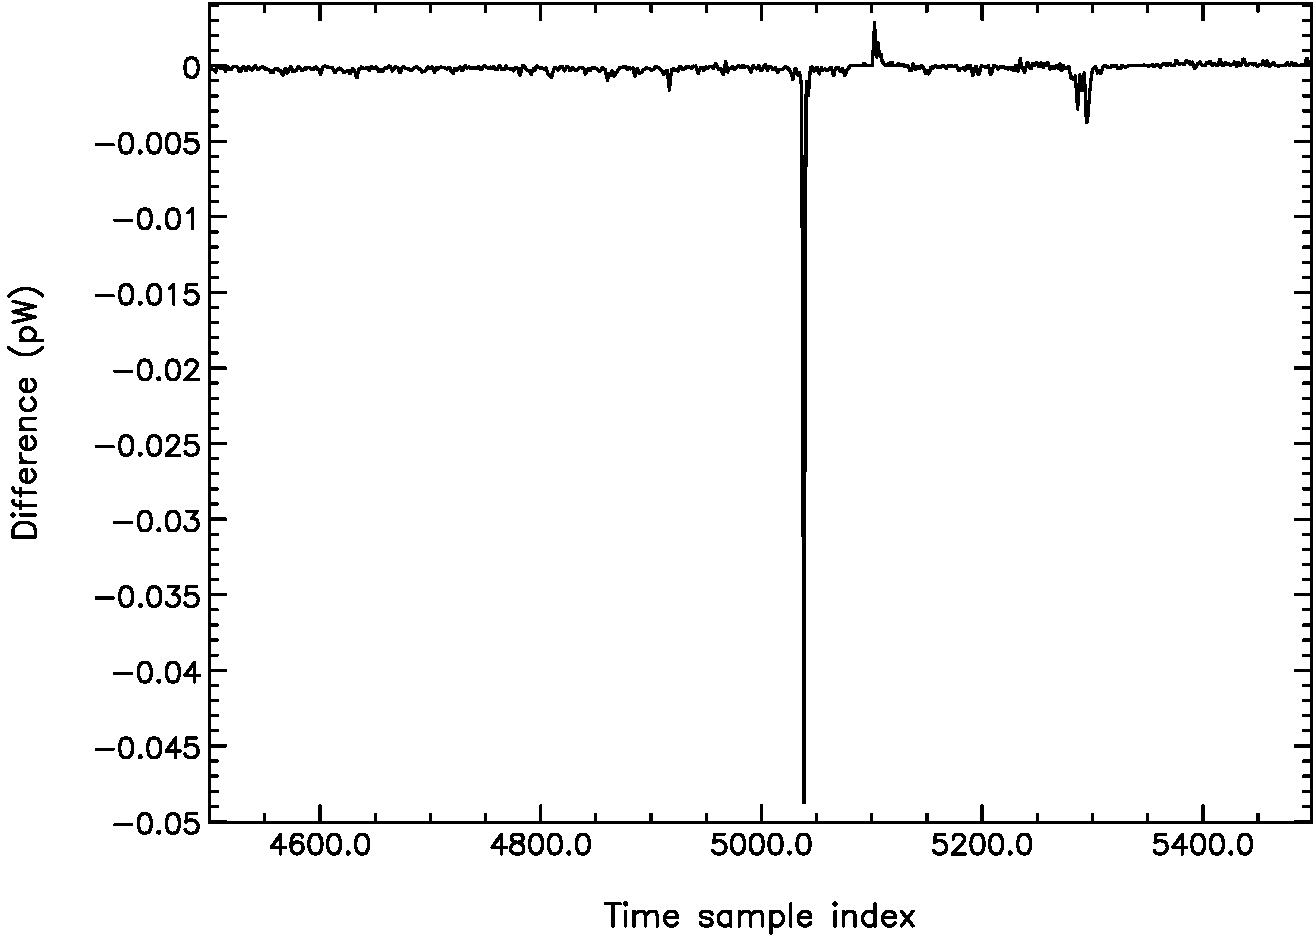
\includegraphics[width=\linewidth]{steps3.pdf}
\caption{Differences between adjacent values of the median smoothed data
in  Fig.~\ref{fig:steps2}.}
\label{fig:steps3}
\end{figure}

\item Steps are located by looking for difference values that exceed 25
times the RMS value of the nearby neighbouring differences. However, the
local RMS of the differences includes the gradient of the underlying
noise-free time series. So if there is a strong upward or downward trend
in the time series data, the RMS of the difference values will be higher,
potentially resulting in some steps being missed. For instance, at sample
5000 the overall trend in the time series is downwards, resulting in a
negative bias to the difference values.\footnote{This bias is not visible in
Fig.~\ref{fig:steps3} because of the large vertical range, but can be seen in
Fig.~\ref{fig:steps4} which has a smaller vertical scale.}

Therefore to enhance the reliability of the step detection, such biases
are removed before locating the steps. To do this, the differences are
smoothed using a mean filter, and the smoothed differences are removed.
The remaining residual difference values represent the gradient due to
steps, spikes, noise, etc. It is important that the smoothed differences
are not polluted by the large values caused by spikes and steps. So
before smoothing, differences of more than three times the RMS difference
(taken over the whole time stream) are identified and flagged. The RMS is
then re-calculated omitting the flagged values and a further two such
rejection iterations are performed. This process flags high gradient values
caused by spikes, jumps, point sources, etc. The difference values close
to a step are often not typical of those in the wider neighbourhood, so
each block of contiguous flagged difference values is doubled in width.
These flagged values are shown as black in Fig.~\ref{fig:steps4}, with
the remaining unflagged values shown in red.

\begin{figure}
\centering
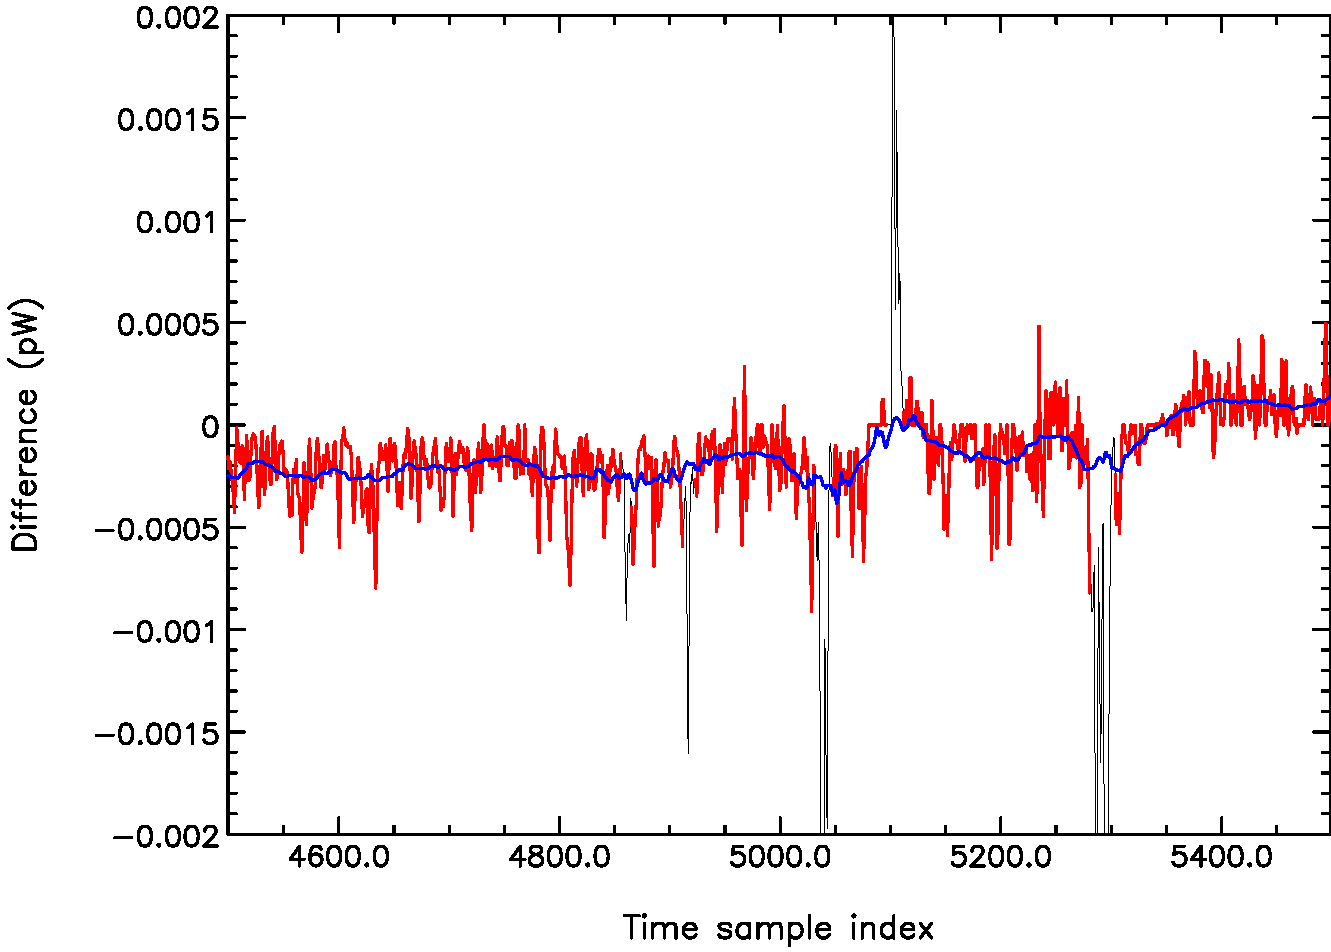
\includegraphics[width=\linewidth]{steps4.pdf}
\caption{The red curve shows the data from Fig.~\ref{fig:steps3} plotted with smaller upper
and lower limits. The blue curve shows the results of smoothing the red
curve. Points omitted from the red curve are shown in black.}
\label{fig:steps4}
\end{figure}

\item The differences for the remaining samples are smoothed
using a mean filter of width 50 samples. The smoothing process fills in small
holes in the array (up to 40 samples), but will not fill in larger holes.
Such larger holes are filled in later by linear interpolation. The
resulting smoothed differences (shown in blue in Fig.~\ref{fig:steps4})
provide an estimate of the local gradient of the underlying noise-free
median-filtered data stream.

\item The smoothed differences are subtracted from the total differences
to get the residual differences caused by noise, spikes, steps, etc.
These are show in black in Fig.~\ref{fig:steps5}.

\item The local RMS of the residual differences at each time sample is
found by smoothing the squared residual differences using a median filter
of width 200 samples, and then taking the square root of the smoothed values.
These are show in green in Fig.~\ref{fig:steps5}.

\begin{figure}
\centering
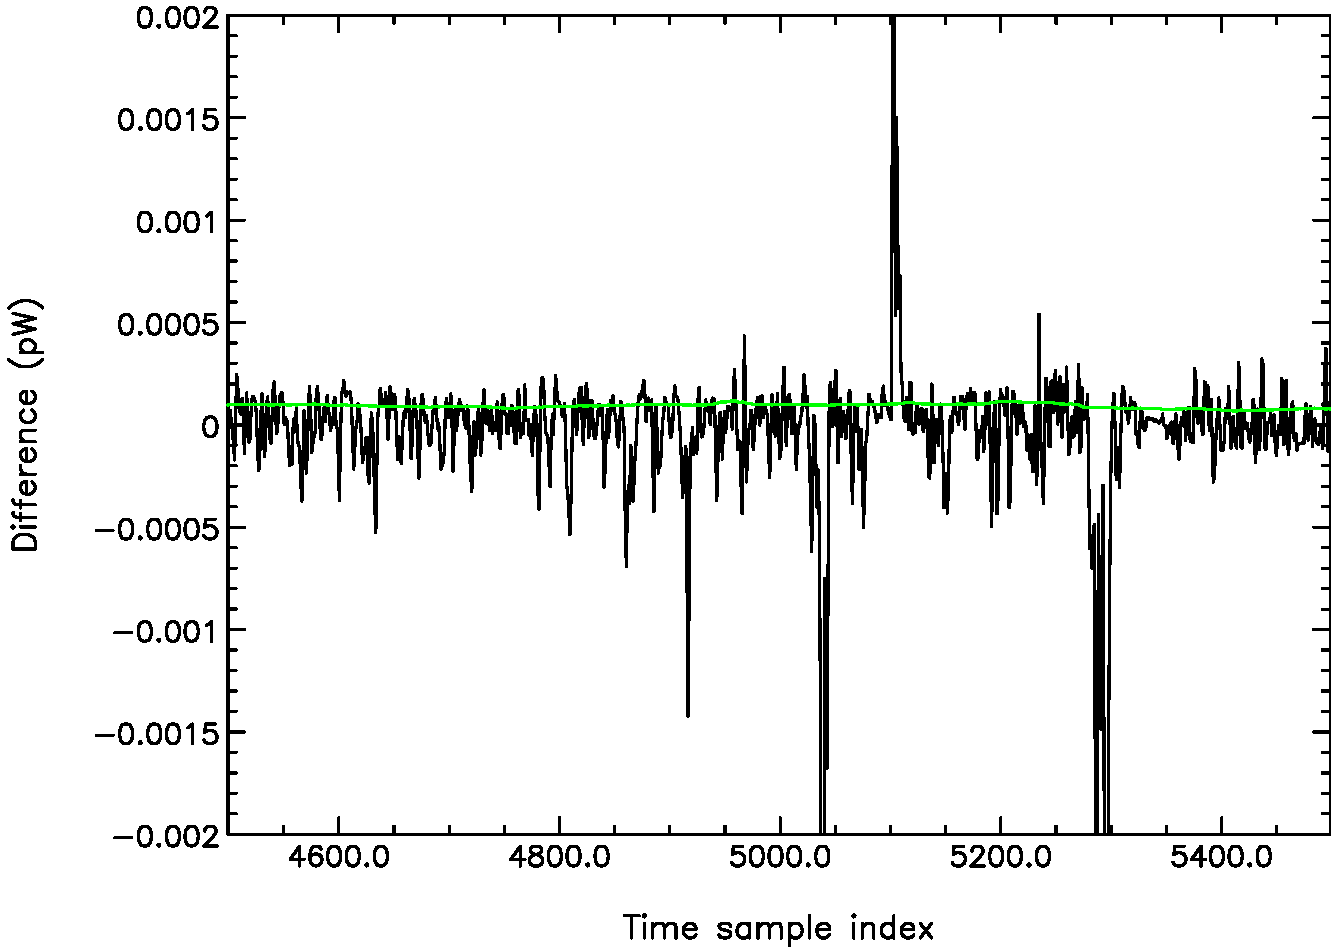
\includegraphics[width=\linewidth]{steps5.pdf}
\caption{The black curve shows the residuals between the red and blue curves in
Fig.~\ref{fig:steps4}. Missing data is filled in by a combination of
smoothing and linear interpolation. The green curve is the local RMS of the data
over a box width of 200 samples.}
\label{fig:steps5}
\end{figure}

\item Blocks of contiguous samples for which the residual difference exceeds
25 times the local RMS of the residual differences are found. Any two
such blocks that are separated by fewer than 100 samples are merged into
a single block. Blocks are ignored if they fail any of the following
tests:

\begin{enumerate}

\item The width of the block must be less than 200 samples.

\item The total of all the SNR values (the absolute residual difference
divided by the local RMS of the residual differences) in the block must be
at least 25.

\item The total of all SNR values in the block must exceed half the value of
the largest single SNR value in the block.

\end{enumerate}

The second and third tests are intended to prevent spikes being treated as
two very close steps, since such steps will have SNR values of opposite
signs and will thus cancel out.

The data in Fig.~\ref{fig:steps5} results in two blocks being defined -
one between samples 5037 and 5102 and another between samples 5286 and
5296. Each of these blocks define the start and end of a candidate step.
The first block includes two visible steps, but they have been merged
into a single candidate step due to their small separation (less than 100
samples).

\end{enumerate}


\subsection{Measuring and confirming candidate steps}





%------------------------------------------------------------------------------


\end{document}
